% !TEX program = xelatex
% 编译方式：xelatex -> bibtex -> xelatex -> xelatex
% 参考文献数据库：vla_fpga_survey.bib（与本文件同目录）
% 若投稿中文期刊，可把 \bibliographystyle{unsrtnat} 换成 gbt7714-numerical（需 gbt7714 宏包）。
\documentclass[a4paper,10.5pt]{ctexart}

\usepackage[margin=2.4cm]{geometry}
\usepackage{amsmath,amssymb}
\usepackage{booktabs,tabularx,multirow,longtable,array}
\usepackage{graphicx}
\graphicspath{{figures/}}
\usepackage{xcolor}
\usepackage{caption}
\usepackage{enumitem}
\usepackage{tikz}
\usetikzlibrary{arrows.meta,positioning,fit,shapes.geometric,calc}
\usepackage{pgfplots}
\pgfplotsset{compat=1.17}
\usepackage[numbers,sort&compress]{natbib}
\usepackage[colorlinks=true,linkcolor=blue!50!black,citecolor=green!40!black,urlcolor=blue!60!black]{hyperref}

\captionsetup{font=small,labelfont=bf}
\setlist{nosep,leftmargin=2em}
\renewcommand{\arraystretch}{1.15}
\newcolumntype{Y}{>{\raggedright\arraybackslash}X}

% ---------- 数据来源标注 ----------
\newcommand{\tM}{\textsf{[M]}}              % 简报：板上实测或周期精确 RTL 仿真
\newcommand{\tP}{\textsf{[P]}}              % 简报：模型预测
\newcommand{\tMsim}{\textsf{[M, sim]}}      % 简报：RTL 仿真实测
\newcommand{\tMsw}{\textsf{[M, software]}}  % 简报：软件模拟实测
\newcommand{\tD}{\textsf{[派生]}}           % 本文由简报数字直接算术得到
\newcommand{\tE}{\textsf{[估算]}}           % 本文依据公开模型结构所作量级估计
\newcommand{\pizero}{$\pi_0$}
% 摘录图注：原图来自所引文献的官方代码库或项目页，来源与许可证见 figures/SOURCES.md
\newcommand{\figsrc}[1]{（图片摘录自文献~\cite{#1} 的官方代码库或项目页，未作修改；来源与许可证见 \texttt{figures/SOURCES.md}。）}
% 平台标注
\newcommand{\hw}[1]{\textsf{【平台：#1】}}
\newcommand{\pihalf}{$\pi_{0.5}$}

\title{\textbf{视觉-语言-动作模型在 FPGA 上的部署：\\研究综述与一个端到端实现的案例分析}}
\author{（作者信息待填）}
\date{}

\begin{document}
\maketitle

\begin{abstract}
\noindent
视觉-语言-动作（Vision-Language-Action，VLA）模型把大规模预训练的视觉-语言模型与机器人动作生成结合起来，已成为通用机器人策略的主流形态。与大语言模型（LLM）的在线服务不同，VLA 运行在感知—推理—执行的闭环中，对时延、抖动与功耗同时有严格约束；它的推理负载也兼具“视觉-语言前缀”的算力受限特征与“多步迭代动作头”的权重搬运受限特征。现场可编程门阵列（FPGA）凭借硬核矩阵单元的级联、片上网络、高带宽外存与静态调度带来的确定性，被认为是边缘侧 VLA 推理的候选平台之一，但这一方向的系统研究尚少。

本文对该方向做系统综述。首先，本文按动作表示把 VLA 分为离散 token 自回归、扩散动作头与流匹配动作专家三类，并以 \pizero{} 为例定量剖析其算子构成、算术强度、权重与键值缓存的访存特征，以及机器人闭环对推理系统的要求。其次，本文梳理通用 GPU 与边缘 SoC 上的 VLA 推理优化，以及 FPGA 上 Transformer、视觉 Transformer 与 LLM 加速器的代表工作，按数据流与阵列组织、量化与数值格式、片上存储与片外带宽、编译与调度、实测平台与指标五个维度进行对比。再次，本文从方法论上分析 VLA 比纯 LLM 解码更难映射到 FPGA 的五个原因，以及 FPGA 可利用的结构性机会，并给出一个统一的时延分析模型。最后，本文以一个把完整 \pizero{} 推理映射到单片 Achronix Speedster7t AC7t1500 的端到端实现为案例，依据其项目简报解析其架构、数值方案、编译器与实测结果，对照文献定位其创新与差距（包括与 NVIDIA Jetson AGX Thor 的差距），并提出区分结构性改进与运行时可重构的技术路线。在本文可检索的公开文献范围内，尚未发现在单片 FPGA 上端到端运行完整 VLA 的已发表工作。

\medskip
\noindent\textbf{关键词：}视觉-语言-动作模型；FPGA；Transformer 加速；流匹配；量化；块浮点；机器人实时控制
\end{abstract}

\begin{center}
\begin{minipage}{0.9\textwidth}
\small
\noindent\textbf{Abstract.}
Vision-Language-Action (VLA) models couple large pretrained vision-language models with robot action generation. Unlike LLM serving, VLA inference runs inside a closed perception--action loop with tight latency, jitter and power constraints, and its workload mixes a compute-bound vision-language prefix with a weight-movement-bound, iteratively evaluated action head. This survey (i) classifies VLA models by action representation and characterizes their operator mix, arithmetic intensity and memory traffic using $\pi_0$ as a worked example; (ii) reviews VLA inference optimization on GPUs and edge SoCs and FPGA accelerators for Transformers, vision Transformers and LLMs along five axes (dataflow, numerics, memory, compilation, measured platform); (iii) analyzes why VLA is harder than LLM decoding on FPGAs and which FPGA features can be exploited; and (iv) presents a case study of an end-to-end $\pi_0$ implementation on a single Achronix Speedster7t FPGA, positioning it against the literature and against NVIDIA Jetson AGX Thor, and proposing a research roadmap.

\noindent\textbf{Keywords:} vision-language-action model; FPGA; Transformer acceleration; flow matching; quantization; block floating point; real-time robot control
\end{minipage}
\end{center}

\bigskip
\noindent\fbox{\parbox{0.97\textwidth}{\small
\textbf{数据来源与标注约定。}
案例部分（第~\ref{sec:case} 节）关于本项目的全部信息，唯一来源是项目简报（\texttt{PI0\_FPGA\_PROJECT\_BRIEF.md}）；简报中没有的数字不作为本项目的结果。标注含义如下：
\tM{} 为简报中的板上实测或周期精确 RTL 仿真结果；\tP{} 为简报中的模型预测；\tMsim{} 与 \tMsw{} 为简报原样保留的 RTL 仿真实测与软件模拟实测；
\tD{} 为本文由简报数字直接做算术得到的量，算式随文给出，不是新的测量；
\tE{} 为本文依据公开模型结构所作的量级估计，不属于本项目的结果。
文献中的数字均取自对应文献的摘要级信息、官方代码库说明或检索到的论文正文，并附引用。每项被讨论的工作都以 \hw{…} 标注其实验或部署所用的硬件平台（含对照平台）；平台信息的出处在第~\ref{sec:platforms} 节的汇总表中逐条注明。文中的摘录图片均取自所引文献的官方代码库或项目页，图注注明出处。文献核实状态见附录~\ref{app:verify}。}}

\tableofcontents
\newpage

%======================================================================
\section{引言}\label{sec:intro}
%======================================================================

过去三年，机器人学习经历了一次与自然语言处理相似的范式迁移：从为单个任务、单个机器人单独训练的小型策略网络，转向在大规模、多来源数据上预训练、再按任务微调的“通用策略”。这一迁移的主要载体是视觉-语言-动作（Vision-Language-Action，VLA）模型。RT-1~\cite{rt1} 以 3,500 万参数的 Transformer 在 13 万条真实示教上训练，证明了高容量模型能够吸收多样化的机器人数据；RT-2~\cite{rt2} 进一步把机器人动作表示为文本 token，与互联网规模的视觉问答数据共同微调视觉-语言模型（Vision-Language Model，VLM），使策略继承了 VLM 的语义泛化能力。此后，Open X-Embodiment~\cite{oxe} 汇集了覆盖 22 种机器人形态、逾百万条轨迹的开放数据，Octo~\cite{octo}、OpenVLA~\cite{openvla}、\pizero~\cite{pi0}、\pihalf~\cite{pi05}、GR00T N1~\cite{gr00t}、RDT-1B~\cite{rdt}、SmolVLA~\cite{smolvla} 等开放或半开放模型相继出现，VLA 迅速成为通用机器人策略的主流形态。已有综述从模型、数据与训练方法的角度对这一领域做了系统梳理~\cite{survey_vla,survey_effvla}。

与模型能力的快速进步相比，VLA 的部署问题受到的关注要少得多，而它恰恰是 VLA 走出实验室的关键门槛。一个典型的 VLA 含有数十亿参数，推理一次要执行上万亿次乘加，却必须在机器人本体上、在百毫秒量级的时延内完成，并且受整机功耗与散热预算约束。目前的事实标准是 NVIDIA Jetson 系列边缘 SoC~\cite{thor}；学术界则主要从算法侧入手，通过改变动作生成方式~\cite{openvlaoft,fast}、复用视觉计算~\cite{vlacache}、动态深度~\cite{deervla}、减少去噪步数~\cite{consistencypolicy,lightdp}、量化~\cite{vlaquantbench,holoq}以及异步执行~\cite{rtc} 等手段降低时延。与此同时，体系结构领域已积累了大量在 FPGA 上加速 Transformer 与大语言模型（Large Language Model，LLM）的工作~\cite{ftrans,dfx,flightllm,chen2024trets,hlstransform,edgellm,survey_llmhw,survey_fpga_tf}，以及面向 AI 优化的 FPGA 器件~\cite{s10nx_fpga21,versal_fpga19,achronix}。然而，这两条研究线索之间几乎没有交汇：据本文检索，尚未有已发表的工作在单片 FPGA 上端到端运行完整的 VLA（第~\ref{sec:robot} 节）。

FPGA 之所以值得在 VLA 部署问题上被认真考虑，有三方面原因。第一，机器人闭环对时延的\emph{可预测性}要求很高，而静态调度的 FPGA 数据流天然没有缓存未命中、操作系统抢占与动态频率调节带来的抖动；Brainwave~\cite{brainwave} 与 Groq TSP~\cite{groq} 在数据中心推理中已经展示了“确定性、无批处理的实时推理”的价值。第二，VLA 对低比特量化相当敏感~\cite{vlaquantbench}，而 FPGA 可以原生支持块浮点~\cite{msfp,mx}、按行/按列尺度的混合精度等非标准数值格式，这是 GPU 固定数据通路难以提供的调节维度。第三，现代 AI 优化 FPGA 已经集成了硬核矩阵单元、二维片上网络与 GDDR6/HBM 外存接口~\cite{s10nx_fpga21,achronix}，在硬件资源上具备承载数十亿参数模型的条件。但另一方面，VLA 的推理负载与 LLM 解码有本质差别：它同时包含算力受限的视觉-语言前缀和权重搬运受限、需要迭代多次的动作头，非线性算子占比高，输出又对数值误差敏感。直接照搬 FPGA 上 LLM 解码加速器的设计并不够用。

\textbf{与已有综述的关系。} 已有的 VLA 综述~\cite{survey_vla,survey_effvla} 以模型结构、训练数据与算法层面的效率为主线，对硬件平台的讨论停留在 GPU 与边缘 SoC；已有的 LLM 硬件加速综述~\cite{survey_llmhw,survey_llmhw2} 与 FPGA 上 Transformer 部署综述~\cite{survey_fpga_tf} 则以语言模型的预填充与解码为对象，没有涉及多步迭代的动作头、机器人闭环的时延与抖动约束，以及以动作误差为准的精度评估。本文试图填补二者之间的空隙：以体系结构研究者的视角，把 VLA 的负载特征、机器人闭环的系统约束与 FPGA 的结构特点放在同一个分析框架中讨论，并用一个具体的端到端实现检验这一框架。

本文的目标是为这一交叉方向提供一份面向体系结构研究者的综述，并结合一个具体的端到端实现给出定量讨论。本文的贡献如下：
\begin{enumerate}
  \item 提出以“动作表示”为主轴的 VLA 分类法，并以 \pizero{} 为例，从算子构成、算术强度、权重与键值缓存（Key-Value cache，KV cache）访存、迭代依赖四个方面定量刻画 VLA 的推理负载（第~\ref{sec:vla} 节）。
  \item 系统梳理通用 GPU/SoC 上的 VLA 推理优化（第~\ref{sec:gpu} 节）与 FPGA 上的 Transformer/LLM 加速工作（第~\ref{sec:fpga} 节），按五个维度给出对比，并单独讨论机器人与具身智能专用计算的现状（第~\ref{sec:robot} 节）。
  \item 从方法论上分析 VLA 比纯 LLM 解码更难映射到 FPGA 的原因与 FPGA 可利用的机会，建立一个统一的时延分析模型，并提出面向 VLA 加速器的评测方法与公平比较清单（第~\ref{sec:method}、\ref{sec:eval} 节）。
  \item 以一个在单片 Achronix Speedster7t AC7t1500 上端到端运行 \pizero{} 的实现为案例，解析其架构、数值方案、编译器与实测结果，对照文献定位其创新与差距（第~\ref{sec:case} 节），并提出后续研究路线（第~\ref{sec:future} 节）。
\end{enumerate}

图~\ref{fig:taxonomy} 给出本文的组织结构与分类框架。第~\ref{sec:bg} 节介绍 Transformer 推理、屋顶线模型与 FPGA 体系结构的基础知识；第~\ref{sec:vla} 至第~\ref{sec:robot} 节为综述主体，第~\ref{sec:platforms} 节汇总所讨论工作的硬件平台；第~\ref{sec:method} 节为方法论分析；第~\ref{sec:eval} 节讨论 VLA 加速器的评测方法学；第~\ref{sec:case} 节为案例研究；第~\ref{sec:future} 节讨论开放问题与研究方向；第~\ref{sec:concl} 节总结全文。

\begin{figure}[t]
\centering
\begin{tikzpicture}[
  font=\small,
  box/.style={draw, rounded corners=2pt, align=center, fill=#1, minimum height=7mm, inner sep=3pt},
  box/.default=white,
  >=Stealth]
\node[box=gray!15, text width=4.2cm] (root) {VLA 在 FPGA 上的部署};
\node[box=blue!8, text width=3.3cm, below left=9mm and 22mm of root] (m) {模型与负载\\（第~\ref{sec:vla} 节）};
\node[box=green!8, text width=3.3cm, below=9mm of root] (p) {平台与加速器\\（第~\ref{sec:gpu}--\ref{sec:robot} 节）};
\node[box=orange!10, text width=3.3cm, below right=9mm and 22mm of root] (a) {分析与案例\\（第~\ref{sec:method}--\ref{sec:future} 节）};
\draw[->] (root) -- (m); \draw[->] (root) -- (p); \draw[->] (root) -- (a);
\node[box, text width=3.3cm, below=5mm of m, align=left] (m1) {\textbullet\ 离散 token 自回归\\\textbullet\ 扩散动作头\\\textbullet\ 流匹配动作专家\\\textbullet\ 闭环时延/抖动/功耗};
\node[box, text width=3.3cm, below=5mm of p, align=left] (p1) {\textbullet\ GPU/边缘 SoC 优化\\\textbullet\ FPGA 上 Transformer/LLM\\\textbullet\ AI 优化器件与数值格式\\\textbullet\ 编译栈与系统先例\\\textbullet\ 机器人专用计算};
\node[box, text width=3.3cm, below=5mm of a, align=left] (a1) {\textbullet\ 五类难点与机会\\\textbullet\ 统一时延模型\\\textbullet\ \pizero{} on Speedster7t\\\textbullet\ 路线与开放问题};
\draw[->] (m) -- (m1); \draw[->] (p) -- (p1); \draw[->] (a) -- (a1);
\end{tikzpicture}
\caption{本文的组织结构与分类框架。}
\label{fig:taxonomy}
\end{figure}

%======================================================================
\section{基础知识}\label{sec:bg}
%======================================================================

\subsection{Transformer 推理的算子构成}

Transformer~\cite{transformer} 的每一层由多头自注意力与前馈网络两部分组成，二者之间以残差连接和归一化相连。从推理实现的角度，一层可以拆成三类算子：
\begin{itemize}
  \item \textbf{线性投影（GEMM）}：查询、键、值投影，注意力输出投影，以及前馈网络的上投影、门控投影与下投影。它们贡献了绝大部分乘加（MAC）次数，权重是静态的。
  \item \textbf{注意力矩阵乘}：查询与键的内积（$QK^\top$）、注意力概率与值的乘积（$PV$）。二者的两个操作数都是运行时激活，没有静态权重；其计算量随序列长度平方增长。
  \item \textbf{逐元素与归约算子}：LayerNorm/RMSNorm、softmax、GELU/GeGLU 等激活、旋转位置编码（RoPE）、残差相加，以及量化方案引入的求尺度、量化、反量化。它们的 MAC 数可以忽略，但访存与计算比接近 1，并且位于 GEMM 之间的关键路径上。
\end{itemize}

LLM 推理通常分为两个阶段。\emph{预填充}（prefill）阶段并行处理整个提示序列，GEMM 的行数 $M$ 等于序列长度，属于算力受限；\emph{解码}（decode）阶段每步只处理一个新 token，$M=1$，每一步都要把全部权重读一遍，属于带宽受限。为了避免在解码时重复计算历史 token 的键和值，推理系统会缓存它们，即 KV cache。vLLM~\cite{vllm} 用分页管理 KV cache 以减少碎片；FlashAttention~\cite{flashattn} 用分块把注意力的中间结果留在片上 SRAM，减少对 GPU 高带宽内存的读写。这两项工作分别代表了 LLM 推理中“存储管理”与“算子 IO 感知”两类核心优化，后文会反复与之对照。 FlashAttention 的原文以 NVIDIA A100 为例给出了 GPU 存储层次的带宽与容量，并以 GPT-2 注意力为例对比了融合前后的时间构成（图~\ref{fig:flashattn}）\hw{NVIDIA A100 GPU（图中存储层次数据）}。

\begin{figure}[t]
\centering
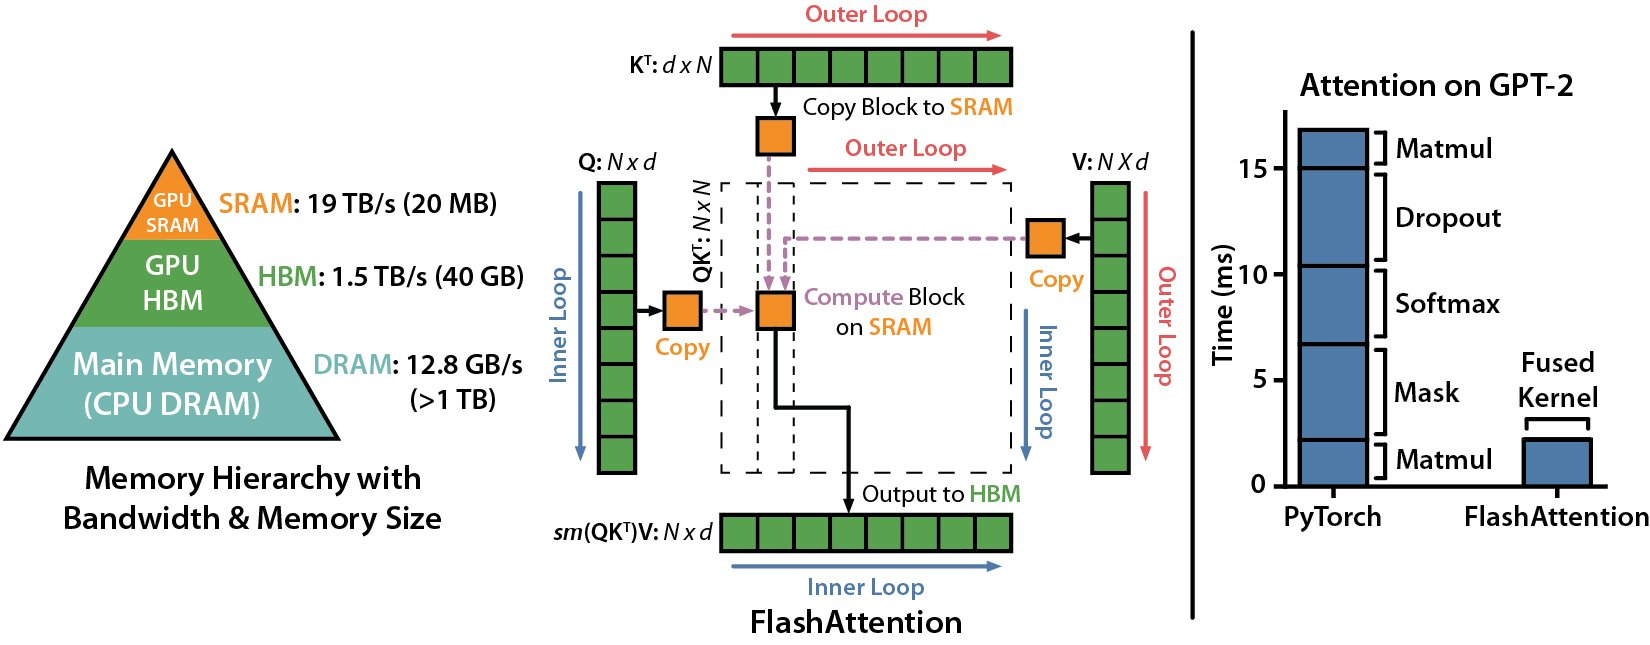
\includegraphics[width=0.85\textwidth]{figures/flashattention_overview.jpg}
\caption{FlashAttention 的存储层次、分块计算与 GPT-2 注意力时间对比。左：GPU 片上 SRAM、HBM 与主机 DRAM 的带宽与容量；中：外循环/内循环分块，把分块拷入 SRAM 计算后写回 HBM；右：PyTorch 实现与融合 kernel 的时间构成。\figsrc{flashattn}}
\label{fig:flashattn}
\end{figure}


\subsection{屋顶线模型与算术强度}

屋顶线（roofline）模型~\cite{roofline} 把一个 kernel 的可达性能表示为
\begin{equation}
  P_{\text{attain}} = \min\bigl(P_{\text{peak}},\; I\cdot BW\bigr),
  \label{eq:roofline}
\end{equation}
其中 $P_{\text{peak}}$ 为峰值算力，$BW$ 为存储带宽，$I$ 为算术强度（每字节访存对应的运算次数）。对一个 $M\times K$ 激活乘 $K\times N$ 权重的 GEMM，若权重不能驻留片上、每次都从片外读取，则
\begin{equation}
  I=\frac{2MNK}{NK\,b_w+(MK+MN)\,b_a}\;\xrightarrow{\;M\ll N,K\;}\;\frac{2M}{b_w}\quad(\text{ops/byte}),
  \label{eq:intensity}
\end{equation}
其中 $b_w$、$b_a$ 分别为权重与激活的字节宽度。式~\eqref{eq:intensity} 的含义是：当行数远小于矩阵维度时，算术强度只由 $M$ 与权重位宽决定。这一关系是理解 VLA 负载与 LLM 解码之间差别的关键，第~\ref{sec:vla} 节会用它定量比较三类 GEMM。

\subsection{FPGA 体系结构要素}

与早期以查找表和通用 DSP 为主的 FPGA 相比，面向 AI 的现代 FPGA 在四个方面发生了显著变化，它们共同决定了 Transformer 类负载在 FPGA 上的映射空间。

\textbf{硬核矩阵单元。} Intel Stratix 10 NX 集成了 3,960 个 AI Tensor Block，每个块含三个点积单元、共 30 个乘法器，基础精度为 INT8/INT4，并以共享指数支持块浮点~\cite{s10nx_fpga21,s10nx_trets}；Xilinx（AMD）Versal ACAP 集成了由最多 400 个 AI Engine 组成的二维 VLIW/SIMD 处理器阵列~\cite{versal_fpga19}；Achronix Speedster7t 集成了机器学习处理器（Machine Learning Processor，MLP）阵列，每个 MLP 块最多含 32 个乘法器，支持 4 至 24 位整数和多种浮点/块浮点模式，厂商资料给出的全器件 INT8 峰值为 40,960 个 MAC、750~MHz 下约 61.4~TOPS~\cite{achronix}。这些硬核之间通常有专用的级联通路，可以在相邻单元之间传递操作数或部分和而不占用通用布线资源。

\textbf{片上存储。} 片上 SRAM 仍以分布式块 RAM 为主，总容量为数十 MB 量级，远小于数十亿参数模型的权重规模。因此，与在 FPGA 上部署卷积网络时常见的“权重全部常驻片上”~\cite{finn,hls4ml} 不同，LLM 与 VLA 的权重必须存放在片外，并按层或按块流入。

\textbf{片外存储。} HBM（如 Alveo U280、VCU128 所用）与 GDDR6（如 Speedster7t 所用）提供数百 GB/s 至 TB/s 量级的带宽。Speedster7t 支持最多 32~GB 外接 GDDR6~\cite{achronix}。

\textbf{片上网络。} Speedster7t 引入了硬化的二维片上网络（Network-on-Chip，NoC），把 GDDR6、PCIe 等接口连接到 fabric 中的 80 多个接入点，厂商资料称其总带宽超过 20~Tbps~\cite{achronix}；Versal 同样提供硬化的 NoC~\cite{versal_fpga19}。NoC 使得“多个独立计算单元各自访问外存”的组织方式成为可能，而不必在 fabric 中布一张大型交叉开关。

对 AI 优化 FPGA 的实测研究表明，硬核峰值并不是决定性因素。Boutros 等~\cite{s10nx_fpt} 在大量实时推理负载上对比 Stratix 10 NX 与 NVIDIA T4/V100 时发现，可达性能主要取决于张量单元利用率与主机数据传输开销；针对 Stratix 10 的“持久化实时 AI”评估工作~\cite{s10_persistent} 则从模型常驻片上、低批量实时推理的角度讨论了器件的增强方向。这些结论在第~\ref{sec:case} 节的案例中会再次得到印证。


\subsection{FPGA 与 GPU 的执行模型差异}\label{sec:execmodel}

理解 FPGA 方案的优势与劣势，需要先对比两类平台的执行模型。GPU 采用单指令多线程（SIMT）的时间复用模型：同一组计算单元按顺序执行一系列 kernel，每个 kernel 在执行期间占用全部或部分流多处理器，数据经多级缓存在片外存储与寄存器之间流动。它的优势在于通用性与成熟的软件栈：新的算子只需编写新的 kernel，编译器与库负责调度；它的代价在于 kernel 启动开销、缓存行为带来的时延不确定性，以及非线性算子与 GEMM 之间的数据往返（除非通过融合消除）。

FPGA 的传统执行模型则是空间数据流：不同算子被实例化为不同的硬件单元，数据在单元之间直接流动，控制在编译或综合时确定。它的优势在于可以为特定模型定制数据通路与数值格式，并消除大部分动态行为；代价在于硬件资源是静态划分的，某一阶段不用的单元在该阶段闲置，而且修改模型往往需要重新综合，周期以小时甚至天计。介于二者之间的是“FPGA 上的可编程处理器阵列”：在 FPGA 上实例化一组固定的计算单元，再由编译器生成程序驱动它们，Brainwave~\cite{brainwave} 的软 NPU、DFX~\cite{dfx} 的自定义指令核以及第~\ref{sec:case} 节案例的节点阵列都属于这一类。它牺牲了部分定制程度，换来了“改模型只需改程序”的灵活性。

对于模型迭代很快的 VLA 领域，这一灵活性相当重要：从 \pizero{} 到 \pihalf{}、从 Octo 到 GR00T N1，模型结构与规模在一两年内就发生了明显变化。一个需要为每个模型重新设计硬件的方案，很难跟上这一节奏；一个以编译器为中心、硬件相对稳定的方案，则可以把模型变化吸收在软件层面。

\subsection{硬核矩阵单元的数据流模式}\label{sec:dataflow}

把 GEMM 映射到硬核阵列时，首先要决定“谁静止、谁流动”。沿用脉动阵列文献的术语，常见的组织有三种。\emph{权重静止}（weight-stationary）把权重分块预先装入各处理单元，激活流过阵列，部分和沿某一方向累加；它适合权重复用度高、即 $M$ 较大的 GEMM。\emph{输出静止}（output-stationary）让每个处理单元负责一个或一组输出元素，激活与权重都流过阵列，累加器在原地积累；它减少了部分和的搬运，但要求两路操作数同时馈送。\emph{输入静止}（input-stationary）让激活驻留，权重流过，适合激活复用度高的场景。

在 FPGA 硬核级联上，这三种组织表现为“级联上传递什么”的选择。若级联传递部分和，则一列硬核共同计算一个点积的不同段，最后一级输出完整结果；这种“部分和级联”与权重静止相容，但每一级只贡献点积的一段，若硬核内部的多路乘法器不能同时参与同一段，便会出现乘法器闲置。若级联传递操作数（广播激活），则每一级独立计算一个输出列的完整点积并在本地累加；这相当于在一列硬核上做“输出静止 + 激活广播”，每一级的全部乘法器都能参与，但每一级需要自己的权重存储与结果引出通路。第~\ref{sec:case} 节的案例采用的正是后一种组织，简报指出它使每级 16 个乘法器在一次行传递中全部忙碌，而部分和级联方案会浪费其中的 15/16。

这一选择的代价在布线上：结果引出通路越多、每级独立的控制越多，占用的通用 fabric 资源越多。FlightLLM~\cite{flightllm} 的“可配置稀疏 DSP 链”与 Stratix 10 NX 的张量块链~\cite{s10nx_fpga21} 分别给出了不同的折中。对于 VLA 这类同时含有大 $M$ 与小 $M$ GEMM 的负载，数据流模式还决定了阵列在两类形状之间切换时的效率损失，第~\ref{sec:shape} 节将对此做定量讨论。

\begin{table}[t]
\centering
\caption{代表性 AI 优化 FPGA 平台的硬核资源（依据所引文献与厂商资料的摘要级信息；“—”表示本文未从可用来源读到）。}
\label{tab:devices}
\small
\begin{tabularx}{\textwidth}{l Y Y Y}
\toprule
器件 & 硬核矩阵单元 & 片上网络 & 外存 \\
\midrule
Intel Stratix 10 NX~\cite{s10nx_fpga21} & 3,960 个 AI Tensor Block；每块 30 个乘法器；INT8/INT4 + Block FP16/FP12 & — & HBM2（据检索报道） \\
AMD Versal ACAP~\cite{versal_fpga19,charm} & 最多 400 个 AI Engine（VLIW/SIMD）；1~GHz 下 fp32 约 6.4~TFLOPs~\cite{charm} & 硬化 NoC & 视型号而定 \\
Achronix Speedster7t~\cite{achronix} & MLP 阵列；每块最多 32 个乘法器；4 至 24 位整数与浮点/块浮点；全器件 40,960 个 INT8 MAC & 硬化二维 NoC，80 余个接入点，总带宽超过 20~Tbps & GDDR6，最多 32~GB \\
AMD Alveo U280（DFX、FlightLLM 等所用） & DSP 硬核 & — & HBM \\
\bottomrule
\end{tabularx}
\end{table}

%======================================================================
\section{VLA 模型：族谱与计算特征}\label{sec:vla}
%======================================================================

\subsection{发展脉络}

VLA 的发展可以大致分为三个阶段。

\textbf{第一阶段：机器人 Transformer。} RT-1~\cite{rt1} 以 FiLM 条件化的 EfficientNet、TokenLearner 与 Transformer 组成策略网络，输入图像与自然语言指令，输出离散化的底盘与机械臂动作。其规模仅 3,500 万参数，能以约 3~Hz 运行，并在大规模真实环境训练与评测中展现了良好的泛化性\hw{真实机器人闭环，约 3~Hz；具体机器人型号本文未从可用来源读到}。同一时期，ACT~\cite{act} 在低成本双臂平台 ALOHA 上\hw{ALOHA 低成本双臂遥操作平台}提出了“动作分块”（action chunking）：策略一次预测未来一段动作序列而不是单步动作，从而减轻复合误差并提升时间一致性。Diffusion Policy~\cite{diffpolicy} 则把视觉运动策略表示为动作空间中的条件去噪扩散过程，能够自然地表达多峰动作分布，并引入滚动时域执行。这三项工作分别奠定了后续 VLA 的三个基本要素：Transformer 骨干、动作分块与生成式动作头。

\textbf{第二阶段：以 VLM 为骨干的 VLA。} RT-2~\cite{rt2} 首次把大规模预训练 VLM 直接用作机器人策略，把动作离散化为文本 token，与互联网规模的视觉-语言数据共同微调，使机器人获得了对未见物体与语义指令的泛化能力。据检索到的论文正文，其 550 亿参数版本无法直接在机器人端常用的 GPU 上运行，而是部署在多 TPU 的云端服务上、由机器人经网络查询，控制频率约 1 至 3~Hz；50 亿参数版本约 5~Hz\hw{多 TPU 云端推理服务，经网络查询}。Open X-Embodiment~\cite{oxe} 提供了标准化格式的跨形态数据集与 RT-X 模型，覆盖 22 种机器人形态、逾百万条真实轨迹（图~\ref{fig:oxe}），为后续开放模型的训练奠定了数据基础\hw{22 种机器人形态，从单臂、双臂到四足}。Octo~\cite{octo} 是基于 Transformer 的开放通用策略，用扩散解码输出动作，在约 80 万条轨迹上预训练，有 2,700 万与 9,300 万参数两个规模（图~\ref{fig:octo}）。据其论文，预训练在 TPU 上完成，在单块 24~GB 显存的 GPU 上微调约需 5 小时，实验机器人包括 WidowX、UR5 与 Franka 等\hw{训练：TPU；微调：单块 24~GB GPU；机器人：WidowX、UR5、Franka 等 9 种平台}。OpenVLA~\cite{openvla} 是一个 70 亿参数的开放 VLA，以 Llama 2 为语言骨干、融合 DINOv2 与 SigLIP 视觉特征，在约 97 万条真实示教上训练，沿用了 RT-2 的离散动作 token 路线。官方代码库给出的 LoRA 微调配置为单块 80~GB 显存的 A100；在 A100 上其动作生成吞吐约 4.2~Hz、时延约 0.240~s（图~\ref{fig:oftefficiency}）\hw{微调：A100 80~GB；推理：A100}。
\begin{figure}[t]
\centering
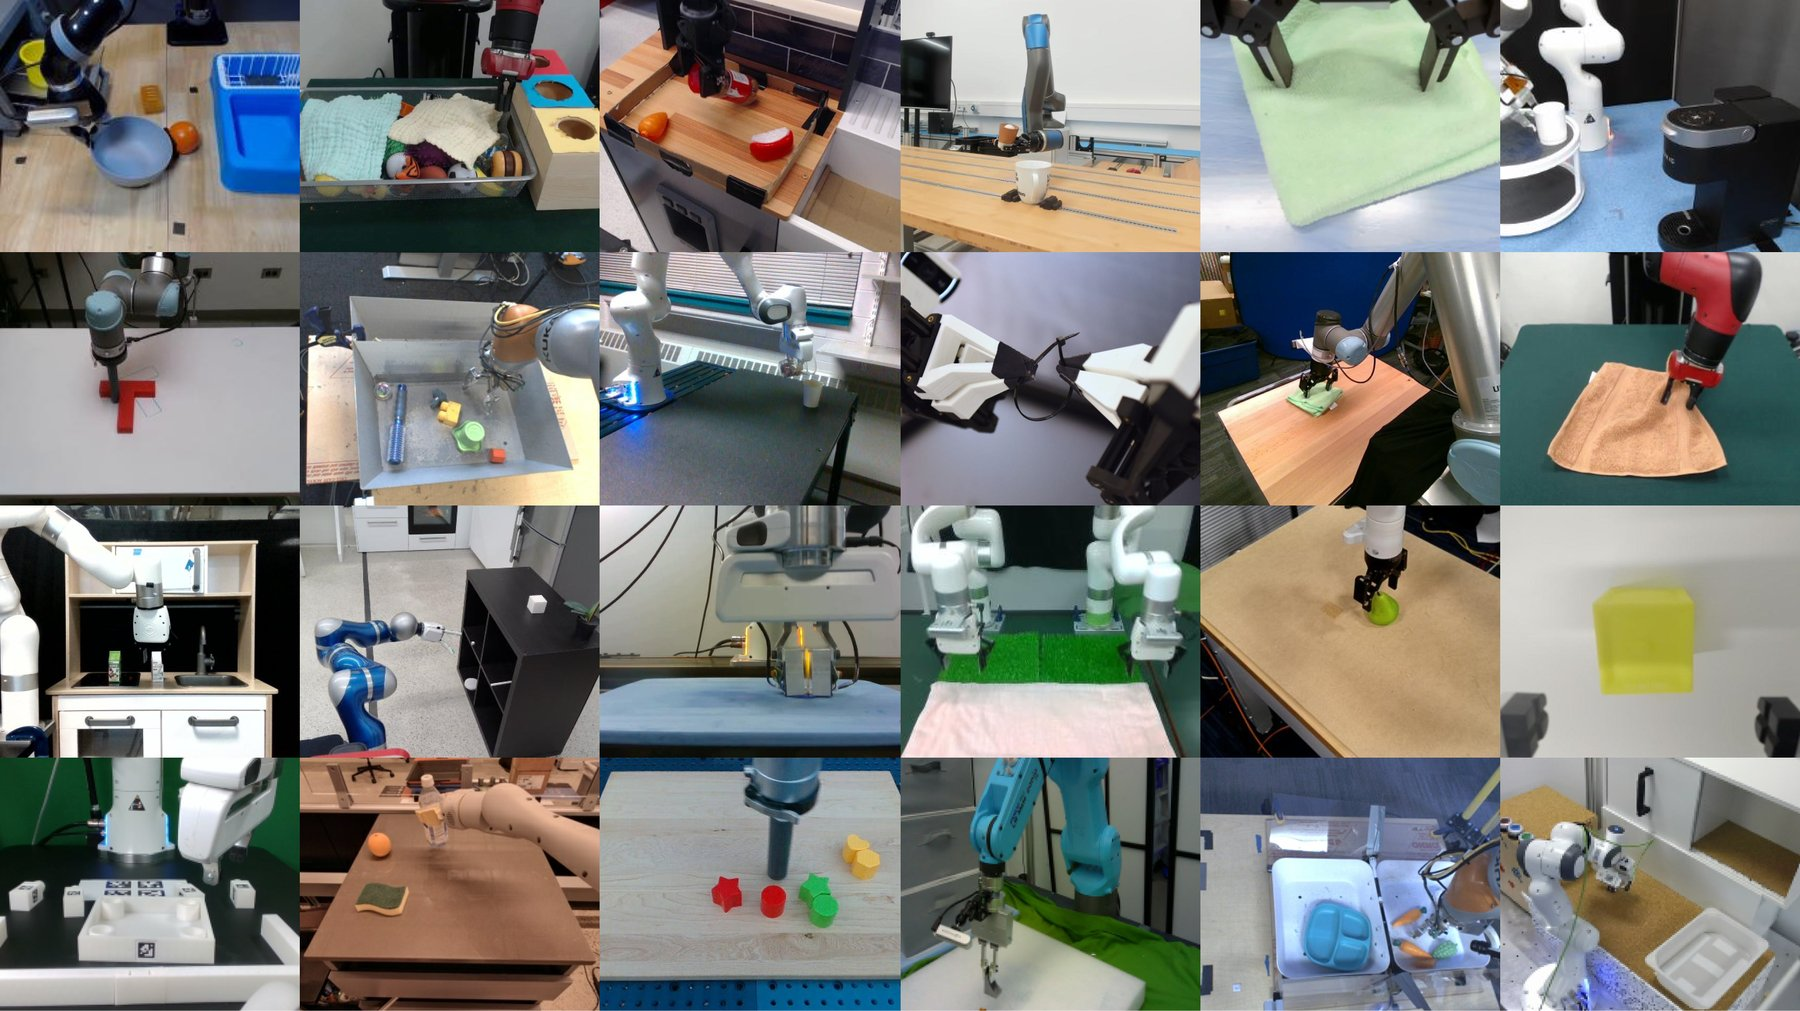
\includegraphics[width=0.78\textwidth]{figures/oxe_teaser.jpg}
\caption{Open X-Embodiment 数据集涵盖的部分机器人与场景。\figsrc{oxe}}
\label{fig:oxe}
\end{figure}

\begin{figure}[t]
\centering
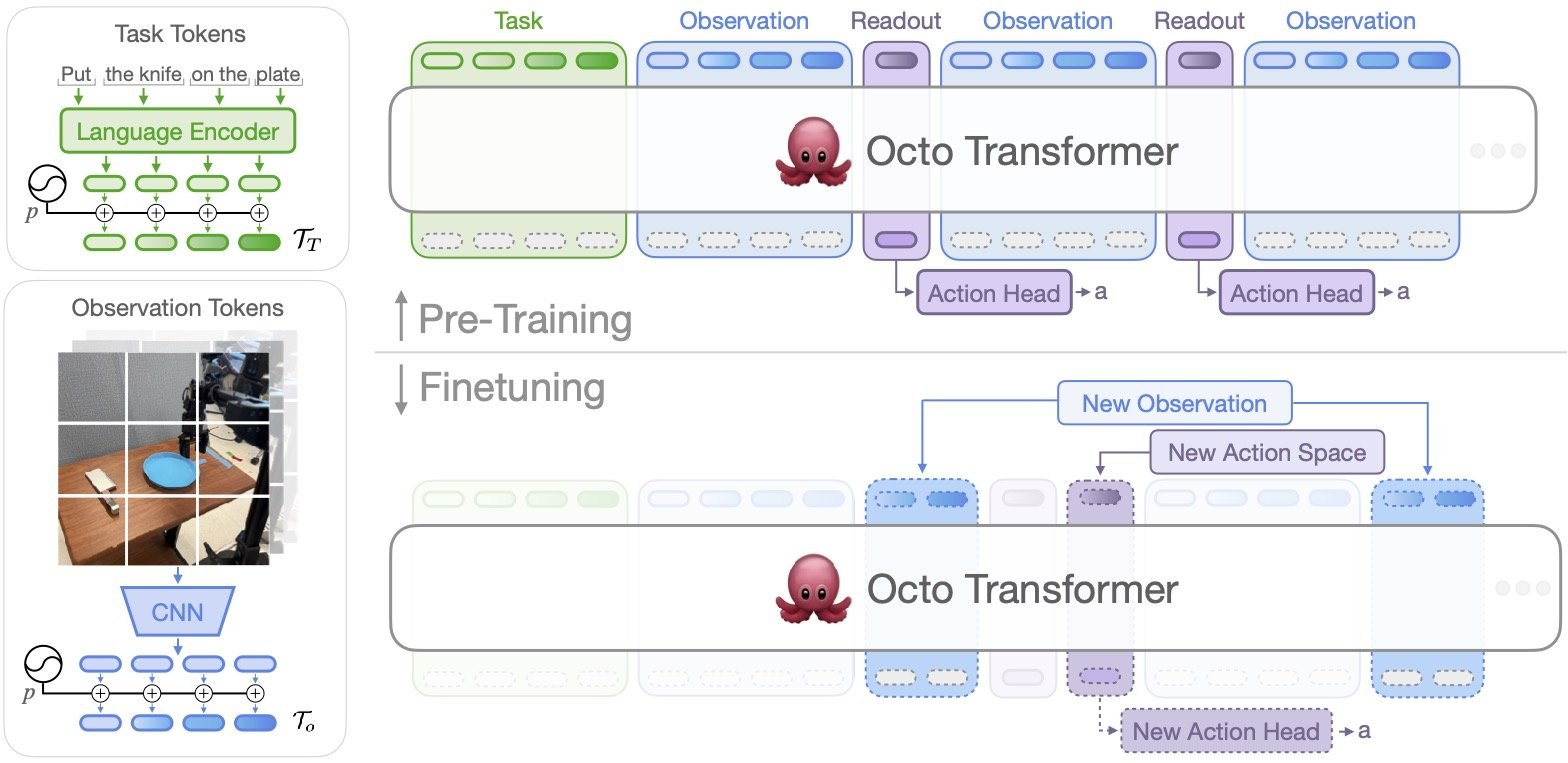
\includegraphics[width=0.85\textwidth]{figures/octo_arch.jpg}
\caption{Octo 的模型结构。任务 token（语言编码器）与观测 token（CNN 图像分块）输入 Octo Transformer，经读出（readout）token 连接动作头；微调时可添加新的观测输入与新的动作头。\figsrc{octo}}
\label{fig:octo}
\end{figure}


\textbf{第三阶段：VLM 骨干 + 连续动作生成。} \pizero~\cite{pi0} 在 PaliGemma~\cite{paligemma} VLM 上增加一个参数独立的“动作专家”，以流匹配~\cite{flowmatching} 方式生成连续动作块，在多种机器人平台的复杂灵巧任务上取得了当时领先的结果。其官方代码库 openpi 给出的推理需求为显存 8~GB 以上（示例 GPU 为 RTX 4090），全参数微调需要 A100（80~GB）或 H100，并提供针对 ALOHA 与 DROID 平台的微调检查点\hw{推理：RTX 4090 级 GPU；微调：A100 80~GB / H100；机器人：自有平台、ALOHA、DROID}。\pihalf~\cite{pi05} 在 \pizero{} 基础上引入多来源异构数据的协同训练与高层语义子任务预测，能在未见过的家庭环境中执行 10 至 15 分钟的长程任务\hw{移动操作机器人}。FAST~\cite{fast} 用基于离散余弦变换的压缩分词重新激活了自回归路线，使其能处理高频灵巧任务。GR00T N1~\cite{gr00t} 采用“双系统”结构：VLM 模块（System 2）负责理解，扩散 Transformer 模块（System 1）负责生成动作，二者端到端联合训练（图~\ref{fig:gr00t}）。其摘要报告部署于 Fourier GR-1 人形机器人；官方代码库当前版本（N1.7）列出的推理平台包括 RTX 4090、L40、H100、Jetson AGX Thor/Orin 与 DGX Spark\hw{机器人：Fourier GR-1；推理：16~GB 以上显存 GPU，含 Jetson AGX Thor/Orin}。RDT-1B~\cite{rdt} 把基于扩散的机器人基础模型扩展到 12 亿参数，并提出物理可解释的统一动作空间（图~\ref{fig:rdt}）；其官方代码库说明模型部署于 ALOHA 双臂机器人\hw{ALOHA 双臂机器人}。SmolVLA~\cite{smolvla} 则反向而行，把整套方案压缩到约 4.5 亿参数，面向消费级 GPU 乃至 CPU 部署，并在低成本的 SO-100 机械臂上评测\hw{消费级 GPU / CPU；机器人：SO-100}。
\begin{figure}[t]
\centering
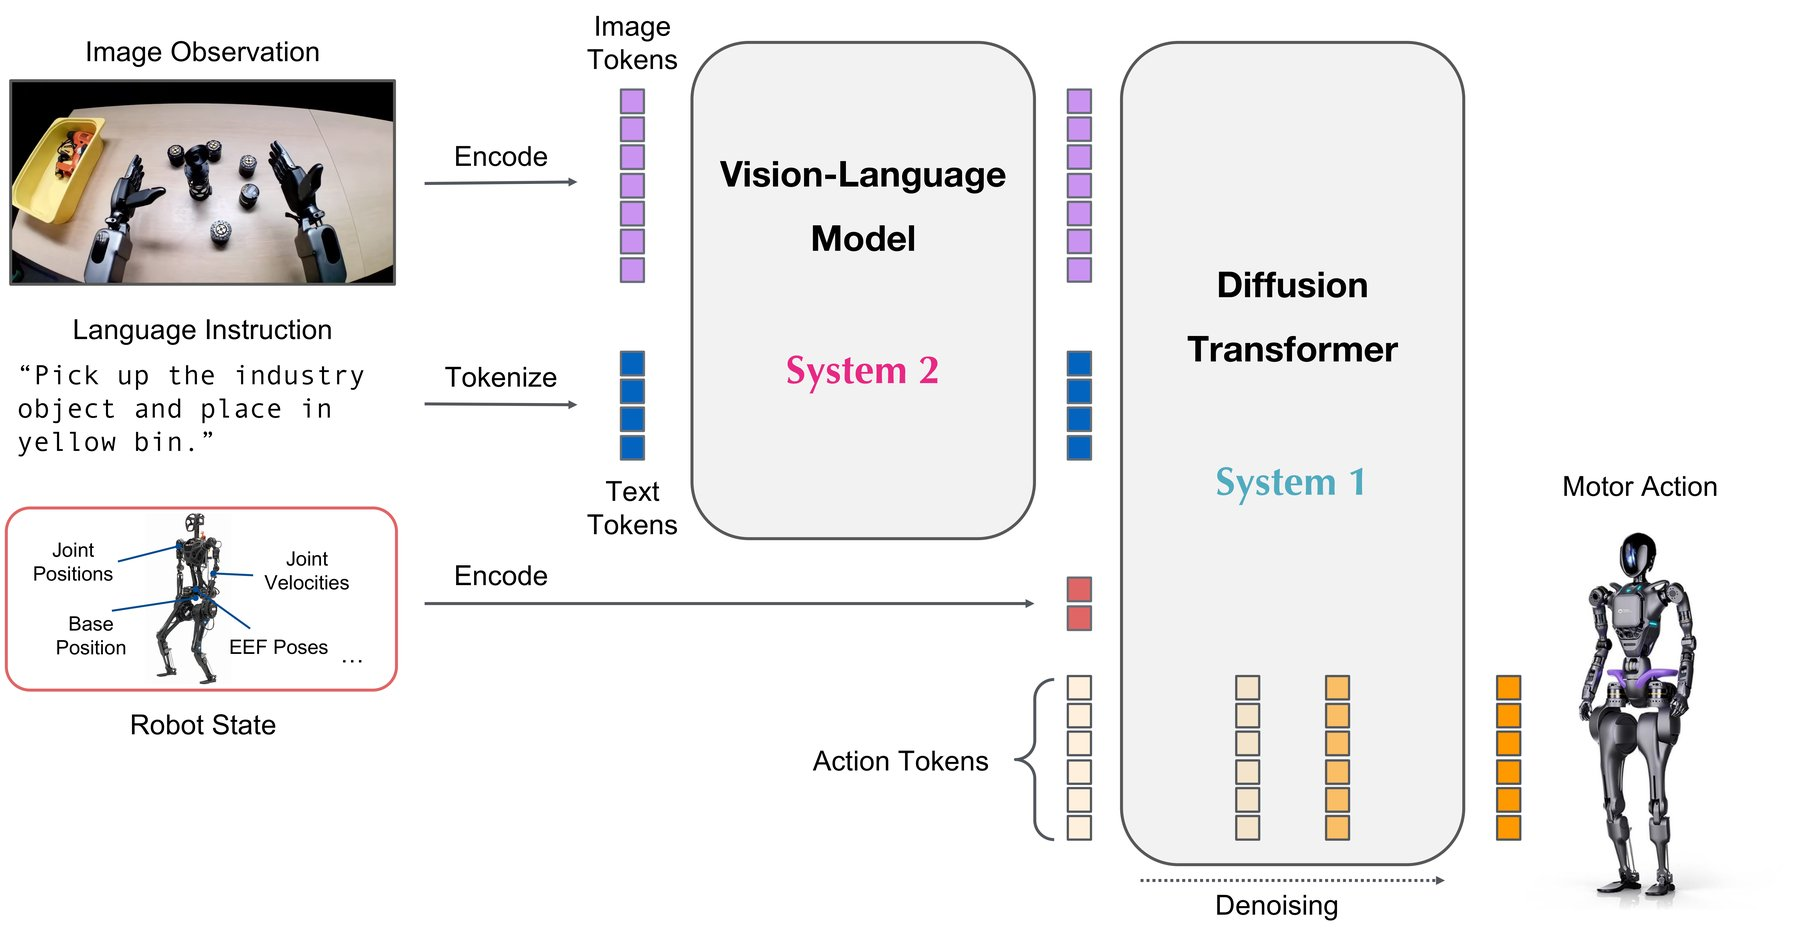
\includegraphics[width=0.85\textwidth]{figures/gr00t_n1_arch.jpg}
\caption{GR00T N1 的双系统结构：视觉-语言模型（System 2）编码图像与语言 token，扩散 Transformer（System 1）结合机器人状态对动作 token 去噪，输出电机动作。\figsrc{gr00t}}
\label{fig:gr00t}
\end{figure}

\begin{figure}[t]
\centering
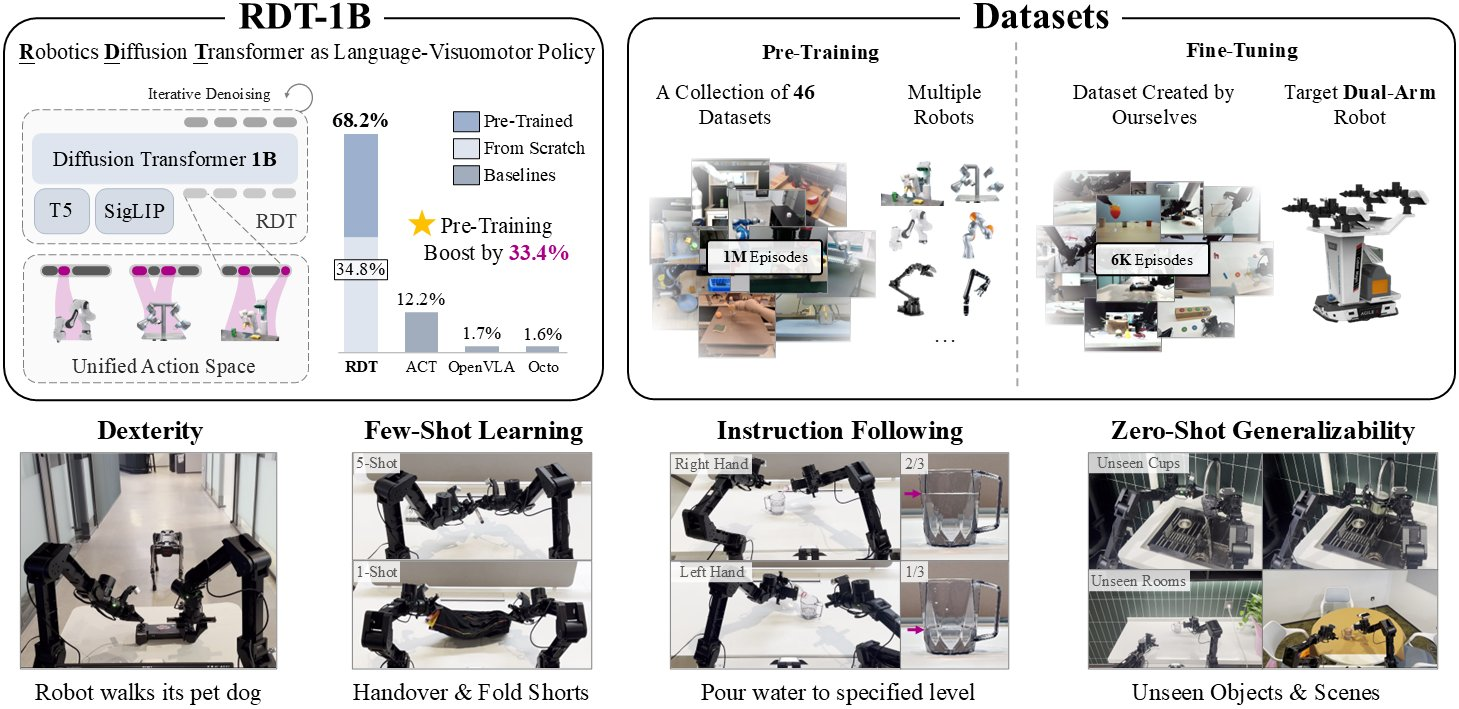
\includegraphics[width=0.85\textwidth]{figures/rdt1b_overview.jpg}
\caption{RDT-1B 概览：以 SigLIP 与 T5 编码输入、1B 参数扩散 Transformer 迭代去噪并使用统一动作空间；在 46 个数据集约 100 万回合上预训练，在约 6K 回合自采双臂数据上微调。\figsrc{rdt}}
\label{fig:rdt}
\end{figure}


\subsection{按动作表示的分类法}

从部署视角，决定 VLA 推理形态的首要因素是动作的表示与生成方式，其次才是骨干网络规模。本文据此把 VLA 分为三类（表~\ref{tab:vla}）。

\textbf{（1）离散 token 自回归。} 动作被离散化为 token，与文字一样逐个解码，代表工作为 RT-2~\cite{rt2}、OpenVLA~\cite{openvla} 与 \pizero-FAST~\cite{fast}。其推理形态与 LLM 完全相同：一次前缀预填充，接若干步 $M=1$ 的解码。它可以直接继承 LLM 推理栈的全部优化，但也继承了 LLM 解码的带宽瓶颈；每个动作块的解码步数等于动作 token 数，FAST 的意义正在于通过压缩减少这一数目。OpenVLA-OFT~\cite{openvlaoft} 则走得更远，改用并行解码、动作分块、连续动作表示与 L1 回归目标，据其摘要把动作生成吞吐提升约 26 倍。这一结果说明，逐 token 自回归并不是动作生成的必需形态。

\textbf{（2）扩散动作头。} 动作由一个条件去噪网络经多步迭代生成，代表工作为 Diffusion Policy~\cite{diffpolicy}、Octo~\cite{octo}、GR00T N1~\cite{gr00t} 与 RDT-1B~\cite{rdt}，去噪网络常采用扩散 Transformer（DiT）~\cite{dit} 结构。推理形态为“一次条件编码 + $S$ 次去噪网络前向”，每次前向处理整个动作块（图~\ref{fig:diffpolicy}）。以 Diffusion Policy 为例，据检索到的论文正文，其真实机器人实验采用 DDIM，以 10 步推理在 NVIDIA RTX 3080 上达到约 0.1~s 的时延\hw{NVIDIA RTX 3080}。
\begin{figure}[t]
\centering
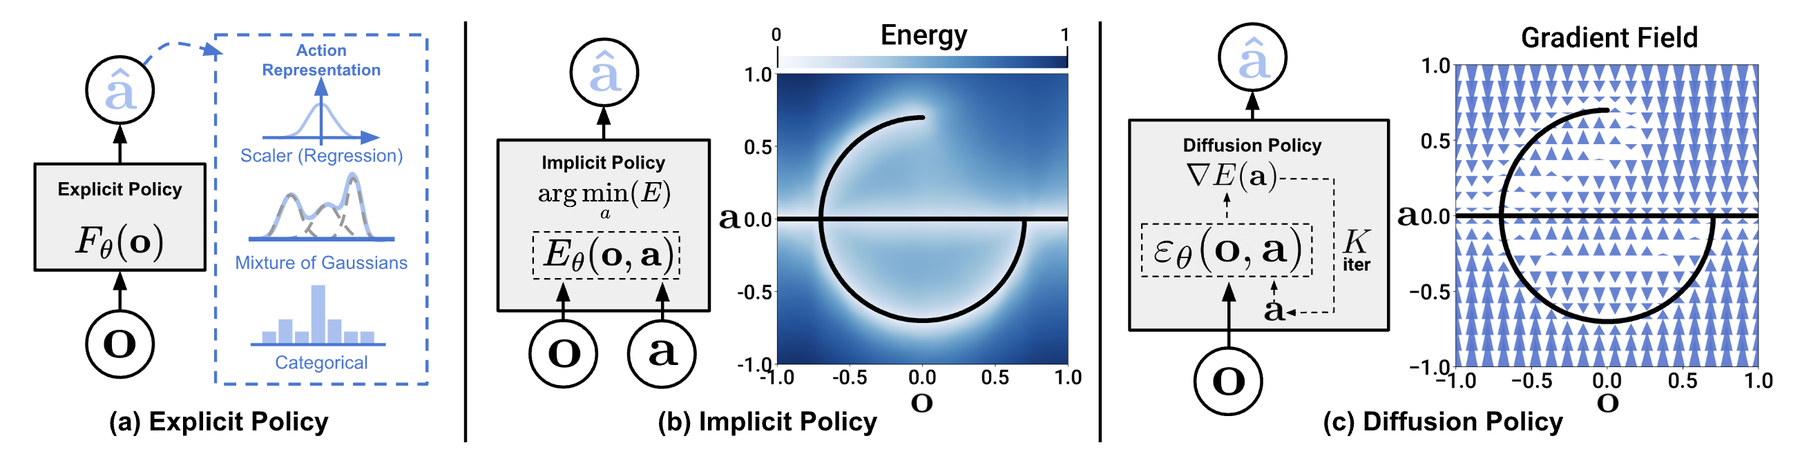
\includegraphics[width=0.95\textwidth]{figures/diffusion_policy_teaser.png}
\caption{三类策略表示的对比：(a) 显式策略直接回归动作；(b) 隐式策略以能量函数的 argmin 求动作；(c) 扩散策略以噪声预测网络迭代 $K$ 次，沿梯度场生成动作。\figsrc{diffpolicy}}
\label{fig:diffpolicy}
\end{figure}


\textbf{（3）流匹配动作专家。} 流匹配~\cite{flowmatching} 通过回归固定条件概率路径上的向量场训练连续归一化流，与扩散相比训练更稳定，推理时可用少量常微分方程积分步完成。代表工作为 \pizero~\cite{pi0}、\pihalf~\cite{pi05} 与 SmolVLA~\cite{smolvla}。从硬件角度看，流匹配与扩散的推理形态同构：都是对同一个网络做 $S$ 次迭代前向，差别主要在步数与更新公式。

在结构上，第（2）、（3）类又常采用“VLM 骨干 + 独立动作网络”的组织：动作网络通过交叉注意力或共享注意力读取 VLM 的中间表示或 KV cache。这种组织把一次推理拆成两段形状迥异的负载，是 VLA 部署问题的核心特征。

\begin{table}[t]
\centering
\caption{代表性 VLA 模型的部署相关特征。数字来自对应文献的摘要级信息或项目简报；“—”表示本文未从可用来源读到。}
\label{tab:vla}
\small
\begin{tabularx}{\textwidth}{l Y l Y}
\toprule
模型 & 骨干 / 规模 & 动作生成方式 & 部署相关特征 \\
\midrule
RT-1~\cite{rt1} & EfficientNet + Transformer，3,500 万 & 离散动作 & 约 3~Hz；模型小 \\
RT-2~\cite{rt2} & 大型 VLM & 离散 token 自回归 & 形态同 LLM，解码带宽受限 \\
OpenVLA~\cite{openvla} & Llama 2 + DINOv2/SigLIP，70 亿 & 离散 token 自回归 & OFT~\cite{openvlaoft} 改为并行解码输出整块 \\
\pizero-FAST~\cite{fast} & PaliGemma 系 & DCT 压缩 token 自回归 & 解码步数随压缩率下降 \\
Octo~\cite{octo} & Transformer，2,700 万 / 9,300 万 & 扩散头 & 模型小，端侧易部署 \\
GR00T N1~\cite{gr00t} & VLM + DiT，20 亿检查点 & 扩散 Transformer & 双系统，可异步 \\
RDT-1B~\cite{rdt} & 扩散 Transformer，12 亿 & 扩散 & 统一动作空间 \\
\pizero~\cite{pi0} & PaliGemma + 约 3 亿参数动作专家 & 流匹配 & 本文案例：10 步 Euler，前缀 $M\approx525$，专家 $M=51$ \\
\pihalf~\cite{pi05} & 基于 \pizero & 流匹配 + 语义预测 & 长程任务，层级推理 \\
SmolVLA~\cite{smolvla} & 约 4.5 亿 & 流匹配 & 面向消费级硬件 \\
\bottomrule
\end{tabularx}
\end{table}

\subsection{计算特征剖析：以 \texorpdfstring{\pizero{}}{pi0} 为例}\label{sec:pi0profile}

本节以第~\ref{sec:case} 节案例所部署的 \pizero{} 为例，定量刻画流匹配 VLA 的推理负载。按项目简报，其结构如下：视觉编码器为 SigLIP~\cite{siglip} So400m/14（27 层，宽 1152，16 头 $\times$ 72）；语言模型为 Gemma-2B~\cite{gemma}（18 层，宽 2048，MLP 宽 16384，采用 GeGLU，8 个查询头 $\times$ 256，共享 1 个 KV 头）；动作专家约 3 亿参数（Gemma 结构，18 层，宽 1024，MLP 4096），关注 VLM 的 KV cache。动作由流匹配生成：每次推理做 10 个 Euler 积分步，输出 50 个未来动作组成的动作块。检查点在 DROID~\cite{droid} 数据集上微调，该数据集用 Franka Panda 7 自由度机械臂采集，约 7.6 万条轨迹、350 小时交互数据，其硬件配置见图~\ref{fig:droid}\hw{Franka Panda 7 自由度机械臂、Robotiq 2F-85 夹爪、2 台 Zed 2 立体相机与 1 台腕部 Zed Mini 相机}。
\begin{figure}[t]
\centering
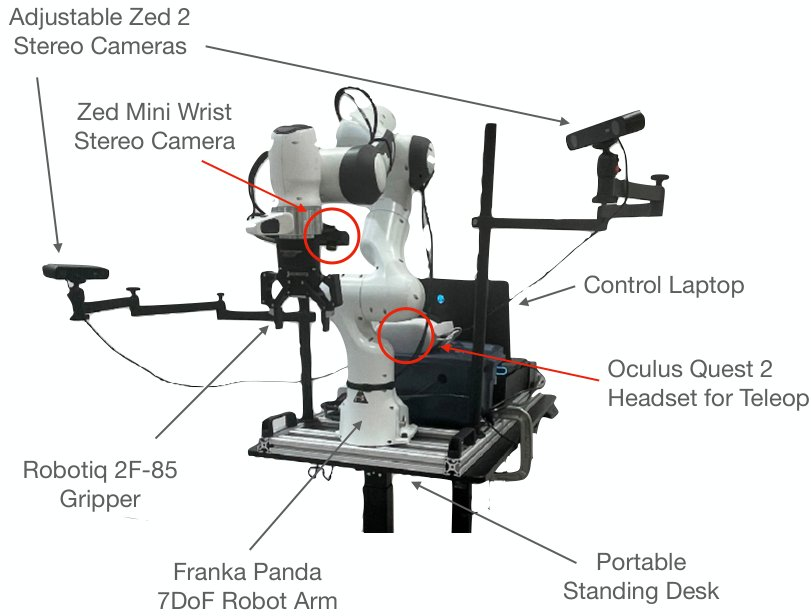
\includegraphics[width=0.55\textwidth]{figures/droid_setup.jpg}
\caption{DROID 的数据采集平台：Franka Panda 7 自由度机械臂、Robotiq 2F-85 夹爪、两台可调 Zed 2 立体相机、腕部 Zed Mini 立体相机、用于遥操作的 Oculus Quest 2 头显与控制笔记本。\figsrc{droid}}
\label{fig:droid}
\end{figure}


\begin{figure}[t]
\centering
\begin{tikzpicture}[font=\small, >=Stealth,
  blk/.style={draw, rounded corners=2pt, align=center, minimum height=9mm, inner sep=3pt, fill=#1},
  blk/.default=white]
\node[blk=gray!10, text width=1.7cm] (img) {2 路相机\\图像};
\node[blk=blue!8, text width=2.2cm, right=6mm of img] (sig) {SigLIP\\27 层\\$2\times256$ token};
\node[blk=gray!10, text width=1.6cm, below=5mm of img] (txt) {语言指令\\token};
\node[blk=blue!15, text width=2.6cm, right=8mm of sig] (gem) {Gemma-2B 前缀\\18 层，525 token\\$M\approx525$};
\node[blk=yellow!15, text width=1.9cm, right=8mm of gem] (kv) {前缀 KV cache\\18 层 $\times$ 1 头};
\node[blk=orange!15, text width=3.0cm, below=12mm of kv] (exp) {动作专家（18 层）\\51 token（状态 + 50 动作）\\$M=51$};
\node[blk=gray!10, text width=2.0cm, left=10mm of exp] (out) {动作块\\50 步 $\times$ 7 维};
\draw[->] (img) -- (sig); \draw[->] (sig) -- (gem); \draw[->] (txt) -| (gem);
\draw[->] (gem) -- (kv); \draw[->] (kv) -- node[right, align=left, font=\footnotesize]{每步每层\\重读} (exp);
\draw[->] (exp.east) -- ++(6mm,0) |- ++(0,9mm) node[pos=0.75, above, font=\footnotesize]{Euler 更新，共 10 步} -| ([xshift=4mm]exp.north);
\draw[->] (exp) -- (out);
\end{tikzpicture}
\caption{\pizero{} 一次推理（一个 chunk）的数据流。前缀只计算一次，动作专家迭代 10 步，每步在每一层读取前缀 KV。}
\label{fig:pi0flow}
\end{figure}

\textbf{一个 chunk 的计算构成。} 图~\ref{fig:pi0flow} 给出一次推理（下称“一个 chunk”）的数据流：两路相机图像经 SigLIP 编码为 $2\times256$ 个视觉 token；视觉 token 与语言 token 组成 525 个 token 的前缀，经 Gemma-2B 做一次前缀计算，生成 KV cache；动作专家对 51 个 token（1 个状态 + 50 个动作）迭代 10 步，每步关注 525 个前缀键与自身的键。简报给出每个 chunk 约 1.47~TMAC \tP。为便于读者核对这一量级，本文按上述结构参数做一个粗略自检 \tE：

\begin{itemize}
  \item Gemma-2B 前缀：每层线性层权重约 $2048^2\times2 + 2048\times256\times2 + 3\times2048\times16384 \approx 1.10\times10^8$，18 层合计约 $1.98\times10^9$，乘以 525 个 token 约 1.04~TMAC；
  \item SigLIP：每层约 $4\times1152^2+2\times1152\times4304\approx1.5\times10^7$（MLP 宽度 4304 为 So400m 的公开配置，本文未从简报读到，属估算输入），27 层、512 个 token 约 0.21~TMAC；
  \item 动作专家：每层约 $1024\times2048\times2+1024\times256\times2+3\times1024\times4096\approx1.73\times10^7$，18 层、51 个 token、10 步约 0.16~TMAC；
  \item 注意力矩阵乘：为数十 GMAC 量级。
\end{itemize}
合计约 1.4 至 1.5~TMAC，与简报的 1.47~TMAC \tP{} 一致。自检的意义在于比例：前缀计算（SigLIP 与 Gemma-2B）约占 85\% 的 MAC，动作专家约占 11\%，其余为注意力。

\textbf{三类 GEMM 的算术强度。} 代入式~\eqref{eq:intensity}，INT8 权重（$b_w=1$）下：
\begin{itemize}
  \item 前缀 GEMM（$M\approx525$）：强度上限约 1,050~ops/byte。只要片上缓冲能容纳足够大的权重分块，它是算力受限的；简报对此的表述是“激活的反复重流占主导”（activation re-streaming dominates），即瓶颈转为片上缓冲容量与激活重读。
  \item 动作专家 GEMM（$M=51$）：强度只有约 102~ops/byte，且每个积分步都要把全部专家权重再走一遍。简报称之为“权重搬运受限”（weight-movement-bound）。
  \item LLM 自回归解码（$M=1$）：强度约 2~ops/byte，是 FlightLLM~\cite{flightllm}、DFX~\cite{dfx}、EdgeLLM~\cite{edgellm} 等工作的主要对象。
\end{itemize}
VLA 的动作头因此处在预填充与解码之间的“中间地带”：它对带宽敏感，却不能像解码那样用“带宽 $\times$ 位宽”一个量刻画。图~\ref{fig:roofline} 以示意方式把三类 GEMM 放在屋顶线上。VLA-Perf~\cite{vlaperf} 以解析模型独立给出了类似的结论：\pizero{} 去噪动作阶段的运算强度随动作块长度近似线性增长，动作块长度为 50 时约为 100~FLOPs/Byte，仍低于 B100 的“平衡运算强度”218.8~FLOPs/Byte（图~\ref{fig:vlaperfoi}）\hw{NVIDIA B100（解析模型）}。这与本文按式~\eqref{eq:intensity} 对 $M=51$ 的估算（约 102~ops/byte）处于同一量级；二者的数值精度假设可能不同，只宜比较量级。
\begin{figure}[t]
\centering
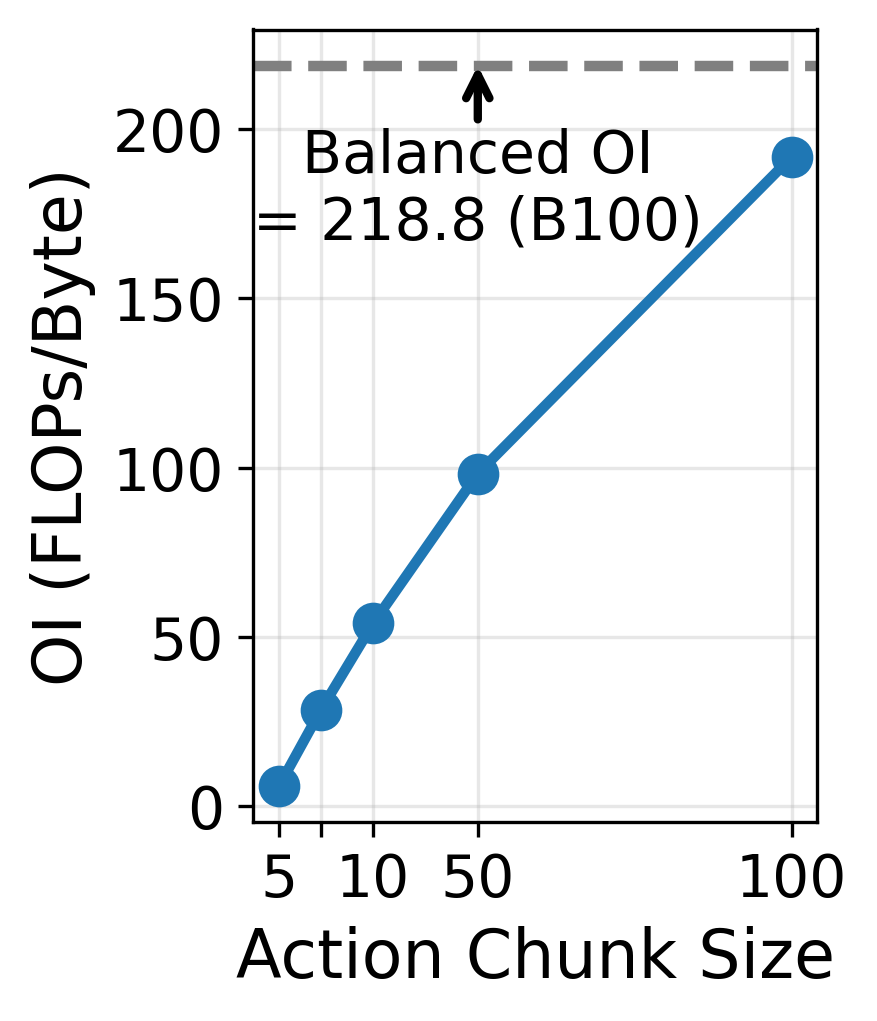
\includegraphics[width=0.36\textwidth]{figures/vlaperf_pi0_oi.png}
\caption{VLA-Perf 给出的 \pizero{} 去噪动作阶段运算强度与动作块长度的关系（B100 解析模型），虚线为 B100 的平衡运算强度。\figsrc{vlaperf}}
\label{fig:vlaperfoi}
\end{figure}


\begin{figure}[t]
\centering
\begin{tikzpicture}
\begin{axis}[
  width=0.72\textwidth, height=5.6cm,
  xmode=log, ymode=log,
  xmin=1, xmax=5000, ymin=0.5, ymax=2000,
  xlabel={算术强度 $I$（ops/byte，对数坐标）},
  ylabel={可达性能（归一化）},
  ytick=\empty, yticklabels={},
  grid=major, grid style={gray!20},
  font=\small]
\addplot[thick, black, domain=1:5000, samples=200] {min(x, 400)};
\addplot[only marks, mark=*, mark size=2.5pt, red] coordinates {(2,2)};
\addplot[only marks, mark=square*, mark size=2.5pt, orange] coordinates {(102,102)};
\addplot[only marks, mark=triangle*, mark size=3pt, blue] coordinates {(1050,400)};
\node[anchor=west, font=\footnotesize] at (axis cs:2.3,2) {LLM 解码 $M=1$};
\node[anchor=west, font=\footnotesize] at (axis cs:115,85) {动作专家 $M=51$};
\node[anchor=north, font=\footnotesize] at (axis cs:1050,330) {前缀 $M\approx525$};
\node[anchor=south, font=\footnotesize] at (axis cs:2500,420) {$P_{\text{peak}}$};
\end{axis}
\end{tikzpicture}
\caption{三类 GEMM 在屋顶线模型上的位置（示意图，INT8 权重、权重从片外读取；屋顶拐点位置取决于具体器件，此处仅为示意）。}
\label{fig:roofline}
\end{figure}

\textbf{权重流量。} INT8 下每个 chunk 的最小片外权重流量 \tE：VLM 前缀（SigLIP 与 Gemma-2B）线性层权重约 2.4~GB，每个 chunk 至少读一遍；动作专家权重约 0.31~GB，若不能驻留片上，10 步共读约 3.1~GB。也就是说，\emph{动作专家的计算量只占约 11\%，其权重流量却超过总权重流量的一半}。这是流匹配 VLA 与纯 LLM 推理最显著的访存差异，也是后文讨论“专家权重驻留”与“步间权重复用”的出发点。

\textbf{KV cache。} Gemma-2B 只有 1 个 KV 头（头宽 256），前缀 KV 的规模为 $525\times18\times2\times256$ 个元素，bf16 下约 9.7~MB，INT8 下约 4.8~MB \tE。动作专家每个积分步都要在每一层重读这份 KV，10 步即重读 10 遍。对 FPGA 而言，这个量级处在“可能驻留片上”的范围：按简报，器件有 2,560 块 BRAM72K，若按名义容量每块 72~Kb 计算，合计约 23~MB \tD（$2560\times72~\text{Kb}\div8$），与 KV 大小同一量级。这是 LLM 长上下文解码中不存在的机会：VLA 的前缀短而固定，KV 被高频复用。

\textbf{非线性算子。} 如第~\ref{sec:bg} 节所述，归一化、softmax、激活、RoPE、残差与量化相关运算几乎不贡献 MAC，却处在 GEMM 之间的关键路径上。在 GPU 上，它们通过 kernel 融合与 FlashAttention~\cite{flashattn} 一类的分块技术被隐藏在 GEMM 的访存阴影中；在自研加速器上，如果向量通路的吞吐没有随矩阵阵列同比例扩展，它们会按 Amdahl 定律成为主导项。第~\ref{sec:case} 节的案例正是这一现象的直接证据。

\textbf{迭代依赖。} 流匹配的 10 个积分步之间有严格的数据依赖：第 $k+1$ 步的输入是第 $k$ 步 Euler 更新后的动作。因此在单个 chunk 内，各步只能流水而不能并行；能够复用的是各步共享的前缀 KV 与完全相同的专家权重，能够并行的是步内 51 个 token 之间的行并行。这与扩散模型的多步去噪同构，但与 LLM 解码“每步只多一个 token”不同：流匹配每步都要重算全部 51 个 token 的完整前向。

\subsection{数值精度与误差传播}\label{sec:precision}

VLA 的数值精度问题与 LLM 有三点不同，它们共同决定了量化方案在 VLA 上的可用空间。

\textbf{误差沿迭代积累。} 流匹配与扩散动作头对同一网络做 $S$ 次迭代前向，每一步的输出都是下一步的输入。若每步引入的量化误差相互独立且量级相近，最终误差大致随步数累积；若误差存在系统性偏差（例如某一层的截断总是偏向同一方向），累积会更快。LLM 解码中每步只输出一个 token，其误差通过采样被“离散化”，对后续步骤的影响方式不同。

\textbf{误差沿动作块传播。} 一个动作块包含数十个时间步的连续动作，机械臂按顺序执行。动作块内部的误差会表现为轨迹的偏移或抖动，而关节空间的小误差经运动学放大后，可能在末端执行器上表现为可观的位置误差。因此，以关节角误差衡量的开环精度，需要结合具体机器人的运动学与任务的精度要求来解读。

\textbf{误差经闭环放大或纠正。} 在闭环中，策略会根据新的观测修正动作，部分误差能被纠正；但若误差导致机器人进入训练分布之外的状态，策略的后续输出可能进一步恶化。这正是开环指标与闭环成功率之间关系不简单的原因~\cite{vlaquantbench}。

从硬件角度看，这三点意味着：（1）逐层敏感度分析比整模型统一位宽更重要，不同层对最终动作误差的贡献可能相差悬殊；（2）累加精度与非线性算子的精度同样重要，块浮点~\cite{msfp,mx} 以较宽的累加器配合窄位宽操作数，是一种有吸引力的折中；（3）验证流程必须包含以动作为准的指标，而不能只看张量级的信噪比。

\subsection{机器人闭环对推理系统的要求}\label{sec:loop}

机器人策略运行在感知—推理—执行的闭环中。与离线或在线的 LLM 服务相比，它对推理系统至少提出三点不同的要求。

\textbf{时延直接进入控制回路。} 在动作分块执行下，策略一次输出未来 $H$ 步动作（案例中 $H=50$），执行器按控制频率 $f_{\text{ctrl}}$ 逐步执行。若推理时延小于一个动作块的执行时长，就可以在执行当前块的同时计算下一块，实现不停顿的连续控制。设执行视野为 $H_{\text{exec}}\le H$，异步执行要求
\begin{equation}
  T_{\text{inf}} + T_{\text{io}} \le \frac{H_{\text{exec}}}{f_{\text{ctrl}}},
  \label{eq:async}
\end{equation}
同时反应滞后约为 $T_{\text{inf}}+T_{\text{io}}$，其中 $T_{\text{io}}$ 包含相机采集、传输与主机调度。Real-Time Chunking（RTC）~\cite{rtc} 系统讨论了这一问题：同步执行会在块边界产生停顿，朴素的异步执行又会在块边界产生分布外的跳变；RTC 在执行当前块时生成下一块，“冻结”必然被执行的动作并对其余部分做补全（inpainting），据其报告对推理延迟有较强的鲁棒性。这意味着，在异步执行下，推理时延决定的是反应滞后与块间一致性，而不是“能不能跑”；可接受的时延上界与任务的动态性强相关。案例项目的简报给出主机开销约 47~ms/次调用，这个数字本身已占 Thor 端整个 chunk 时延（125.3~ms \tM）的约 38\% \tD（$47/125.3$）。在百毫秒以内的目标区间，系统级开销与加速器内核同等重要。

\textbf{抖动比平均时延更要紧。} 控制器按固定周期调度，一次偶发的长尾时延就可能导致动作队列耗尽、机械臂停顿，或迫使 RTC 类算法冻结更长的前缀。GPU 与 SoC 上的推理受动态调频、内存控制器仲裁、操作系统调度与共享缓存干扰的影响，尾时延难以从结构上保证。确定性执行的加速器更容易给出最坏情况时延的上界：Groq TSP~\cite{groq} 通过去除仲裁器、缓存等反应式硬件保证执行确定性；Brainwave~\cite{brainwave} 以无批处理的实时服务为设计目标；静态调度的 FPGA 数据流同样具有这一属性。

\textbf{功耗与散热受整机约束。} 移动机械臂与人形机器人的计算单元要与电机驱动、电池与散热共享预算。NVIDIA 公布的 Jetson AGX Thor 模组功耗区间为 40 至 130~W~\cite{thor}，该平台本身就是以“机器人整机可承受的功耗”为目标设计的。FPGA 方案若要在机器人上有意义，必须同时给出每个 chunk 的能耗，而不只是时延。

综合三点，VLA 部署的评价应是一个指标向量：平均时延、尾时延、每 chunk 能耗、动作精度与系统开销，而不是单一的吞吐或 TOPS/W。第~\ref{sec:fpga} 节的对比表把“实测平台与指标”单列一栏，原因正在于此：多数 FPGA 上的 LLM 工作报告的是 tokens/s 或能效比，与机器人闭环的指标并不直接对应。


\subsection{三类 VLA 的负载对比与硬件含义}\label{sec:vlacompare}

把第~\ref{sec:pi0profile} 节的分析推广到三类 VLA，可以得到一张定性的负载对比（表~\ref{tab:workload}）。它的用途是帮助硬件设计者判断：一个面向某类 VLA 优化的加速器，迁移到另一类时会在哪里失效。

\textbf{离散 token 自回归类。} 一次推理包含一次前缀预填充与 $L$ 步 $M=1$ 的解码，$L$ 为动作 token 数。前缀部分与流匹配类相同，解码部分与 LLM 解码相同。因此，面向 LLM 解码优化的 FPGA 加速器（如 FlightLLM~\cite{flightllm}）可以较直接地迁移，但它们在前缀阶段的效率取决于是否同时优化了预填充。FAST~\cite{fast} 通过压缩降低 $L$，OpenVLA-OFT~\cite{openvlaoft} 则把 $L$ 步解码合并为一次并行前向，使负载从“带宽受限的解码”转为“中等 $M$ 的一次前向”，这恰好把它推向与流匹配类相似的形态。

\textbf{扩散与流匹配类。} 一次推理包含一次条件编码与 $S$ 次动作网络前向，每次前向处理整个动作块（行数为动作块长度加若干条件 token）。动作网络通常比 VLM 骨干小一个数量级，但被执行 $S$ 次。其硬件含义是：（1）动作网络的权重被高频复用，若能驻留片上，其流量可以从 $S$ 倍降为 1 倍；（2）动作网络的 $M$ 介于解码与预填充之间，既不能靠“带宽 $\times$ 位宽”刻画，也不能假定算力受限；（3）步间严格依赖，步数直接线性放大时延。

\textbf{双系统类。} GR00T N1~\cite{gr00t} 这类把 VLM 与动作网络组织为“慢系统 + 快系统”的模型，允许两者以不同频率运行：VLM 可以低频更新语义表示，动作网络以高频生成动作。对硬件而言，这意味着两段负载在时间上可以解耦，不必在同一个 chunk 内串行完成；相应地，时延约束也分成两部分，快系统的时延决定反应速度，慢系统的时延决定语义更新的滞后。跨加速器表征工作~\cite{xpuvla} 所指出的“流水线级串行”，正是在这类结构中可以被打破的依赖。

从这三类的对比可以看出，VLA 负载的共同特征是“一段大的一次性前缀 + 一段小的多次重复计算”。这一形态在 LLM 服务中并不常见：LLM 的“重复部分”（解码）是 $M=1$ 的，而 VLA 的“重复部分”是 $M$ 为数十的完整前向。这是本文反复强调“VLA 不是 LLM 解码”的根本原因。

\begin{table}[t]
\centering
\caption{三类 VLA 推理负载的定性对比（$L$：动作 token 数；$S$：去噪或积分步数；$H$：动作块长度）。}
\label{tab:workload}
\small
\begin{tabularx}{\textwidth}{l Y Y Y}
\toprule
特征 & 离散 token 自回归 & 扩散 / 流匹配 & 双系统 \\
\midrule
重复部分 & $L$ 步解码，$M=1$ & $S$ 次动作网络前向，$M\approx H$ & 快系统多次前向 \\
主要瓶颈 & 解码带宽 & 权重搬运 + 非线性 + 步间依赖 & 取决于两系统频率比 \\
权重复用 & 每步全部权重重读 & 动作网络权重每步重读，可驻留 & 同左 \\
KV 复用 & 随序列增长 & 前缀 KV 固定、高频重读 & 慢系统输出被快系统复用 \\
可迁移的 FPGA 工作 & LLM 解码加速器~\cite{flightllm,edgellm} & 缺少直接对应工作 & 缺少直接对应工作 \\
\bottomrule
\end{tabularx}
\end{table}

%======================================================================
\section{通用平台上的 VLA 推理优化}\label{sec:gpu}
%======================================================================

\subsection{边缘平台}

机器人端侧部署大模型的主流平台是 NVIDIA Jetson 系列。按 NVIDIA 官方页面与技术博客的公开信息~\cite{thor}，Jetson AGX Thor 采用 Blackwell 架构 GPU，标称 2,070 FP4 TFLOPS，配备 128~GB LPDDR5X 内存（带宽 273~GB/s），模组功耗 40 至 130~W，官方称其 AI 算力约为 AGX Orin 的 7.5 倍。需要指出，标称的 FP4 峰值依赖特定数据格式与稀疏条件，与 bf16 下 VLA 的实际可达性能没有简单的换算关系。

把案例项目在 Thor 上的对照点放到屋顶线上，可以得到一个有启发性的观察。案例在 Thor 上以 bf16 编译同一 \pizero{} chunk，时延 125.3~ms \tM。按第~\ref{sec:pi0profile} 节的估算，bf16 下每个 chunk 的权重流量约为 VLM 前缀 4.8~GB 加专家 10 步 6.2~GB（假设专家权重不能驻留在 GPU 片上缓存），合计约 11~GB；按 273~GB/s 计，纯权重流量的带宽下界约 40~ms \tE。实测值约为这一下界的 3 倍。这说明即便在成熟的 GPU 软件栈上，\pizero{} 也远未触及带宽屋顶，其余时间可能来自前缀 GEMM 的算力项、非线性算子、kernel 启动开销与注意力中间结果的读写。由于没有 Thor 端的时延分解，本文无法进一步定位。这一估算提醒读者：FPGA 方案与 Thor 的差距，不等于 FPGA 方案与带宽下界的差距，双方各自距离自己的屋顶都有空间。

\subsection{改变动作生成的形态}

最直接的优化是改变负载本身。OpenVLA-OFT~\cite{openvlaoft} 把 OpenVLA 的逐 token 自回归解码换成“并行解码 + 动作分块 + 连续回归头”，一次前向输出整块动作，据其摘要动作生成吞吐提升约 26 倍，同时在 LIBERO 基准上把平均成功率从 76.5\% 提升到 97.1\%。其项目页给出的推理效率表（图~\ref{fig:oftefficiency}）在 NVIDIA A100 上测量：OpenVLA 为 4.2~Hz、0.240~s，OpenVLA-OFT 为 109.7~Hz、0.073~s（7 维动作、100 次查询平均、单张 224$\times$224 图像）；官方代码库给出的资源需求为单块约 16~GB（LIBERO）或约 18~GB（ALOHA）显存的 GPU\hw{推理测量：NVIDIA A100；机器人：ALOHA 双臂}。
\begin{figure}[t]
\centering
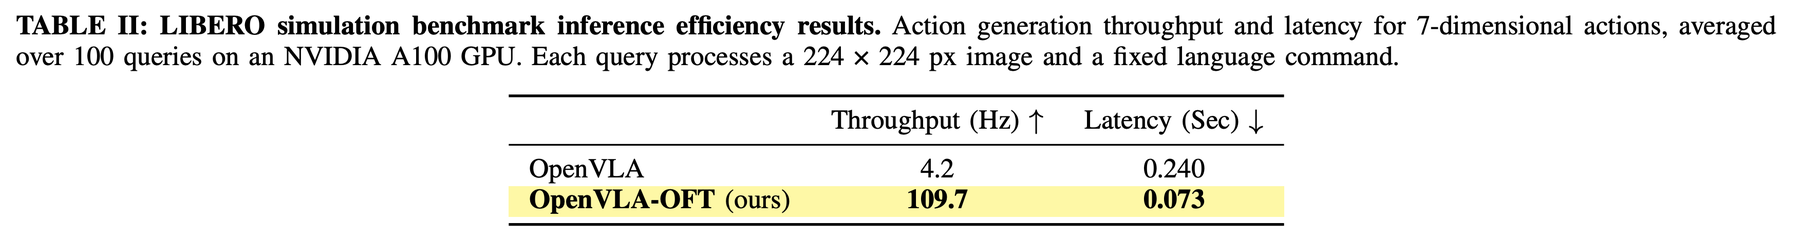
\includegraphics[width=0.9\textwidth]{figures/openvla_oft_efficiency.png}
\caption{OpenVLA-OFT 项目页给出的 LIBERO 推理效率结果（原表），在 NVIDIA A100 上测量。\figsrc{openvlaoft}}
\label{fig:oftefficiency}
\end{figure}
FAST~\cite{fast} 用离散余弦变换压缩动作序列，缩短自回归解码长度。ACT~\cite{act} 与 Diffusion Policy~\cite{diffpolicy} 引入的动作分块，本身也是一种“以一次推理换多步控制”的摊销手段。Dadu-Corki~\cite{corki} 进一步让模型预测近未来的轨迹而非单帧动作，以降低大模型的调用频率（第~\ref{sec:robot} 节）。这类方法改变的是负载本身，对任何硬件平台都有效。

\subsection{跨帧复用与 token 剪枝}

VLA 的前缀计算约占 85\% 的 MAC（第~\ref{sec:pi0profile} 节），而机器人连续两帧观测之间往往只有局部变化。VLA-Cache~\cite{vlacache} 利用这种时间连续性，识别相邻帧间变化很小的视觉 token 并复用其 KV，只对与任务相关、对环境敏感的 token 重算。据摘要，它在 LIBERO、SIMPLER 与真实机器人上取得最高约 1.7 倍的 CUDA 时延加速，控制频率提升 15\%，成功率损失可以忽略（方法见图~\ref{fig:vlacache}）\hw{NVIDIA GPU（CUDA 时延），具体型号本文未从可用来源读到}。
\begin{figure}[t]
\centering
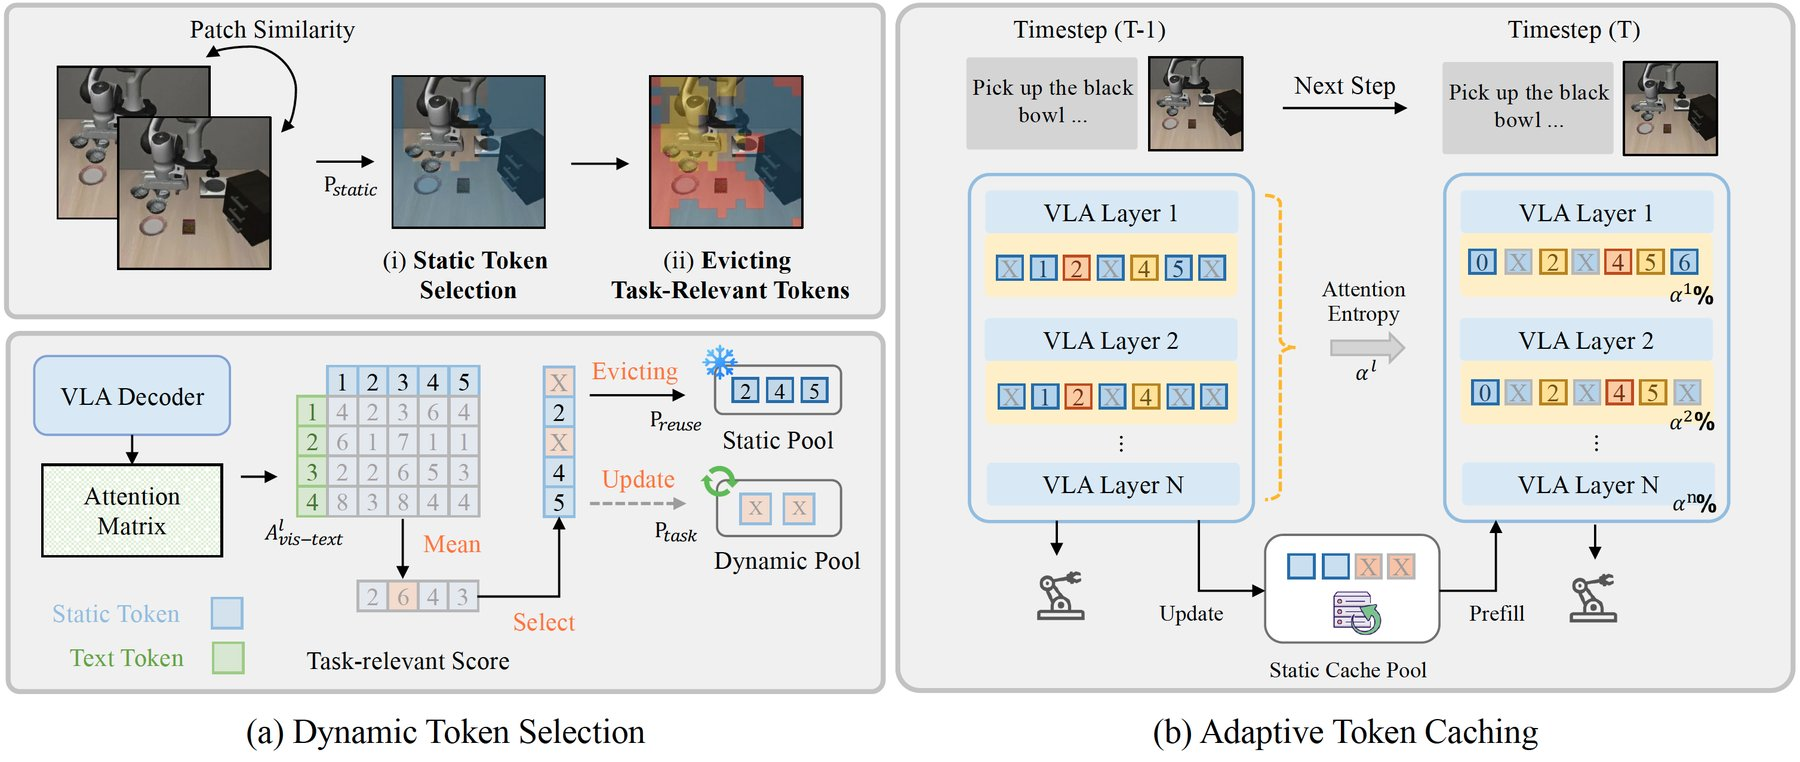
\includegraphics[width=0.95\textwidth]{figures/vlacache_method.jpg}
\caption{VLA-Cache 的方法：(a) 动态 token 选择——依据相邻帧的图块相似度选出静态 token，并依据注意力得分剔除与任务相关的 token；(b) 自适应 token 缓存——按层的注意力熵决定复用比例，把静态 token 的 KV 放入缓存池，在下一时间步预填充。\figsrc{vlacache}}
\label{fig:vlacache}
\end{figure}
视觉 Transformer 加速器中的自适应 token 剪枝（如 HeatViT~\cite{heatvit}，第~\ref{sec:fpga} 节）与之思路相通，只是后者作用于单帧内部。

\subsection{动态深度与早退}

DeeR-VLA~\cite{deervla} 观察到机器人控制中较容易的情境占多数，这些情境只需要较小的模型。它采用多出口结构，按预设的平均计算量、峰值计算量与显存约束决定激活多少层。在 CALVIN 基准上，它报告计算量降低 5.2 至 6.5 倍、GPU 显存降低 2 至 6 倍，且不损失性能。官方代码库说明其 CALVIN 评测在 8 块 V100 上运行（属于评测用途，而非部署平台）\hw{评测：8$\times$NVIDIA V100；以 CALVIN 仿真为基准}。动态深度对 GPU 友好，但会破坏静态调度的确定性，这一点在 FPGA 上需要权衡（第~\ref{sec:future} 节）。

\subsection{减少去噪或积分步数}

扩散与流匹配策略的步数是最直接的时延杠杆。Consistency Policy~\cite{consistencypolicy} 通过在预训练 Diffusion Policy 的轨迹上强制自一致性进行蒸馏，据摘要在 9 个仿真与真实任务上显著提高推理速度而不牺牲成功率，其动机正是“移动机械臂、四旋翼等平台无法搭载高端 GPU”（图~\ref{fig:cp}）；据检索，其演示在笔记本 GPU 上运行\hw{笔记本 GPU}。LightDP~\cite{lightdp} 面向移动设备压缩扩散 Transformer 策略并减少采样步数。据检索到的摘要信息，它在 iPhone 13 上分析了扩散策略的时延构成（扩散 Transformer 在 DP-T 中占总推理时间的 90\% 以上），并把 DP-T 与 MDT-V 中扩散 Transformer 的时延分别从 90.6~ms、22.25~ms 降至 2.72~ms、4.1~ms\hw{Apple iPhone 13}。
\begin{figure}[t]
\centering
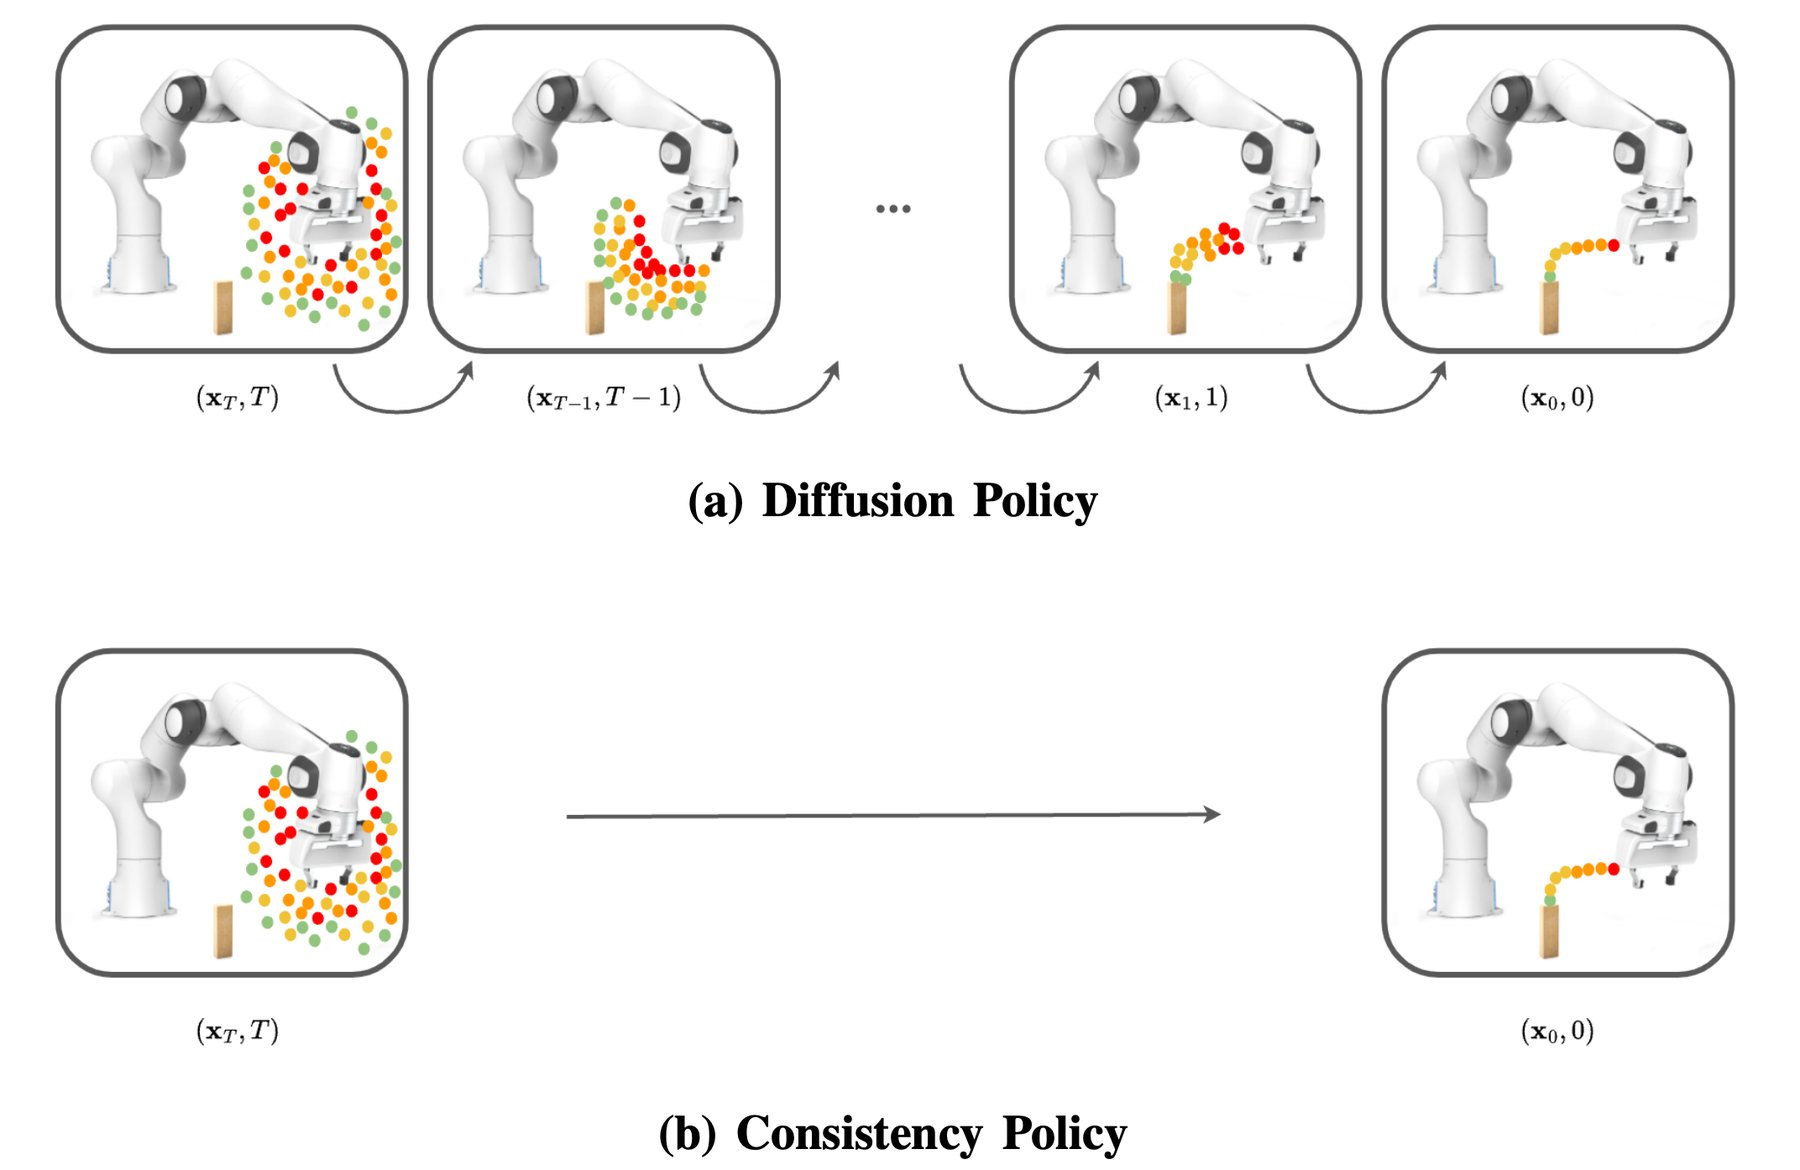
\includegraphics[width=0.6\textwidth]{figures/consistency_policy_teaser.jpg}
\caption{Diffusion Policy 与 Consistency Policy 的推理过程对比：前者从噪声 $(\mathbf{x}_T,T)$ 逐步去噪到 $(\mathbf{x}_0,0)$，后者一步完成映射。\figsrc{consistencypolicy}}
\label{fig:cp}
\end{figure}
这类方法表明，“减少积分或去噪步数”是生成式动作头端侧部署的通用手段，但通常需要额外的蒸馏或训练。

\subsection{量化}

\textbf{LLM 量化方法。} LLM.int8()~\cite{llmint8} 结合按向量量化与离群特征的混合精度分解，使 1,750 亿参数模型可以 INT8 推理而不降性能。SmoothQuant~\cite{smoothquant} 通过数学等价变换把激活中的离群值迁移到权重，使 W8A8 量化免训练且几乎无损，据摘要带来最高 1.56 倍加速与 2 倍内存节省（原理见图~\ref{fig:smoothquant}；其论文的 GPU 评测使用 NVIDIA A100）\hw{NVIDIA A100}。GPTQ~\cite{gptq} 基于近似二阶信息做逐层权重量化，可在约 4 GPU 小时内把 1,750 亿参数模型量化到 3 或 4 位。AWQ~\cite{awq} 观察到保护约 1\% 的显著权重即可大幅降低量化误差，并通过激活感知的按通道缩放实现低比特仅权重量化（图~\ref{fig:awq}）；其官方代码库以 RTX 4090 与 Jetson Orin 演示 TinyChat 边缘推理（W4A16 相对 FP16 分别快约 2.7 与 2.9 倍）\hw{RTX 4090、Jetson Orin}。
\begin{figure}[t]
\centering
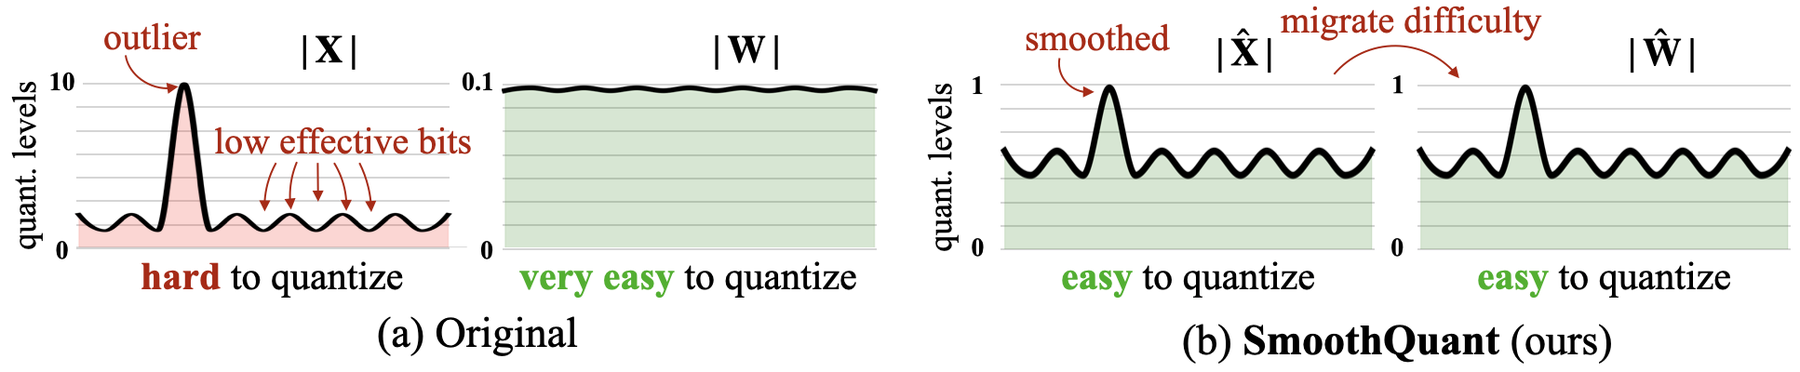
\includegraphics[width=0.95\textwidth]{figures/smoothquant_intuition.png}
\caption{SmoothQuant 的原理：(a) 激活中存在离群值、难以量化，而权重分布平坦、易于量化；(b) 通过数学等价的逐通道缩放把量化难度从激活迁移到权重，使二者都易于量化。\figsrc{smoothquant}}
\label{fig:smoothquant}
\end{figure}

\begin{figure}[t]
\centering
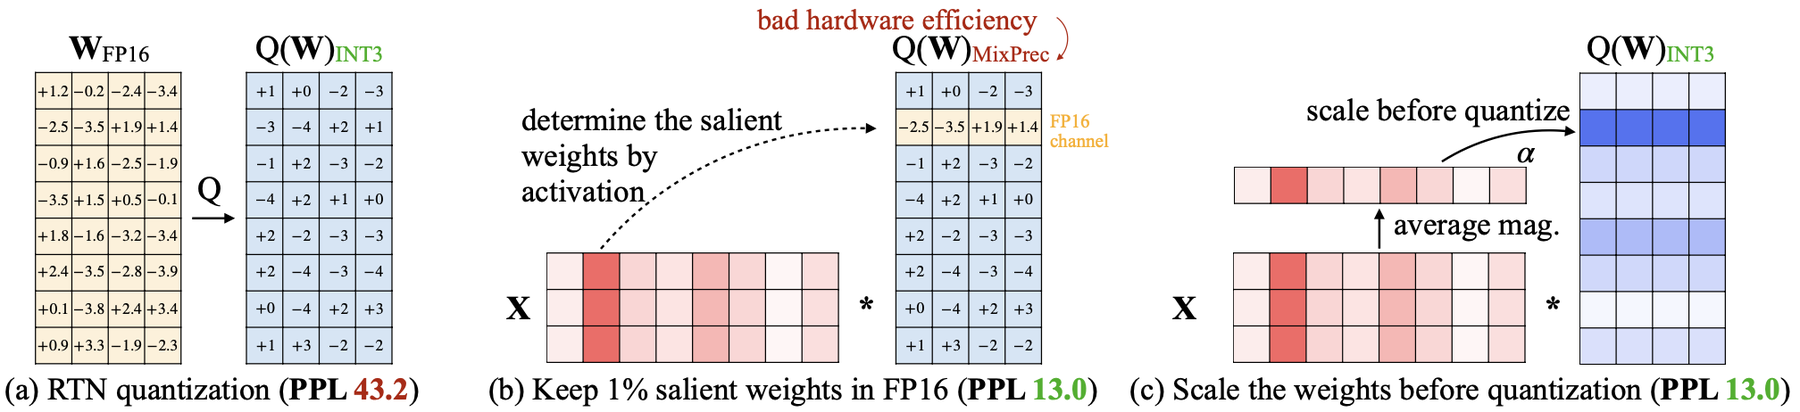
\includegraphics[width=0.95\textwidth]{figures/awq_overview.png}
\caption{AWQ 的原理：(a) 直接 RTN 量化到 INT3 导致困惑度大幅上升；(b) 以激活幅值判定并保留 1\% 的显著权重为 FP16 可恢复精度，但混合精度对硬件不友好；(c) 在量化前按激活幅值缩放权重，达到同等精度且保持统一位宽。\figsrc{awq}}
\label{fig:awq}
\end{figure}


\textbf{量化粒度的硬件代价。} 从硬件角度看，量化方案的代价不只取决于位宽，还取决于尺度的粒度与计算方式。按输出通道的权重尺度是静态的，可以离线计算并随权重一起存储，反量化时只需乘以一个列常数。按 token 的动态激活尺度则必须在运行时对每一行求最大绝对值，这是一个行归约操作，要求在量化之前看到整行数据。分组量化（每若干个元素共享一个尺度）进一步提高了精度，但使反量化需要在点积的中间插入尺度乘法，破坏了整数累加的连续性。块浮点可以看作分组量化的一种硬件友好形式：共享指数在块内对齐尾数后，点积可以在整数域中完成，只在块边界处理指数。对 FPGA 而言，这些粒度选择直接决定了向量通路的工作量与矩阵单元结果通路的复杂度，应与第~\ref{sec:nonlinear} 节讨论的非线性算子实现一起设计。

\textbf{VLA 专用量化。} 2025 至 2026 年出现了一批针对 VLA 的后训练量化工作，包括 QuantVLA~\cite{quantvla}、DA-PTQ~\cite{daptq} 与 HoloQ-VLA~\cite{holoq}。VLAQuantBench~\cite{vlaquantbench} 做了大规模闭环评测，据其摘要，在 W4 权重下再把激活量化到 8 位，在四个“模型—任务”组合上使成功率下降 18 至 40 个百分点，且 W4A4 下的结果强烈依赖于量化了哪些层。这些结论与案例项目“INT4 在全部非注意力 GEMM 上不可用”的实测结果（第~\ref{sec:case} 节）在方向上一致：VLA 的动作输出对低比特误差的敏感度高于语言任务。需要注意，这些工作多以仿真基准的成功率为指标，而案例项目以相对 fp32 的关节角误差为指标，两者不能直接换算。

\subsection{系统级表征与异步执行}

VLA-Perf~\cite{vlaperf}（图~\ref{fig:vlaperfoverview}）建立了 VLA 推理的解析性能模型，系统分析了模型规模、结构选择、长视频上下文、异步推理与双系统模型对时延的影响，以及端侧、边缘服务器与云端三种部署位置的取舍，给出 15 条设计要点。其官方代码库说明，建模覆盖数据中心 GPU（A100、H100、B100）、边缘 GPU（RTX 4090）与 Jetson 系列嵌入式设备（含 AGX Thor、AGX Orin 等）\hw{解析模型：A100/H100/B100、RTX 4090、Jetson 系列}。
\begin{figure}[t]
\centering
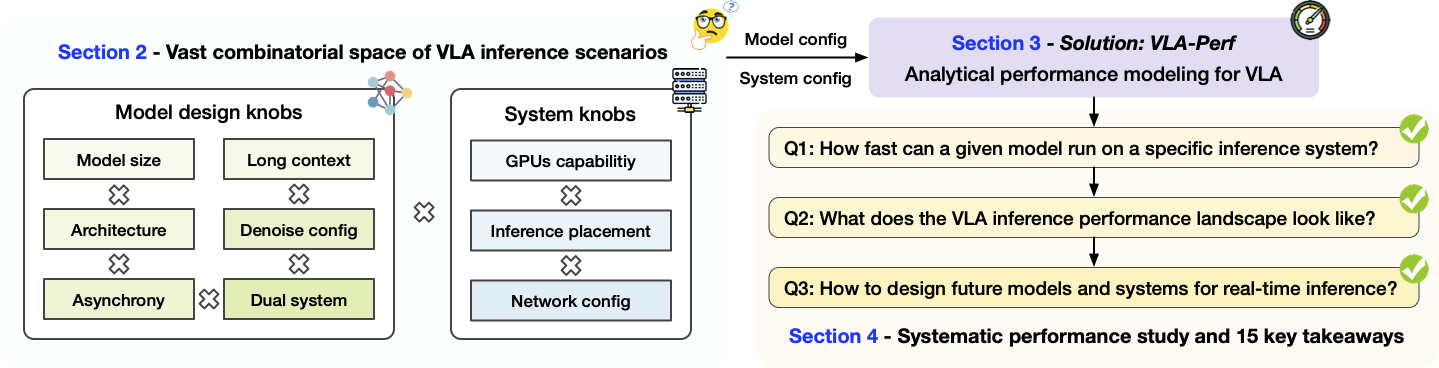
\includegraphics[width=0.95\textwidth]{figures/vlaperf_overview.png}
\caption{VLA-Perf 的问题设定：模型设计维度（规模、结构、长上下文、去噪配置、异步、双系统）与系统维度（GPU 能力、推理位置、网络配置）组合出的推理场景空间，以及其要回答的三个问题。\figsrc{vlaperf}}
\label{fig:vlaperfoverview}
\end{figure}

\begin{figure}[t]
\centering
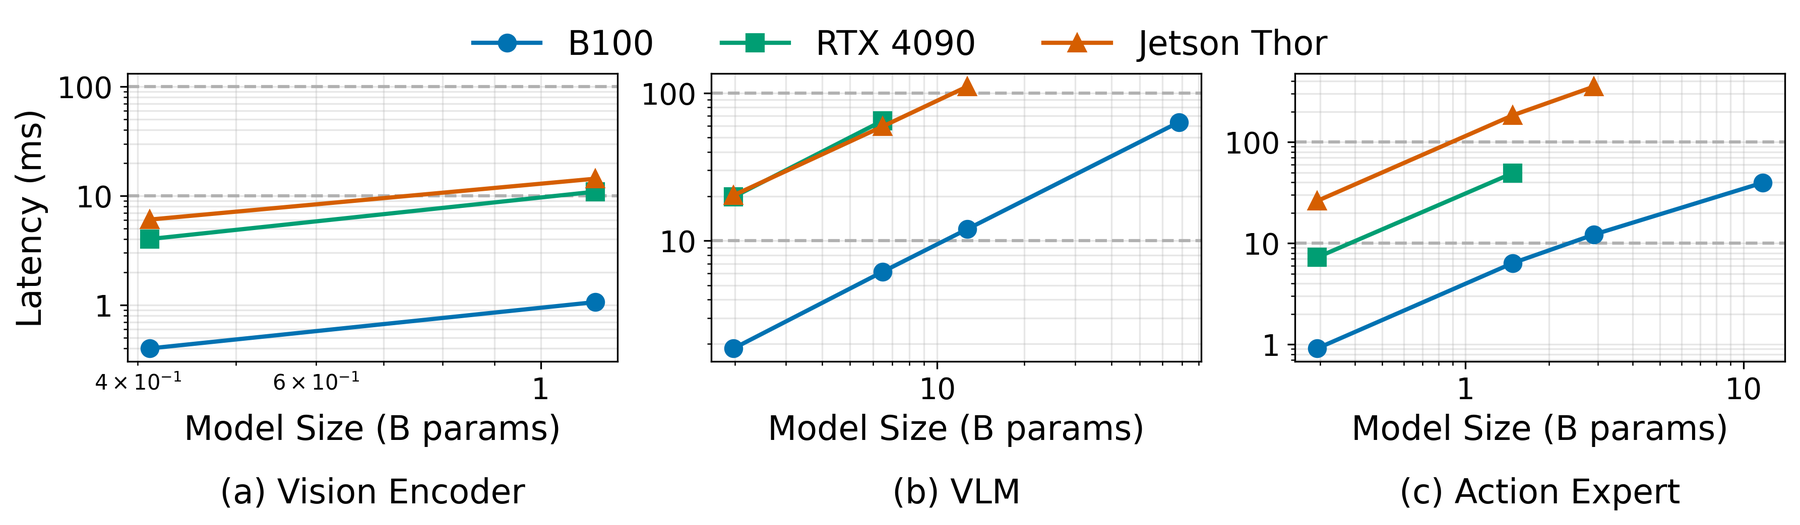
\includegraphics[width=0.95\textwidth]{figures/vlaperf_pi0_components.png}
\caption{VLA-Perf 解析模型给出的 \pizero{} 各组件时延随模型规模的变化：(a) 视觉编码器，(b) VLM，(c) 动作专家；平台为 B100、RTX 4090 与 Jetson Thor。\figsrc{vlaperf}}
\label{fig:vlaperfcomp}
\end{figure}
另一项跨加速器表征工作~\cite{xpuvla}\hw{CPU：Intel i7-11700；GPU：RTX 4090、Jetson Thor、Jetson AGX Orin；NPU：昇腾 310B/310P；XPU：Intel B60 Pro（据检索）} 提出了“成本—能耗—时间”排行榜，指出 VLA 推理存在两重串行性——VLM 与动作专家之间的流水线级串行，以及扩散过程内部的组件级串行——并据此提出两种免训练的加速方法；其结论之一是，在实时约束下，“规模合适”的边缘加速器可能比旗舰 GPU 更具成本与能耗优势。RTC~\cite{rtc} 则从执行侧放宽了时延约束（第~\ref{sec:loop} 节）；据检索，其真实机器人实验以 \pihalf{} 为基础策略、在单块 RTX 4090 上推理，并人为注入额外延迟以检验鲁棒性\hw{RTX 4090；双臂机器人}。

\subsection{部署位置与系统形态}

VLA-Perf~\cite{vlaperf} 讨论了 VLA 推理应当放在何处执行：机器人本体、边缘服务器还是云端。三种位置在时延构成上差别很大。本体推理没有网络时延，但受功耗与体积约束，算力最小；边缘服务器算力更大，但引入局域网往返；云端算力几乎不受限，但广域网时延与抖动难以保证。对于需要高频闭环的操作任务，网络时延与抖动本身就可能超出控制周期的预算，这使本体或近端推理成为首选。图~\ref{fig:vlaperfds} 是 VLA-Perf 对 \pizero{} 端到端时延的解析估计：Jetson Thor 本体推理约 52.6~ms；RTX 4090 边缘服务器经 10~Gb 以太网约 31.2~ms，经 4G 约 100.9~ms；B100 服务器经 10~Gb 以太网约 3.3~ms\hw{解析模型：Jetson Thor、RTX 4090、B100}。需要强调，这些是解析模型在其默认配置下的估计，与第~\ref{sec:case} 节案例在 Thor 上实测的 125.3~ms \tM{} 配置不同（输入 token 数、步数、数值格式与软件栈都可能不同），不能直接比较；但二者相差约 2.4 倍这一事实本身提示，实际软件栈与解析上界之间可能存在可观的空间。
\begin{figure}[t]
\centering
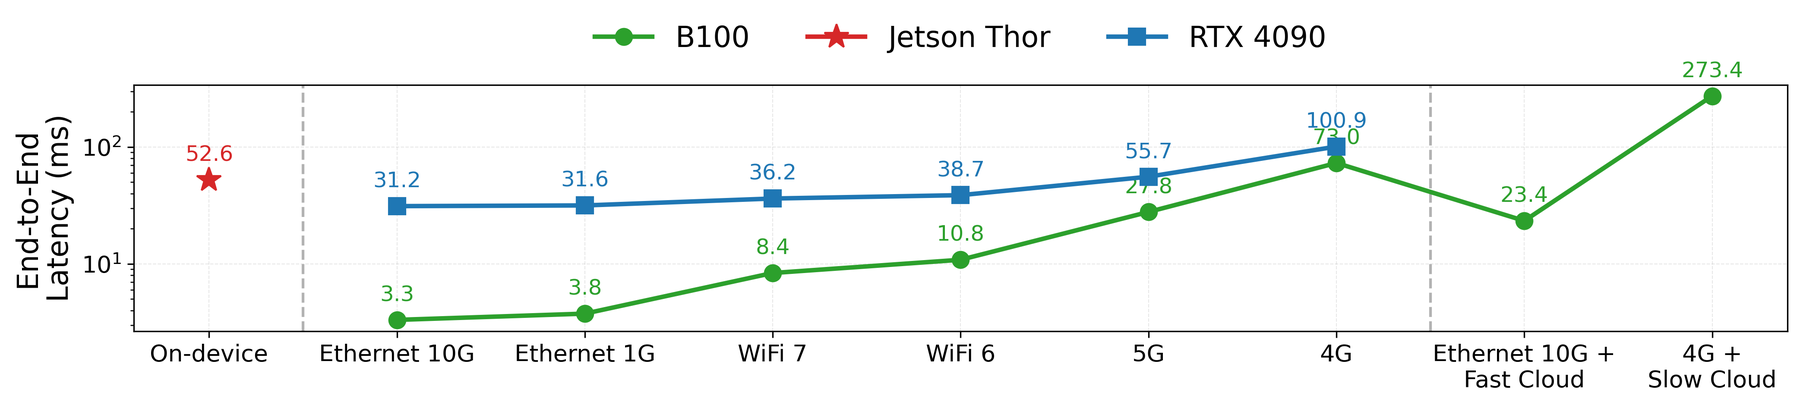
\includegraphics[width=0.95\textwidth]{figures/vlaperf_device_server.png}
\caption{VLA-Perf 解析模型给出的 \pizero{} 端到端时延：本体推理（Jetson Thor）与不同网络条件下的边缘/云端服务器推理（RTX 4090、B100）。\figsrc{vlaperf}}
\label{fig:vlaperfds}
\end{figure}


在本体推理中，系统形态又分为两种。一种是“单一 SoC”形态，如 Jetson 系列，CPU、GPU 与内存集成在同一封装中，数据不必跨越 PCIe；另一种是“主机 + 加速卡”形态，如第~\ref{sec:case} 节案例的 PCIe FPGA 卡，输入与输出需要经主机与 PCIe 传输。后者的主机开销（案例中约 47~ms/次调用）在百毫秒级的目标下已不可忽略。因此，FPGA 方案若要与 SoC 方案竞争，除了加速器内核本身，还需要考虑与传感器的直接连接（例如相机数据直接进入 FPGA）、减少主机参与等系统级设计。这类“把加速器放在数据通路上”的做法恰是 FPGA 的传统强项，但在 VLA 部署文献中尚未见系统讨论。

\subsection{小结}

通用平台路线的优化以算法与软件为主，硬件是给定的。上述收益（约 26 倍、1.7 倍、5 至 6 倍等）大多与硬件平台正交，可以叠加到 FPGA 方案上。这也意味着，FPGA 方案与 GPU/SoC 的比较必须在同一算法版本（相同步数、相同 token 数、相同量化粒度）下进行，否则没有意义。第~\ref{sec:case} 节案例与 Thor 的对照满足这一点：同一个 \pizero{} chunk，只是数值格式不同（W8A8 对 bf16）。

从体系结构的角度回看本节，可以把通用平台上的 VLA 优化归纳为三个层次：改变“算什么”（动作表示、步数、token 数），改变“算多少”（动态深度、剪枝、复用），以及改变“怎么算”（量化、融合、异步执行）。前两个层次减少的是负载本身，第三个层次提高的是执行效率。FPGA 方案的独特空间主要在第三个层次：它可以为特定负载定制数据通路、数值格式与存储层次，并提供确定性的执行；而前两个层次的收益，FPGA 方案应当与 GPU 方案同等地吸收，否则比较就失去了公平性。

%======================================================================
\section{FPGA 上的 Transformer 与 LLM 加速}\label{sec:fpga}
%======================================================================

本节按时间与负载类型梳理 FPGA 上的 Transformer 相关加速工作，并讨论对 VLA 部署有直接意义的器件、数值格式、编译栈与系统先例。已有综述从更广的角度覆盖了 LLM 的硬件加速~\cite{survey_llmhw,survey_llmhw2} 与 FPGA 上的 Transformer 推理部署~\cite{survey_fpga_tf}；本节的侧重点是与 VLA 负载特征相关的设计选择。

\subsection{早期的 Transformer 与注意力加速}

FTRANS~\cite{ftrans} 是较早的 FPGA Transformer 加速工作，采用增强的块循环矩阵表示压缩权重，据摘要把模型大小降低最多 16 倍，相对 CPU 取得 27.07 倍性能与 81 倍能效提升，相对 GPU 能效提升最高 8.80 倍。据检索到的论文正文，其实现平台为 Xilinx Virtex UltraScale+ VCU118 板卡，以 SDx 2017.1 做高层次综合，报告约 170~GOPS 与 6.8~GOPS/W\hw{Xilinx VCU118（Virtex UltraScale+）；对照：CPU、GPU}。它代表了“算法级压缩 + 专用数据通路”的早期路线。

在 ASIC 方向，一系列工作专门针对注意力。A$^3$~\cite{a3}\hw{ASIC 设计} 观察到注意力在语义上是一种基于内容的检索，大部分计算最终不被使用，据此以算法近似与硬件专用化结合加速注意力。ELSA~\cite{elsa}\hw{ASIC 设计} 提出一种高效过滤“不太可能影响输出的关系”的近似方案，降低自注意力的计算量。SpAtten~\cite{spatten} 通过级联的 token 剪枝与 head 剪枝减少注意力的计算与访存，并设计高吞吐的 top-$k$ 排序引擎与“先取高位、置信度低时再取低位”的渐进量化；据摘要它把 DRAM 访问量平均降低 10.0 倍，相对 A$^3$ 加速 1.6 倍，相对 TITAN Xp GPU 与 Xeon CPU 分别加速 162 倍与 347 倍（级联剪枝示意见图~\ref{fig:spatten}）\hw{ASIC 设计；对照：A$^3$、MNNFast、TITAN Xp GPU、Xeon CPU}。
\begin{figure}[t]
\centering
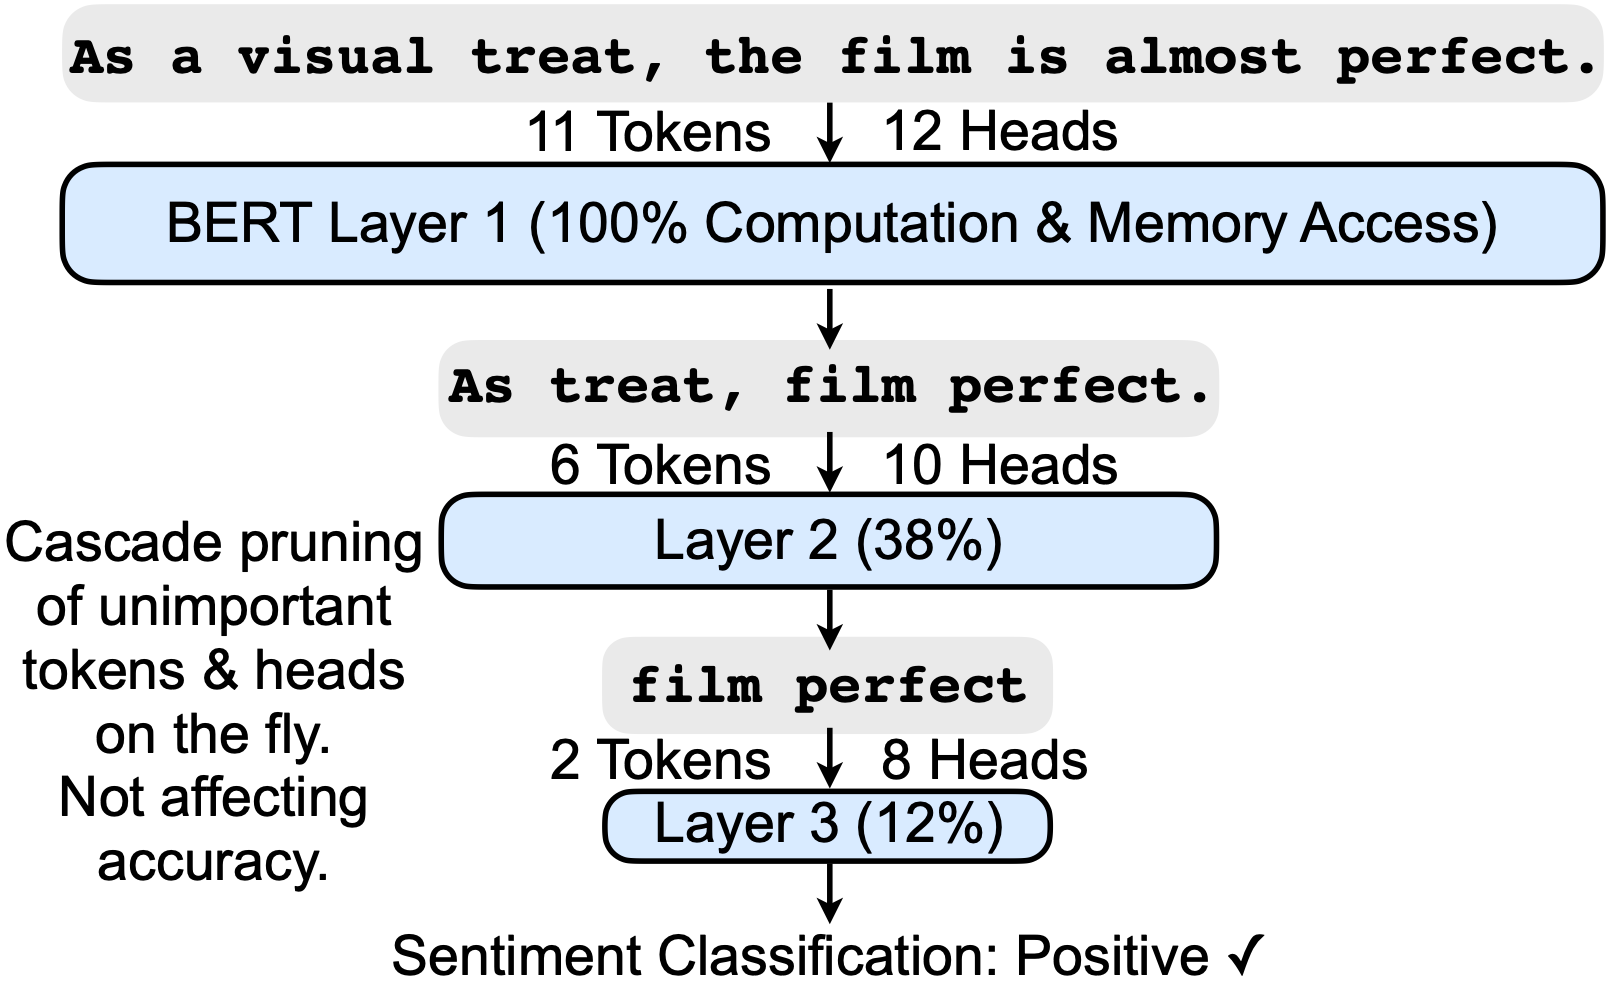
\includegraphics[width=0.5\textwidth]{figures/spatten_cascade_pruning.png}
\caption{SpAtten 的级联 token 与 head 剪枝示意：以 BERT 情感分类为例，逐层在运行时剪去不重要的 token 与 head，后续层的计算与访存随之减少。\figsrc{spatten}}
\label{fig:spatten}
\end{figure}
这类工作的着眼点是长序列注意力。对 \pizero{} 而言，前缀只有 525 个 token，注意力的 MAC 占比很低，其主要借鉴意义在于“对视觉 token 做运行时剪枝”的思想。

\subsection{视觉 Transformer 加速}

VLA 的视觉编码器通常是视觉 Transformer（ViT），因此 ViT 加速工作与 VLA 前缀的一部分直接相关。Auto-ViT-Acc~\cite{autovitacc} 提出面向 FPGA 的混合方案量化框架，据摘要相对 32 位浮点基线 FPGA 加速器把 DeiT-base 的帧率提升约 5.6 倍，ImageNet 精度下降 0.71\%\hw{Xilinx ZCU102，150~MHz（据检索到的论文正文）}。HeatViT~\cite{heatvit} 在嵌入式 FPGA 上实现图像自适应的 token 剪枝：它把非信息 token 打包为一个 token 而不是直接丢弃，在 ZCU102 上相对无剪枝的 16 位基线加速器取得 3.46 至 4.89 倍加速\hw{Xilinx ZCU102（嵌入式 FPGA）}。ViTCoD~\cite{vitcod} 利用 ViT 输入 token 数固定的特点，把注意力图剪枝并极化为稠密与稀疏两种固定模式，再以专用加速器协调两类负载（图~\ref{fig:vitcod}、图~\ref{fig:vitcodarch}）。其加速器以模拟器评估，官方代码库中的 FLOPs 与时延剖析则在 NVIDIA Jetson TX2 上测量\hw{专用加速器（模拟器评估）；剖析平台：Jetson TX2}。
\begin{figure}[t]
\centering
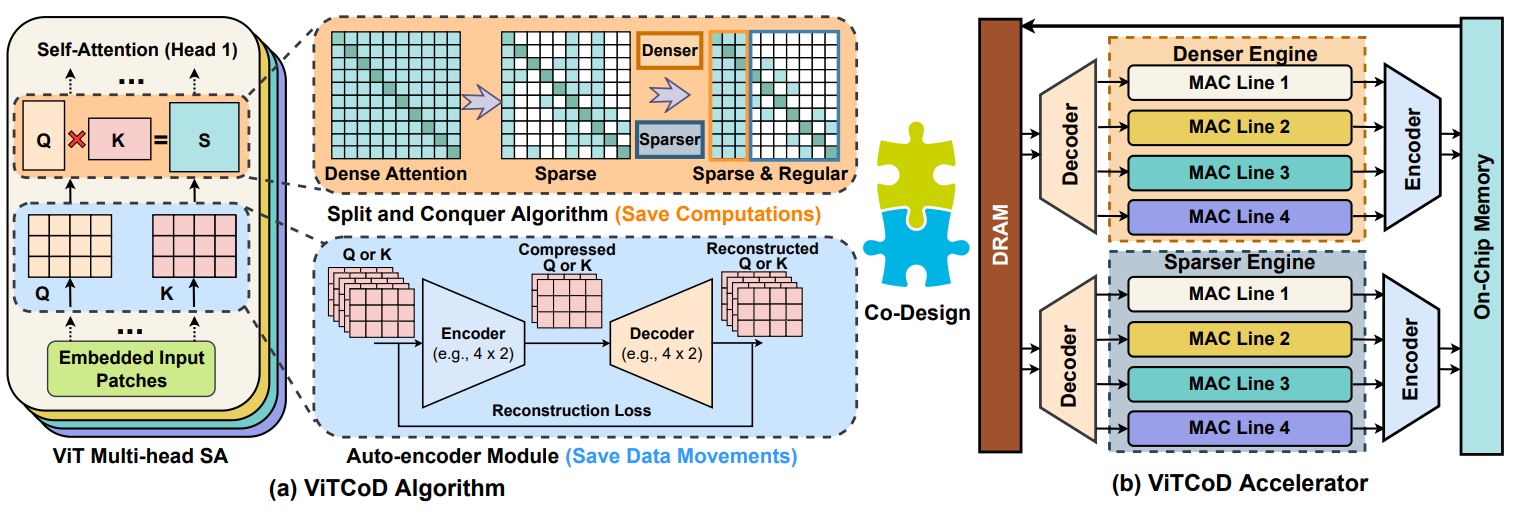
\includegraphics[width=0.95\textwidth]{figures/vitcod_overview.png}
\caption{ViTCoD 的算法与加速器协同设计：(a) 算法侧把注意力图划分为较稠密与较稀疏两类固定模式，并以自编码器压缩 Q/K 以减少数据搬运；(b) 加速器侧以“较稠密引擎”与“较稀疏引擎”分别处理两类负载，片上集成编码器与解码器。\figsrc{vitcod}}
\label{fig:vitcod}
\end{figure}

\begin{figure}[t]
\centering
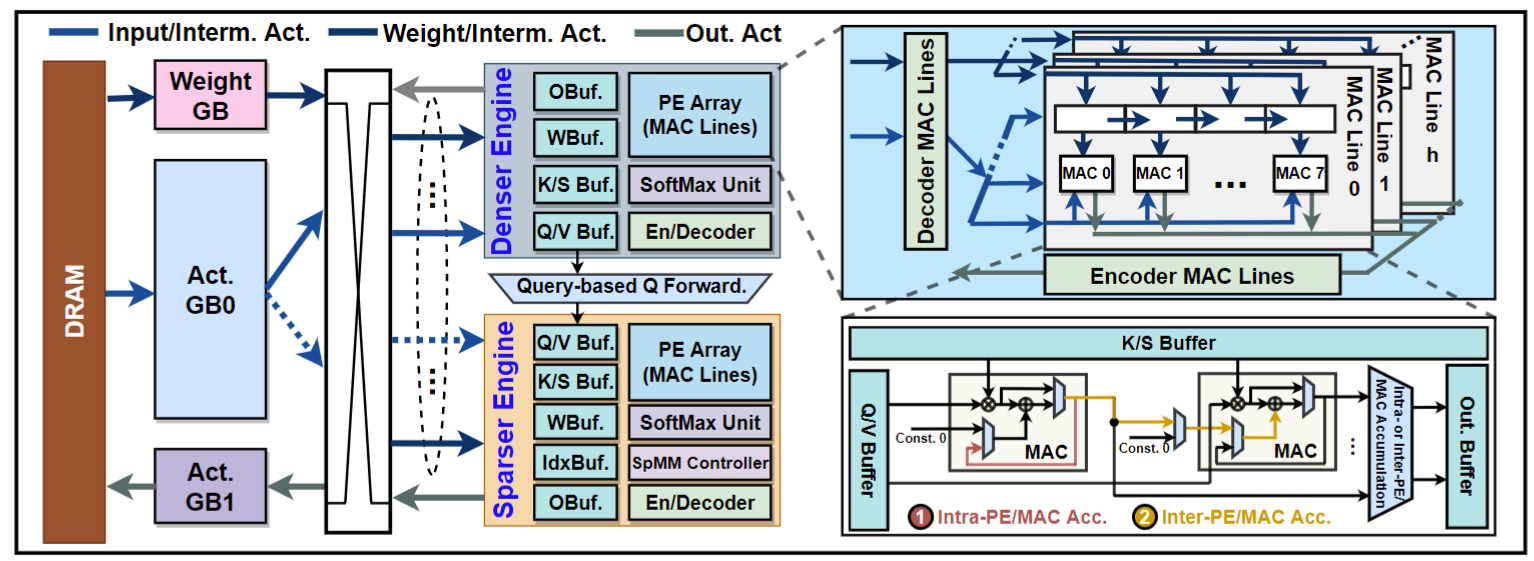
\includegraphics[width=0.9\textwidth]{figures/vitcod_arch.png}
\caption{ViTCoD 加速器的微结构：权重与激活全局缓冲经交叉开关连接“较稠密引擎”与“较稀疏引擎”，二者各含 MAC 行阵列、Softmax 单元与编解码器；右下为 PE 内与 PE 间累加的两种数据流。\figsrc{vitcod}}
\label{fig:vitcodarch}
\end{figure}
这些工作都利用了 ViT “token 数固定”的特点，这一点同样适用于 VLA 的视觉前缀；但它们大多只处理单帧，未利用机器人观测的帧间连续性。

\subsection{LLM 推理加速}

\textbf{DFX~\cite{dfx}（MICRO 2022）} 是由 4 块 Alveo U280 组成的多 FPGA 设备，端到端执行 GPT-2 的摘要（预填充）与生成（解码）两个阶段。它采用模型并行与“模型—硬件感知”的数据流，计算核执行自定义指令，用满 HBM 的所有通道，板间以 QSFP 组成环网。据摘要，它相对 4 块 V100 取得 5.58 倍加速与 3.99 倍能效\hw{4$\times$Xilinx Alveo U280（HBM）；对照：4$\times$NVIDIA V100}。DFX 的启示在于“自定义指令 + 端到端执行全部算子”：非线性算子不留给主机。

\textbf{FlightLLM~\cite{flightllm}（FPGA 2024）} 提出面向 LLM 的完整映射流程，平台为 Alveo U280。三项关键技术是：用于支持多种稀疏模式的可配置稀疏 DSP 链；解码阶段激活常驻片上并支持混合精度，以提升有效带宽；长度自适应编译，以降低不同序列长度下的编译开销。据摘要，在 batch 为 1 的 LLaMA2-7B 上，它相对 NVIDIA V100S（vLLM 与 SmoothQuant）取得 6.0 倍能效与 1.8 倍成本效率；据检索到的论文正文，它在 Versal VHK158 上达到约 92.5~tokens/s，吞吐约为 A100 的 1.2 倍\hw{Xilinx Alveo U280 与 Versal VHK158；对照：V100S、A100}。FlightLLM 与本文案例在思想上最接近：两者都利用硬核级联组织矩阵阵列，并依赖完整的编译流程；区别在于 FlightLLM 面向 $M=1$ 的解码，利用 HBM 与稀疏性，不涉及多步迭代的动作头。

\textbf{Chen 等~\cite{chen2024trets}（ACM TRETS）} 研究模型专用的空间加速：为特定算子或层专门化硬件单元，单元之间以数据流直连，尽量减少片外访问。其核心贡献是一个预测空间加速器性能的解析模型与一套可组合、可复用的 HLS kernel 库。在 U280 上，据摘要，BERT 相对此前 FPGA 加速器最高加速 13.4 倍；GPT 的预填充相对 DFX 加速 2.2 倍，解码相对 A100 加速 1.9 倍、能效提高 5.7 倍\hw{AMD Alveo U280；对照：DFX、NVIDIA A100}。该文讨论的空间（层间流水）与时间复用（单一阵列逐层执行）之间的取舍，正是 VLA 双形态负载需要面对的问题。

\textbf{HLSTransform~\cite{hlstransform}} 用高层次综合（High-Level Synthesis，HLS）在 Virtex UltraScale+ VU9P 上实现 Llama 2 推理。据摘要，每 token 能耗相对 Xeon CPU 降低最多 12.75 倍、相对 RTX 3090 降低 8.25 倍，速度约为 RTX 3090 的 0.53 倍\hw{Xilinx VU9P；对照：Intel Xeon E5-2686 v4、NVIDIA RTX 3090}。“能效优于 GPU、绝对速度不及 GPU”是 FPGA LLM 工作中相当普遍的格局。

\textbf{EdgeLLM~\cite{edgellm}} 是 CPU-FPGA 异构的边缘 LLM 加速器，平台为带 HBM 的 VCU128。它采用混合精度处理单元阵列与分组脉动结构，注意力部分用 FP16$\times$FP16，前馈网络用 FP16$\times$INT4，并以统一的数据形状使不同算子无需数据重排\hw{Xilinx VCU128（带 HBM）+ 主机 CPU}。它是“按层类型分配精度”的代表，与本文案例“均匀 W8A8 / 均匀 INT4”两种方案形成对照。

\textbf{近期工作。} 面向边缘 FPGA 的三值 LLM 加速器 TeLLMe v2~\cite{tellme} 以查表矩阵乘同时支持预填充与解码；据检索，TeLLMe 系列在 AMD Kria KV260（Zynq UltraScale+ XCK26，250~MHz）上实现，报告解码约 9.51~tokens/s、预填充时延约 0.55~s\hw{AMD Kria KV260}。SpeedLLM~\cite{speedllm}（HPDC 2025）在 Alveo U280 上针对 TinyLlama 做数据流并行、存储复用与算子融合，据摘要相对传统 TinyLlama 实现最高快 4.8 倍、能耗低 1.18 倍\hw{Xilinx Alveo U280}。这些工作延续了“低比特 + 带宽优化”的思路，但目标负载仍是语言模型解码。

\textbf{各工作对 VLA 的适用性。} 上述 LLM 加速工作各自针对的负载形态不同，迁移到 VLA 时的适用程度也不同。DFX 与 Chen 等的工作同时处理了预填充与解码，其“端到端执行全部算子”与“空间/时间复用取舍”的经验可以直接借鉴，但它们使用多块或大型带 HBM 的器件，与机器人端侧的功耗与体积约束不同。FlightLLM 与 EdgeLLM 的核心优化针对 $M=1$ 的解码，其稀疏 DSP 链与混合精度可以用于 VLA 的前缀与动作头，但“解码阶段激活常驻片上”在 VLA 中需要改为“前缀 KV 与专家权重常驻”。HLSTransform 展示了 HLS 流程的可达性，但其绝对速度约为高端 GPU 的一半，在 VLA 的时延约束下需要进一步提升。三值与低比特方案（如 TeLLMe~\cite{tellme}）在语言模型上可行，但在对量化更敏感的 VLA 上是否可用尚无证据，本文案例的 INT4 结果对此提出了警示。

\subsection{AI 优化器件上的阵列组织}

\textbf{Stratix 10 NX。} 如第~\ref{sec:bg} 节所述，其 AI Tensor Block 以 INT8/INT4 为基础精度并支持块浮点，前馈数据通路即使用满全部张量块也能在中速等级器件上以 500~MHz 以上收敛时序~\cite{s10nx_fpga21,s10nx_trets}。Boutros 等~\cite{s10nx_fpt} 的实测对比表明，其张量块的 INT8 峰值约 143~TOPS，但实际可达性能主要取决于张量单元利用率与系统开销；相对常规 DSP 的 FPGA 平均提升 3.5 倍\hw{Intel Stratix 10 NX；对照：NVIDIA T4、V100}。

\textbf{Versal AI Engine。} CHARM~\cite{charm}（FPGA 2023）观察到，把 BERT 中尺寸较小的矩阵乘层放在 Versal ACAP 上一个庞大的单体矩阵乘加速器上执行，只能达到理论峰值的不到 5\%；它据此提出组合多个异构矩阵乘加速器，并发服务不同尺寸的层。该文给出的平台背景为 400 个 AIE、1~GHz、fp32 峰值约 6.4~TFLOPs。图~\ref{fig:charmversal} 摘自作者的报告幻灯片，展示了 Versal 的编程模型：AIE 阵列与可编程逻辑之间约 1.2~TB/s，而 DDR4 经 NoC 约 25.6~GB/s——片外带宽与片上带宽相差近两个数量级，这正是小矩阵在单体加速器上利用率低的根源之一；图~\ref{fig:charmframework} 为 CHARM 的自动化框架\hw{AMD Versal VCK190；官方代码库亦支持 VCK5000}。
\begin{figure}[t]
\centering
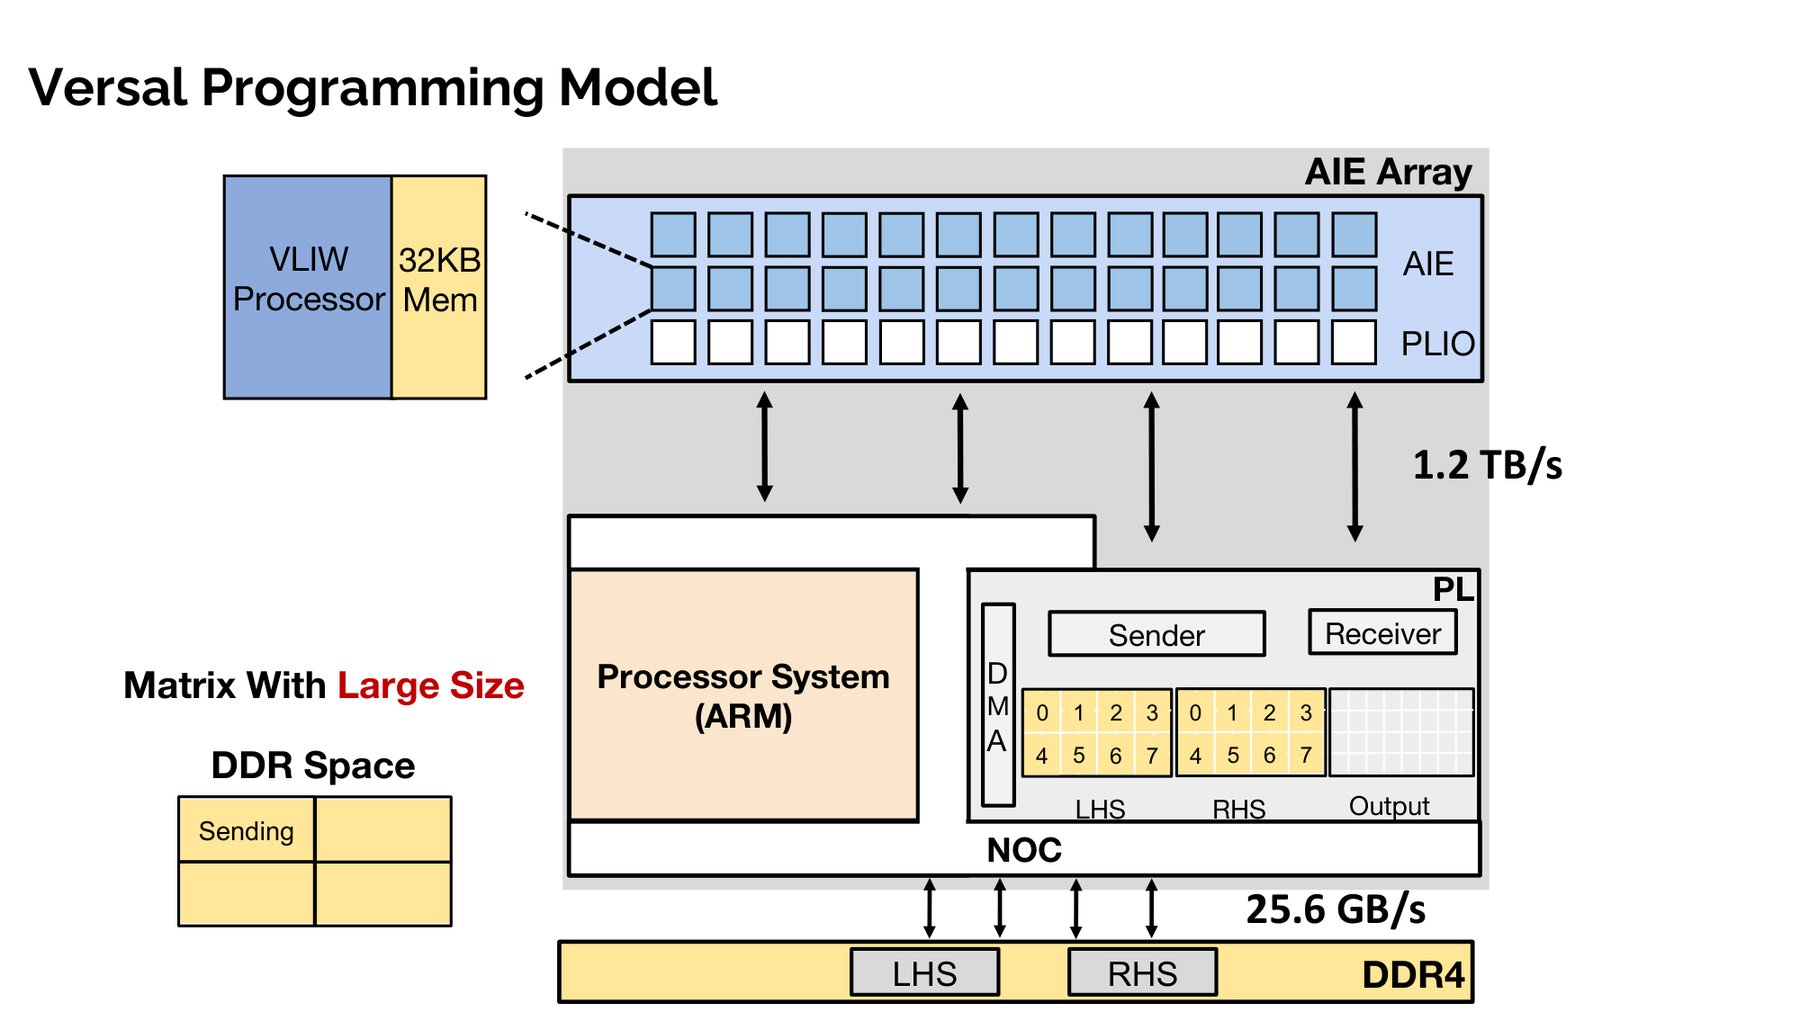
\includegraphics[width=0.7\textwidth]{figures/charm_versal_model.jpg}
\caption{Versal 编程模型（摘自 CHARM 作者报告幻灯片）：由 VLIW 处理器与 32~KB 本地存储组成的 AIE 阵列，经 PLIO 与可编程逻辑相连（约 1.2~TB/s），可编程逻辑经 NoC 访问 DDR4（约 25.6~GB/s）。\figsrc{charm}}
\label{fig:charmversal}
\end{figure}

\begin{figure}[t]
\centering
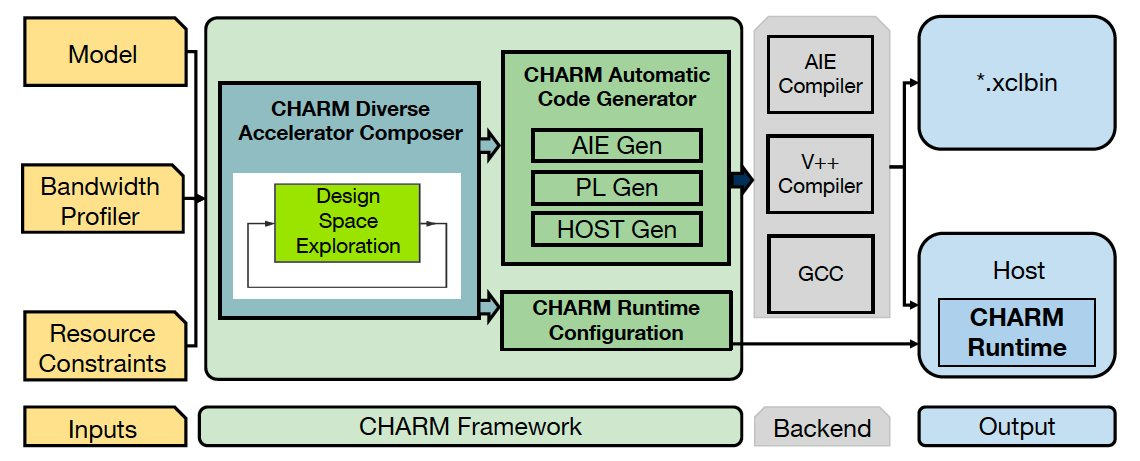
\includegraphics[width=0.8\textwidth]{figures/charm_framework.jpg}
\caption{CHARM 框架：以模型、带宽剖析与资源约束为输入，经多样加速器组合器（设计空间探索）与自动代码生成器（AIE/PL/HOST）生成比特流与主机运行时。\figsrc{charm}}
\label{fig:charmframework}
\end{figure}
SSR~\cite{ssr}（FPGA 2024）进一步在 VCK190 上把空间并行与顺序执行混合，给出时延—吞吐的帕累托前沿，据摘要相对 A10G 平均吞吐提升 2.53 倍\hw{AMD Versal VCK190；对照：NVIDIA A10G、ZCU102、U250}。这两项工作对 VLA 最直接的意义是：\emph{不同形状的 GEMM 需要不同形状的阵列}。CHARM 的“不到 5\%”与 VLA 中“前缀 $M\approx525$ 与专家 $M=51$ 共享同一阵列”面对的是同一个问题。

\textbf{Speedster7t。} 其 MLP 阵列、二维 NoC 与 GDDR6 接口~\cite{achronix} 构成了本文案例的平台（第~\ref{sec:case} 节）。与 U280 的 HBM + AXI 互连、Versal 的 AIE 阵列 + 可编程逻辑相比，Speedster7t 的特点是“硬核级联 + 硬化 NoC 直达 GDDR6”，更适合由多个独立单元各自访存的组织方式。

\subsection{片上存储层次的组织}

在权重无法全部常驻的前提下，片上存储的组织方式决定了片外带宽能否被充分利用。常见的手段有三种。其一是\emph{双缓冲}（乒乓缓冲）：计算单元使用一块缓冲区时，另一块缓冲区从外存装入下一批数据，使装入与计算重叠。其二是\emph{地址条带化}：把一个张量按块分散到多个外存通道，使多个计算单元的并发访问均匀分布在各通道上，避免热点；DFX~\cite{dfx} “用满 HBM 全部通道”的设计与案例项目的“条带化 GDDR6 地址映射”都属于此类。其三是\emph{分级存储}：小容量、高带宽的寄存器或分布式 RAM 存放当前操作数，较大的块 RAM 存放权重分块或激活行，外存存放全部权重。

对 VLA，还有一个与 LLM 不同的考虑：前缀 KV 与动作专家权重在一个 chunk 内被重复使用，它们应当在分级存储中获得比前缀权重更高的优先级。这需要编译器能够在全局范围内分析数据的重用距离，而不是逐层独立地分配缓冲。HeteroFlow~\cite{heteroflow} 的数据放置原语与 Allo~\cite{allo} 的存储定制原语为这类全局分析提供了编程模型层面的支持，但尚未见到把它们用于 VLA 这类“一次性前缀 + 多次重复”负载的工作。

\subsection{数值格式}

块浮点（Block Floating Point，BFP）让一组元素共享指数，元素本身用窄位宽尾数，在接近整数运算的硬件成本下保留一定动态范围。MSFP~\cite{msfp}（NeurIPS 2020）是微软 Brainwave 生产系统使用的块浮点族\hw{微软云端定制推理硬件（Brainwave，FPGA）}，据摘要在不修改模型拓扑的前提下，以低于 bf16 约 3 倍、低于 INT8 约 4 倍的成本达到相当精度，精度影响小于 1\%。MX~\cite{mx} 规范在此基础上定义了块大小、共享尺度与窄位宽元素三要素，给出 MXFP8、MXFP6、MXFP4 与 MXINT8 四种格式（其参考实现中线性层的量化与舍入位置见图~\ref{fig:mx}），并报告在二十余个基准上可作为 FP32 的直接替代，还首次在亚 8 位权重、激活与梯度下训练生成式语言模型。Stratix 10 NX 的张量块原生支持 Block FP16 与 Block FP12~\cite{s10nx_fpga21}；面向机器人学习，已有工作设计了支持 MX 的精度可伸缩硬件~\cite{mxrobot}\hw{TSMC 16~nm ASIC 综合，500~MHz（据检索）}。
\begin{figure}[t]
\centering
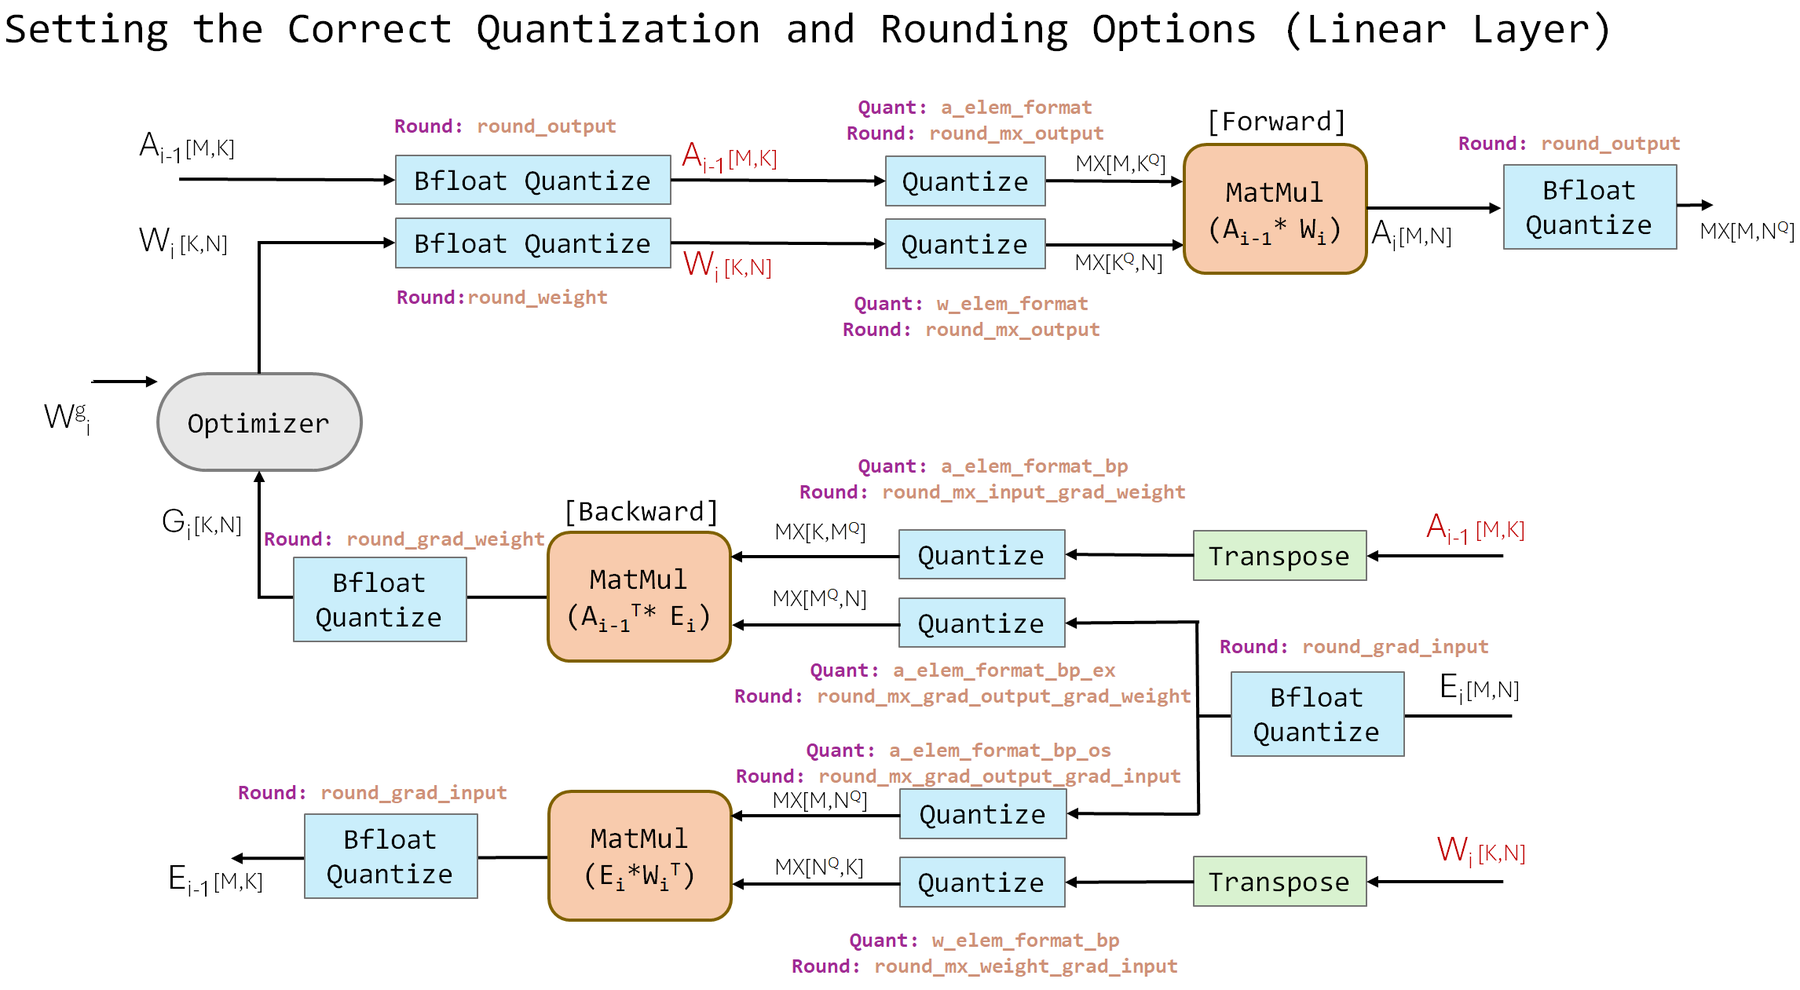
\includegraphics[width=0.85\textwidth]{figures/mx_linear_quant.png}
\caption{MX 参考实现（microxcaling）中线性层前向与反向传播的量化与舍入选项：矩阵乘的输入在进入 MatMul 前先做 bfloat 量化，再按 MX 元素格式量化。\figsrc{mx}}
\label{fig:mx}
\end{figure}
在 VLA 对精度敏感的前提下，块浮点是“以接近 INT8 的成本换取更好精度”的主要候选，第~\ref{sec:case} 节案例的 BFP8 探索提供了一个具体数据点。

\subsection{编译栈}

FPGA 上的神经网络编译栈大致经历了三代。第一代以数据流生成器为主：FINN~\cite{finn}（FPGA 2017）\hw{Xilinx ZC706} 为二值化网络生成异构流式架构，按用户给定的吞吐需求为每层裁剪计算资源；hls4ml~\cite{hls4ml} 以 HLS 为基础，面向粒子物理触发系统生成超低时延的网络推理电路（流程见图~\ref{fig:hls4ml}）\hw{大型强子对撞机触发系统中的 FPGA}。
\begin{figure}[t]
\centering
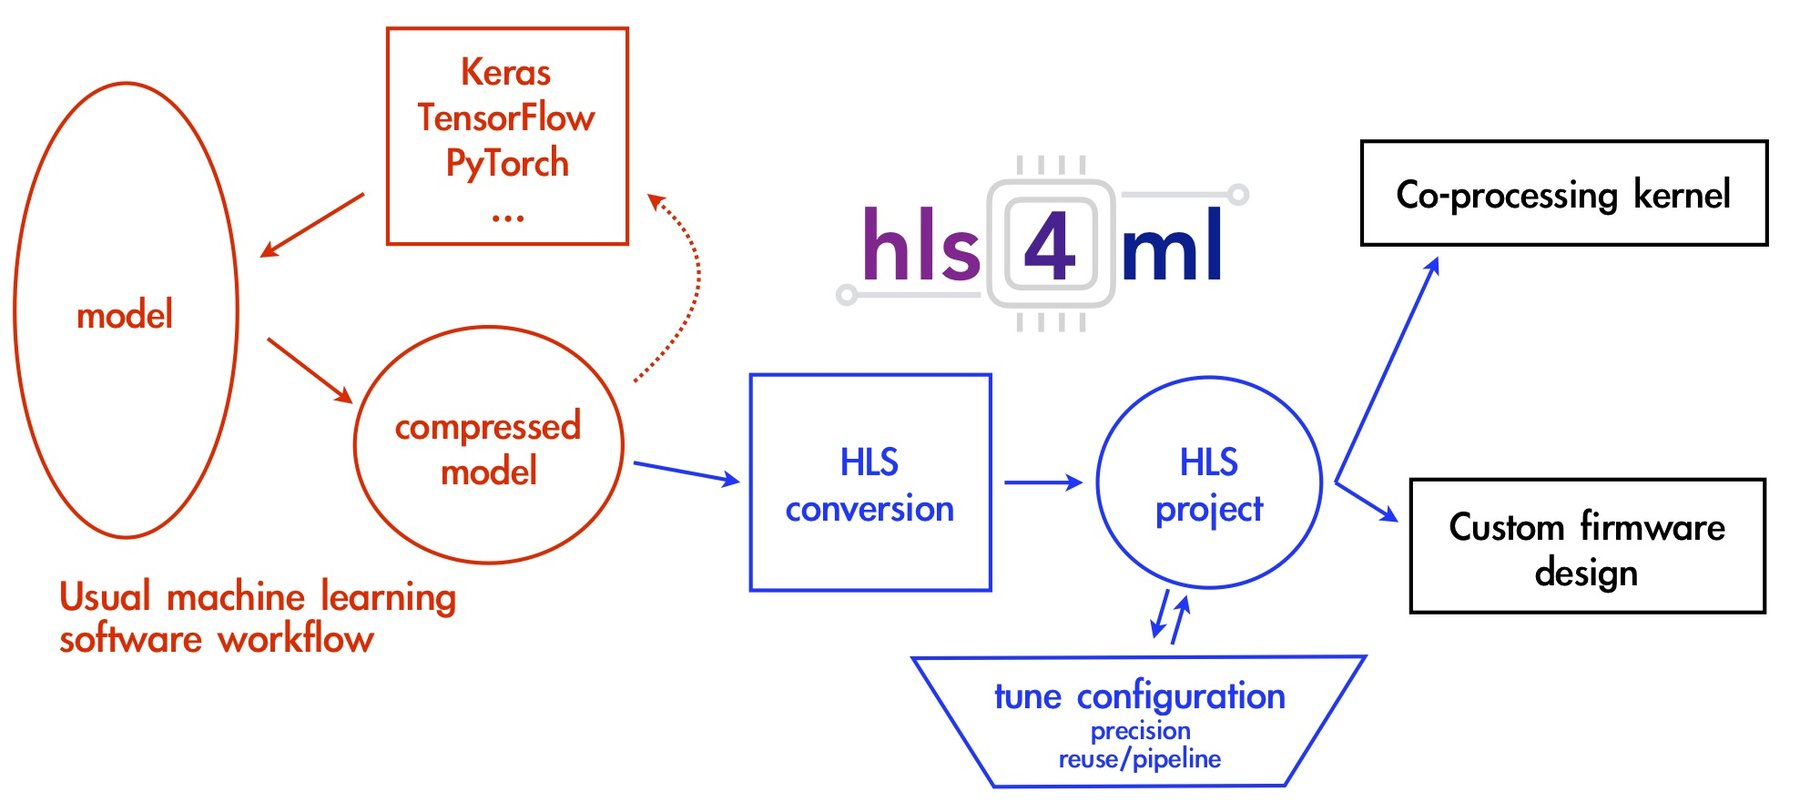
\includegraphics[width=0.7\textwidth]{figures/hls4ml_flow.jpg}
\caption{hls4ml 的设计流程：常规机器学习框架训练并压缩的模型经 HLS 转换生成 HLS 工程，调节精度与复用/流水配置后，输出协处理 kernel 或定制固件。\figsrc{hls4ml}}
\label{fig:hls4ml}
\end{figure}
这两者都假设权重可以全部常驻片上，适用于小模型。第二代以“解耦的硬件定制”为特征：HeteroFlow~\cite{heteroflow}（FPGA 2022）构建于 HeteroCL 之上，用统一的 \texttt{.to()} 原语描述主机与加速器之间、加速器内 kernel 之间与 kernel 内部三个粒度的数据放置；Allo~\cite{allo}（PLDI 2024）把计算、存储、通信与数据类型四类定制从算法描述中解耦为可组合的原语，并支持类型安全的模块组合。第三代面向大模型，以 FlightLLM 的长度自适应编译~\cite{flightllm} 与 Chen 等的解析模型驱动的空间加速器生成~\cite{chen2024trets} 为代表。

这些编译栈大多解决的是“如何用高层描述生成高效的空间加速器”。VLA 部署还需要回答另一个问题：“如何把一个固定模型的整次推理调度到一个固定的计算阵列上”，即程序生成而非硬件生成。第~\ref{sec:case} 节案例的 chunk 生成器属于后者。

\subsection{系统先例}

Brainwave~\cite{brainwave} 在数据中心规模上用 FPGA 软处理器做 batch-1 的实时 DNN 服务，借助分布式模型并行把模型固定在多块 FPGA 上；据 IEEE Micro 版本的摘要，它在 Stratix 10 上达到约 39.5~TFLOPs 的 batch-1 有效性能\hw{Intel Stratix 10，数据中心网络直连的多 FPGA}。Groq TSP~\cite{groq} 采用功能切片的微架构与生产者—消费者流式编程模型，去除仲裁器与缓存等反应式硬件，从而保证执行的确定性\hw{Groq TSP 专用芯片}。二者分别代表了“实时、无批处理”与“确定性”两种机器人闭环同样看重的属性。

\subsection{非线性算子的硬件实现}\label{sec:nonlinear}

非线性算子在 VLA 时延中的占比很高（第~\ref{sec:pi0profile}、\ref{sec:case} 节），其硬件实现方式因此值得单独讨论。常见实现可分为四类。

\textbf{查表与分段近似。} 指数、GELU、sigmoid、倒数平方根等超越函数可以用查找表或分段多项式近似实现，代价是片上存储与一定的精度损失。FPGA 的块 RAM 适合存放这类表，第~\ref{sec:case} 节案例的向量节点即采用基于表的超越函数。关键的设计参数是表的输入位宽、插值方式与输出精度，它们应以最终动作误差而非单个算子的误差为准来选择。

\textbf{归约类算子的流式化。} LayerNorm/RMSNorm 需要对一行求均值或平方和，softmax 需要求行最大值与指数和。这类算子天然需要“先扫描一遍、再处理一遍”，在流式数据通路中通常需要缓存整行或采用在线算法。FlashAttention~\cite{flashattn} 在 GPU 上用在线 softmax 把归约与矩阵乘融合；在 FPGA 上，类似的融合需要矩阵单元的结果通路具备跨列归约能力，这比逐元素融合复杂得多。

\textbf{量化与反量化的融合。} W8A8 方案在每个 GEMM 前需要按 token 求尺度并量化，之后需要按“行尺度 $\times$ 列尺度”反量化。这两步如果作为独立的向量遍历执行，会使每个 GEMM 多出两次对激活的完整读写。把反量化并入矩阵单元的结果通路、把量化并入上一个算子的尾部，是减少这部分开销的直接手段；第~\ref{sec:case} 节案例的“融合量化尾”与结果通路 epilogue 即属此类。

\textbf{算法侧的替代。} 部分工作尝试以对硬件更友好的形式替代 softmax 或 GELU，例如以近似注意力降低 softmax 的计算量~\cite{a3,elsa}。这类替代需要重新训练或至少重新校准，在 VLA 上是否可行尚缺少证据。

总体而言，非线性算子的硬件实现是 FPGA 上 Transformer 加速文献中着墨较少的部分，多数工作把它作为辅助单元简单处理。对 VLA 而言，这一部分可能决定最终的时延上限，值得作为独立的研究问题。

\subsection{设计要点归纳：对 VLA 的启示}\label{sec:lessons}

综合上述工作，可以归纳出六条对 VLA 部署有直接意义的设计要点。

\textbf{要点一：端到端执行全部算子。} DFX~\cite{dfx} 的计算核执行自定义指令，端到端完成 GPT-2 的全部算子；Brainwave~\cite{brainwave} 的软 NPU 同样把非线性运算纳入同一处理器。把非线性算子留给主机或 CPU 的异构方案（如 EdgeLLM~\cite{edgellm} 的 CPU-FPGA 组织）会在每层引入一次跨设备往返。对 VLA 而言，每个 chunk 有数百次“GEMM—非线性—GEMM”的交替（18 层前缀加 10 步 $\times$ 18 层专家），跨设备往返的代价会被成百倍放大。因此，VLA 加速器几乎必须把全部算子留在器件内部。

\textbf{要点二：向量通路要与矩阵阵列同比例设计。} 多数 FPGA LLM 工作以矩阵阵列为设计中心，向量单元按“够用”配置；这在 $M=1$ 的解码中问题不大，因为 GEMM 本身受带宽限制，向量工作的相对占比较低。VLA 的前缀 GEMM 可以被阵列高效执行，向量工作的相对占比随之升高。FlashAttention~\cite{flashattn} 在 GPU 上的成功说明，把非线性与归约融合进 GEMM 的数据流是降低其开销的有效手段；在 FPGA 上，对应的手段是把非线性算子并入矩阵单元的结果通路（第~\ref{sec:case} 节的 epilogue）。

\textbf{要点三：阵列形状与负载形状的匹配。} CHARM~\cite{charm} 与 SSR~\cite{ssr} 表明，一个为大矩阵优化的单体阵列在小矩阵上利用率极低，而组合多个异构阵列可以显著改善。VLA 同时含有 $M\approx525$ 与 $M=51$ 两类 GEMM，理论上是这类设计的天然用武之地。但第~\ref{sec:case} 节案例的数据也提示：当主要瓶颈在向量通路与权重装载时，形状匹配带来的收益可能很小。形状匹配是否值得投入，取决于它在时延构成中的实际占比。

\textbf{要点四：片上常驻的对象要重新选择。} FlightLLM~\cite{flightllm} 在解码阶段把激活常驻片上；Brainwave~\cite{brainwave} 把模型分布式固定在多块 FPGA 的片上存储中；FINN~\cite{finn} 与 hls4ml~\cite{hls4ml} 面向小模型，把全部权重常驻片上。对单片 FPGA 上的数十亿参数 VLA，权重无法全部常驻，但前缀 KV（数 MB）与部分动作专家权重是可能的候选（第~\ref{sec:pi0profile} 节）。常驻对象的选择应以“每字节片上存储节省的片外流量”为准则：前缀 KV 被 $S\times$ 层数次重读，动作专家权重被 $S$ 次重读，而前缀权重只读一次。

\textbf{要点五：数值格式需要以动作误差为准。} MSFP~\cite{msfp}、MX~\cite{mx} 与 Stratix 10 NX 的块浮点支持~\cite{s10nx_fpga21} 表明，块浮点在语言与视觉任务上能以接近整数的成本保持精度。但 VLA 的误差会沿动作块与闭环累积，其量化敏感性高于语言任务~\cite{vlaquantbench}。因此，数值格式的选择应以动作误差乃至闭环成功率为准，而不是沿用语言任务上的结论。

\textbf{要点六：编译器应同时是性能模型与功能模型。} Chen 等~\cite{chen2024trets} 的解析模型用于在设计前预测性能；FlightLLM 的长度自适应编译~\cite{flightllm} 用于降低编译开销；Allo~\cite{allo} 与 HeteroFlow~\cite{heteroflow} 用于把定制从算法中解耦。对于需要反复调度优化、且结果必须可验证的 VLA 部署，编译器最好同时提供可校准的时延模型与可逐位核对的功能模型。第~\ref{sec:case} 节的案例在这一点上提供了一个实践样本。

\subsection{五维对比}

表~\ref{tab:compare} 按数据流/阵列组织、量化/数值、片上存储与片外带宽、编译与调度、实测平台与指标五个维度对比代表工作。表中数字均来自对应文献的摘要级信息或案例项目简报；“指标”一栏保留各文献的原始口径，不做跨文献换算。

\begin{small}
\begin{longtable}{p{1.7cm} p{2.6cm} p{2.3cm} p{2.4cm} p{2.4cm} p{3.0cm}}
\caption{FPGA/加速器上 Transformer 与 LLM 代表工作的五维对比。}\label{tab:compare}\\
\toprule
工作 & 数据流/阵列组织 & 量化/数值 & 片上存储与片外带宽 & 编译与调度 & 实测平台与指标 \\
\midrule
\endfirsthead
\toprule
工作 & 数据流/阵列组织 & 量化/数值 & 片上存储与片外带宽 & 编译与调度 & 实测平台与指标 \\
\midrule
\endhead
\bottomrule
\endfoot
FTRANS~\cite{ftrans} & 专用 Transformer 数据通路 & 块循环矩阵压缩 & 模型缩小至多 16 倍 & HLS（SDx） & VCU118；对 GPU 能效至多 8.80 倍 \\
DFX~\cite{dfx} & 多 FPGA 模型并行；自定义指令核 & — & 用满 HBM 全部通道；QSFP 环网 & 自定义指令，端到端执行全部算子 & 4$\times$U280；GPT-2；对 4$\times$V100 加速 5.58 倍、能效 3.99 倍 \\
FlightLLM~\cite{flightllm} & 可配置稀疏 DSP 链 & 混合精度 + 稀疏 & HBM；解码激活常驻片上 & 完整映射流程；长度自适应编译 & U280 与 VHK158；LLaMA2-7B，batch 1；对 V100S 能效 6.0 倍、成本效率 1.8 倍 \\
Chen 等~\cite{chen2024trets} & 模型专用空间数据流 & — & 尽量减少片外访问 & 解析模型 + 可组合 HLS 库 & U280；预填充对 DFX 2.2 倍；解码对 A100 1.9 倍、能效 5.7 倍 \\
HLSTransform~\cite{hlstransform} & HLS 流水线 & — & — & HLS & VU9P；Llama 2；每 token 能耗对 3090 低 8.25 倍，速度为 0.53 倍 \\
EdgeLLM~\cite{edgellm} & 分组脉动阵列；CPU-FPGA 异构 & 注意力 FP16，FFN FP16$\times$INT4 & HBM & 统一数据形状，免重排 & VCU128；LLaMA2-7B 解码 \\
Auto-ViT-Acc~\cite{autovitacc} & ViT 加速器 & 混合方案量化 & — & 自动化框架 & ZCU102，150~MHz；DeiT-base 帧率约 5.6 倍，精度降 0.71\% \\
TeLLMe~\cite{tellme} & 查表矩阵乘；预填充/解码分离数据流 & 三值权重 + 8 位激活 & URAM 感知的权重编排 & HLS & KV260；解码约 9.51 tokens/s \\
SpeedLLM~\cite{speedllm} & 数据流并行 + 算子融合 & — & 存储复用 & — & U280；TinyLlama 最高 4.8 倍 \\
HeatViT~\cite{heatvit} & ViT + token 选择器 & 16 位基线 & — & 自适应 token 剪枝 & ZCU102；3.46 至 4.89 倍 \\
SpAtten~\cite{spatten} & 专用注意力流水 + top-$k$ 引擎 & 渐进量化 & DRAM 访问平均降 10.0 倍 & 运行时剪枝 & ASIC；对 A$^3$ 加速 1.6 倍 \\
CHARM~\cite{charm} & 多个异构矩阵乘加速器并发 & fp32（AIE） & — & 按层尺寸分配 & VCK190；单体加速器在小层上利用率不足 5\% \\
SSR~\cite{ssr} & 空间 + 顺序混合 & — & — & 帕累托搜索 & VCK190；对 A10G 吞吐 2.53 倍 \\
Dadu-Corki~\cite{corki} & 控制端专用硬件 + 流水线解耦 & — & — & 通信与计算重叠 & 控制硬件 ZC706；推理 V100；Franka 机械臂 \\
Stratix 10 NX~\cite{s10nx_fpt} & 硬核张量块 & INT8/INT4/块浮点 & — & — & 峰值约 143 INT8 TOPS；对常规 DSP FPGA 3.5 倍 \\
Brainwave~\cite{brainwave} & 精度可调软 NPU & MSFP 块浮点~\cite{msfp} & 多 FPGA 分布式固定模型 & batch-1 实时服务 & Stratix 10；batch-1 有效约 39.5 TFLOPs \\
\textbf{本文案例} & 35 个自主节点；列并行 MLP72 级联链 + 向量节点 & W8A8 + SmoothQuant；uint8 注意力概率；bf16 向量接口 & 16 路 GDDR6 经二维 NoC；每节点独立接入点 & chunk 生成器；期望内存逐拍核对 & AC7t1500；\pizero{} 整 chunk 1.221~s \tM；Thor bf16 125.3~ms \tM \\
\end{longtable}
\end{small}

%======================================================================
\section{机器人与具身智能专用计算}\label{sec:robot}
%======================================================================

本文围绕“VLA + FPGA”“扩散策略 + FPGA”“机器人策略 + 加速器”做了多轮检索。截至撰写时，没有检索到已发表的、在单片 FPGA 上端到端运行完整 VLA（VLM 前缀 + 动作头）的工作。需要说明，“未检索到”受检索手段所限（附录~\ref{app:verify}），不等于“不存在”。与之最接近的工作可分为四类。

\textbf{计算流水线的协同设计。} Dadu-Corki~\cite{corki}（ISCA 2025；早期预印本题为 Corki）面向具身智能机械臂操作，把大模型推理、机器人控制与数据通信在计算流水线中解耦：算法上让模型预测近未来的轨迹而非单帧动作，以降低大模型推理频率；硬件上加速从轨迹到关节力矩的转换，并使通信与计算并行。据检索，其控制端硬件在 Xilinx Zynq-7000 ZC706 FPGA 上实现，大模型推理的时延与能耗在 NVIDIA V100 上测量，控制时延与功耗在 Intel i7-13700 CPU 上测量，并通过 Wi-Fi 连接 Franka Emika Panda 机械臂测量通信时延。其早期预印本报告最高约 3.6 倍加速；检索到的较新版本报告推理频率最多降低 5.1 倍、加速最高 5.9 倍、成功率最多提升 13.9\%，不同版本数字不同，引用时应以正式发表版本为准\hw{控制硬件：Xilinx ZC706；推理：NVIDIA V100；CPU：i7-13700；机器人：Franka Panda}。它的着眼点是“降低大模型被调用的频率 + 加速控制端”，不加速 VLM 本身。

\textbf{既有加速器的表征与选型。} 跨加速器的 VLA 表征工作~\cite{xpuvla} 与 VLA-Perf~\cite{vlaperf} 研究的是在既有 GPU、NPU 等平台上如何选型与优化，而不是新硬件（第~\ref{sec:gpu} 节）。

\textbf{数值格式硬件。} 面向机器人学习的 MX 精度可伸缩硬件~\cite{mxrobot} 关注的是机器人学习（含训练）的数值支持，是数值层面的硬件工作。

\textbf{端侧策略压缩。} LightDP~\cite{lightdp} 与 Consistency Policy~\cite{consistencypolicy} 在移动 SoC 或受限平台上压缩生成式策略，属于软件与模型层面。

\textbf{低时延推理的 FPGA 先例。} 在机器人之外，FPGA 在“严格时延约束下的神经网络推理”方面已有成熟的先例。FINN~\cite{finn} 在功耗不足 25~W 的嵌入式平台 ZC706 上，对 MNIST 分类取得了 0.31~$\mu$s 量级的时延；hls4ml~\cite{hls4ml} 面向大型强子对撞机的实时触发系统，把神经网络推理放进纳秒到微秒量级的时延预算中。这些工作证明了 FPGA 在确定性、低时延推理上的能力，但它们处理的模型规模比 VLA 小若干个数量级，权重可以全部常驻片上，也不涉及外存调度。VLA 的部署因此可以看作是把这类“确定性低时延”的传统，推广到“数十亿参数、依赖外存”的新规模上；二者之间的差距，正是本综述讨论的大部分技术问题所在。

\textbf{为什么缺少 VLA-on-FPGA 的工作。} 这一空白可能有以下几方面原因。第一，规模：主流 VLA 的参数量在数亿到数十亿之间，远超单片 FPGA 的片上存储，必须依赖外存与复杂的调度，工程难度明显高于把小型卷积网络或小型策略网络放上 FPGA。第二，迭代速度：VLA 模型在一两年内经历了多次结构变化，而 FPGA 的开发周期较长，模型专用的空间加速器很容易在完成时就已过时。第三，评测门槛：VLA 的精度评估需要机器人数据集乃至真实机器人，硬件研究团队不一定具备这样的条件；反过来，机器人团队通常以 GPU 为默认平台。第四，基准缺失：没有公认的 VLA 推理基准，使得硬件工作难以与已有结果对比，也降低了发表的吸引力。这些原因同时也指出了该方向的研究机会：以编译器为中心的可编程阵列可以缓解迭代速度问题，公共基准可以降低评测门槛，而像第~\ref{sec:case} 节案例这样的端到端实现可以提供第一批可对比的数据点。

因此，就“把一个数十亿参数的 VLA 完整映射到单片 FPGA，并以相对 fp32 的动作误差验证”而言，本文可检索的公开文献中存在明显空白。这一空白既为第~\ref{sec:case} 节案例提供了新颖性，也意味着缺少可以直接对标的学术基线；与 Jetson AGX Thor 的对比是目前唯一的外部参照。


%======================================================================
\section{文献所用硬件平台汇总}\label{sec:platforms}
%======================================================================

硬件平台决定了文献中数字的含义：同一个“加速比”，相对 V100 与相对 A100 意义不同；同一个“时延”，在 A100 上测得与在 Jetson 上测得也不可同日而语。本节把本文讨论过的工作所用的计算平台、对照平台与机器人平台集中列于表~\ref{tab:platforms}，并注明每条信息的出处类型：“摘要”指检索到的摘要级信息；“正文”指检索结果中引用的论文正文；“代码库”指官方代码库或项目页的说明；“图”指本文摘录的原图。未能从可用来源读到的项标为“—”。需要注意三点：第一，代码库中的平台信息反映的是代码库当前版本的推荐配置，可能晚于论文发表时的实验平台（例如 GR00T 代码库当前对应 N1.7 版本）；第二，“解析模型”类工作（如 VLA-Perf）给出的是对某一平台的建模估计，而非在该平台上的实测；第三，训练平台与推理平台往往不同，表中尽量区分。

\begin{small}
\begin{longtable}{p{2.2cm} p{1.5cm} p{4.6cm} p{3.6cm} p{1.9cm}}
\caption{本文所讨论工作的硬件平台一览。}\label{tab:platforms}\\
\toprule
工作 & 类别 & 计算平台（实验/部署） & 对照平台 / 机器人平台 & 出处类型 \\
\midrule
\endfirsthead
\toprule
工作 & 类别 & 计算平台（实验/部署） & 对照平台 / 机器人平台 & 出处类型 \\
\midrule
\endhead
\bottomrule
\endfoot
\multicolumn{5}{l}{\textit{VLA 模型与数据集}} \\
RT-1~\cite{rt1} & 模型 & 机器人端约 3~Hz 运行 & 真实机器人（型号—） & 摘要 \\
RT-2~\cite{rt2} & 模型 & 多 TPU 云端服务，经网络查询；55B 约 1--3~Hz，5B 约 5~Hz & 真实机器人 & 正文 \\
Open X-Embodiment~\cite{oxe} & 数据集 & — & 22 种机器人形态 & 摘要、图 \\
Octo~\cite{octo} & 模型 & 预训练 TPU；单块 24~GB GPU 微调约 5 小时 & WidowX、UR5、Franka 等 9 种平台 & 论文 PDF \\
OpenVLA~\cite{openvla} & 模型 & LoRA 微调：A100 80~GB；推理：A100 上 4.2~Hz & — & 代码库、图 \\
OpenVLA-OFT~\cite{openvlaoft} & 模型/优化 & A100 上 109.7~Hz、0.073~s；单块约 16--18~GB GPU & ALOHA 双臂 & 代码库、图 \\
\pizero~\cite{pi0} & 模型 & 推理：显存 8~GB 以上（示例 RTX 4090）；全参数微调：A100 80~GB / H100 & 自有平台；ALOHA、DROID 检查点 & 代码库 \\
\pihalf~\cite{pi05} & 模型 & — & 移动操作机器人 & 摘要 \\
FAST~\cite{fast} & 分词器 & — & — & — \\
GR00T N1~\cite{gr00t} & 模型 & 推理：16~GB 以上显存 GPU（RTX 4090、L40、H100、Jetson AGX Thor/Orin、DGX Spark；代码库当前版本） & Fourier GR-1 人形 & 摘要、代码库 \\
RDT-1B~\cite{rdt} & 模型 & 代码库提示 RTX 4090 级显存不足以加载 T5-XXL 编码器 & ALOHA 双臂 & 代码库 \\
SmolVLA~\cite{smolvla} & 模型 & 单块消费级 GPU 训练；消费级 GPU/CPU 部署 & SO-100 & 摘要 \\
Diffusion Policy~\cite{diffpolicy} & 模型 & RTX 3080，DDIM 10 步约 0.1~s & 真实机器人 & 正文 \\
ACT~\cite{act} & 模型 & — & ALOHA 低成本双臂 & 摘要 \\
DROID~\cite{droid} & 数据集 & — & Franka Panda、Robotiq 2F-85、Zed 2 / Zed Mini & 摘要、图 \\
Consistency Policy~\cite{consistencypolicy} & 模型/优化 & 笔记本 GPU & — & 检索 \\
\multicolumn{5}{l}{\textit{VLA 推理优化与表征}} \\
VLA-Cache~\cite{vlacache} & 优化 & NVIDIA GPU（CUDA 时延；型号—） & LIBERO、SIMPLER、真实机器人 & 摘要 \\
DeeR-VLA~\cite{deervla} & 优化 & 评测：8$\times$V100 & CALVIN 仿真 & 代码库 \\
LightDP~\cite{lightdp} & 优化 & Apple iPhone 13 & — & 检索 \\
RTC~\cite{rtc} & 执行算法 & 单块 RTX 4090（\pihalf{}） & 双臂机器人；Kinetix 仿真 & 检索、摘要 \\
VLA-Perf~\cite{vlaperf} & 解析模型 & A100、H100、B100、RTX 4090、Jetson 系列（建模） & — & 代码库、图 \\
XPU 表征~\cite{xpuvla} & 表征 & i7-11700；RTX 4090、Jetson Thor、AGX Orin；昇腾 310B/310P；Intel B60 Pro & — & 检索 \\
VLAQuantBench~\cite{vlaquantbench} & 量化评测 & — & LIBERO 等仿真 & 摘要 \\
\multicolumn{5}{l}{\textit{LLM 基础与量化}} \\
FlashAttention~\cite{flashattn} & 算子 & NVIDIA A100（图中存储层次数据） & — & 图 \\
SmoothQuant~\cite{smoothquant} & 量化 & NVIDIA A100 & — & 论文 PDF \\
AWQ~\cite{awq} & 量化 & TinyChat：RTX 4090、Jetson Orin & — & 代码库 \\
\multicolumn{5}{l}{\textit{FPGA / ASIC 加速器}} \\
FTRANS~\cite{ftrans} & FPGA & Xilinx VCU118（Virtex UltraScale+） & CPU、GPU & 正文 \\
A$^3$~\cite{a3} / ELSA~\cite{elsa} & ASIC & 专用加速器设计 & — & 摘要 \\
SpAtten~\cite{spatten} & ASIC & 专用加速器设计 & A$^3$、MNNFast、TITAN Xp、Xeon & 摘要 \\
Auto-ViT-Acc~\cite{autovitacc} & FPGA & Xilinx ZCU102，150~MHz & 32 位浮点 FPGA 基线 & 正文 \\
HeatViT~\cite{heatvit} & FPGA & Xilinx ZCU102 & 16 位无剪枝基线 & 摘要 \\
ViTCoD~\cite{vitcod} & ASIC & 专用加速器（模拟器）；剖析：Jetson TX2 & — & 代码库 \\
DFX~\cite{dfx} & FPGA & 4$\times$Alveo U280（HBM，QSFP 环网） & 4$\times$V100 & 摘要 \\
FlightLLM~\cite{flightllm} & FPGA & Alveo U280；Versal VHK158 & V100S、A100 & 摘要、正文 \\
Chen 等~\cite{chen2024trets} & FPGA & Alveo U280 & DFX、A100 & 摘要 \\
HLSTransform~\cite{hlstransform} & FPGA & Xilinx VU9P & Xeon E5-2686 v4、RTX 3090 & 摘要 \\
EdgeLLM~\cite{edgellm} & FPGA & Xilinx VCU128（HBM）+ CPU & — & 摘要 \\
TeLLMe~\cite{tellme} & FPGA & AMD Kria KV260（XCK26），250~MHz & — & 检索 \\
SpeedLLM~\cite{speedllm} & FPGA & Alveo U280 & TinyLlama 基线 & 摘要 \\
CHARM~\cite{charm} & FPGA（AIE） & Versal VCK190（代码库亦支持 VCK5000） & — & 摘要、代码库 \\
SSR~\cite{ssr} & FPGA（AIE） & Versal VCK190 & A10G、ZCU102、U250 & 摘要 \\
Stratix 10 NX~\cite{s10nx_fpt} & FPGA & Intel Stratix 10 NX & NVIDIA T4、V100 & 摘要 \\
Brainwave~\cite{brainwave} / MSFP~\cite{msfp} & FPGA & Intel Stratix 10（数据中心直连多 FPGA） & — & 摘要 \\
Groq TSP~\cite{groq} & ASIC & Groq TSP 芯片 & — & 摘要 \\
FINN~\cite{finn} & FPGA & Xilinx ZC706（系统功耗低于 25~W） & — & 摘要 \\
hls4ml~\cite{hls4ml} & FPGA & LHC 触发系统 FPGA & — & 摘要 \\
Dadu-Corki~\cite{corki} & FPGA + GPU & 控制硬件 ZC706；推理 V100；控制 i7-13700 & Franka Panda（Wi-Fi） & 检索 \\
MX 机器人硬件~\cite{mxrobot} & ASIC & TSMC 16~nm 综合，500~MHz & Dacapo & 检索 \\
\textbf{本文案例} & FPGA & Achronix Speedster7t AC7t1500（VP815，PCIe Gen4 x16，16$\times$2~GB GDDR6） & Jetson AGX Thor（bf16）；DROID 录制帧 & 简报 \\
\end{longtable}
\end{small}

从表~\ref{tab:platforms} 可以看出三个现象。其一，VLA 算法工作的推理平台高度集中于 NVIDIA 数据中心与桌面 GPU（A100、RTX 4090 等），真正在机器人端侧平台（Jetson 系列）上报告实测的工作很少；VLA-Perf 对 Jetson Thor 的结果是解析估计。其二，FPGA 上的 LLM 工作以数据中心板卡（U280、VCU128、VCK190）为主，边缘 FPGA（KV260、ZCU102、ZC706）上的工作多针对小模型或 ViT；在机器人整机功耗约束下运行数十亿参数模型的 FPGA 实测几乎空白。其三，对照平台五花八门（V100、V100S、A10G、A100、RTX 3090、T4），这再次说明第~\ref{sec:eval} 节公平比较清单的必要性。

%======================================================================
\section{方法论分析：VLA 映射到 FPGA 的难点与机会}\label{sec:method}
%======================================================================

\subsection{为什么 VLA 比纯 LLM 解码更难}

把 LLM 解码映射到 FPGA，问题可以大致归结为一个“带宽—位宽”的优化：每生成一个 token 都要把全部权重读一遍，时延下界约等于权重字节数除以有效带宽。FlightLLM~\cite{flightllm} 与 EdgeLLM~\cite{edgellm} 的设计几乎都围绕这一点展开：压缩权重、提高 HBM 利用率、让激活常驻片上。VLA 至少在五个方面偏离了这一简化。

\textbf{（1）两类形状迥异的负载共享同一硬件。} 一个 chunk 内，前缀 GEMM（$M\approx525$）算力受限或片上缓冲受限，动作专家 GEMM（$M=51$）权重搬运受限；两类负载的 MAC 比约为 85:11，权重流量比却接近 1:1.3（第~\ref{sec:pi0profile} 节 \tE）。对一个固定阵列而言，为前缀优化的大阵列在专家阶段会因 $M$ 太小而闲置，行周期被 $K$ 方向的权重装载主导；为专家优化的小阵列在前缀阶段又会算力不足。CHARM~\cite{charm} 在 BERT 小层上观察到的不到 5\% 的利用率，正是这种失配的极端情形。

\textbf{（2）流匹配的多步迭代。} 10 个 Euler 步之间有严格的数据依赖，每步都要重算 51 个 token 的全部 18 层。其后果有三：专家权重每个 chunk 要被完整读 10 次，除非能驻留片上；各步不能像批处理那样并行，只能在层间与步间流水；每步都包含一整套非线性算子，其次数随步数线性增长。对 LLM 解码而言，“步”是 token 维度的，每步只多 1 行；对流匹配而言，“步”是时间积分维度的，每步都是完整的 51 行前向，两者的访存与计算比形态不同。

\textbf{（3）KV 的复用模式不同。} LLM 解码中 KV cache 随序列增长，每个新 token 都读一遍全部历史 KV，优化手段是分页~\cite{vllm}、压缩与剪枝~\cite{spatten}。在 \pizero{} 中，前缀 KV 固定为 525 个 token，被 10 步 $\times$ 18 层反复读取，专家自身 51 个 token 的 KV 则每步重算。因此 LLM 长上下文的 KV 优化在这里收益有限；反过来，“前缀 KV 驻留片上”在这里可行（INT8 约 4.8~MB，对比 BRAM 名义总容量约 23~MB），而这在 LLM 场景中通常不成立。

\textbf{（4）非线性算子的占比。} 非线性与量化相关的逐元素运算几乎不贡献 MAC，却处在关键路径上。W8A8 方案还要在每个 GEMM 前按 token 求尺度并量化，之后按“行尺度 $\times$ 列尺度”反量化。这是一个典型的 Amdahl 结构：矩阵阵列的任何加速都会被未同步扩展的向量通路抵消。在 LLM 解码中这一问题相对不突出，因为 $M=1$ 时 GEMM 已被带宽限死，向量工作的相对占比较低；在 VLA 中，前缀的 GEMM 可以做得很快，于是向量工作的相对占比随之上升。

\textbf{（5）精度敏感性。} LLM 量化通常以困惑度或下游任务准确率为指标；VLA 的输出是连续动作轨迹，误差会沿动作块内的时间累积，并经闭环放大。VLAQuantBench~\cite{vlaquantbench} 等工作观察到，W4 与 A4/A8 的组合对成功率有大幅影响，且强烈依赖于量化了哪些层。这意味着 FPGA 上常用的“低比特换吞吐”手段，在 VLA 上的空间比在 LLM 上小，必须以逐层敏感度分析为前提。

\subsection{FPGA 的机会}

\textbf{硬核级联。} 现代 FPGA 的硬核矩阵单元之间有专用级联通路，如 Speedster7t 的 MLP 级联、Versal/UltraScale 的 DSP 级联与 Stratix 10 NX 的张量块链。级联把操作数或部分和在相邻硬核之间传递，不占用通用布线。FlightLLM 的稀疏 DSP 链~\cite{flightllm} 与本文案例的列并行 MLP72 链都利用了这一点。级联的方向与内容（传部分和还是传操作数）是一个关键的数据流选择，它决定了每级乘法器的利用率与布线压力（第~\ref{sec:case} 节）。

\textbf{片上网络与外存。} 硬化 NoC 使多个独立计算单元可以各自直接访问外存，免去 fabric 中的大型交叉开关~\cite{achronix,versal_fpga19}。其代价是单元之间的通信若也经外存中转，外存时延会暴露在关键路径上。

\textbf{确定性时延。} 静态调度的 FPGA 数据流没有缓存未命中、操作系统抢占与动态调频，时延只取决于程序与数据布局。若编译器能精确预测每次运行的结果（第~\ref{sec:case} 节案例的“逐拍核对”），则结果本身也可预测。对需要功能安全认证的机器人，这一属性的价值可能超过单纯的速度。但片外 DRAM 的刷新与 NoC 仲裁仍会带来少量不确定性，“确定性时延”需要以时延分布的测量来支撑。

\textbf{自定义数值格式。} FPGA 可以原生支持块浮点~\cite{msfp,mx}、按行/按列尺度的混合精度、表查找的超越函数等非标准格式，这为精度敏感的 VLA 提供了 GPU 固定格式之外的调节维度。

\textbf{功耗与形态。} FPGA 板卡可以做到 PCIe 卡或更小的形态，功耗可按设计裁剪。但这一优势必须以实测能耗来证明。

\subsection{可编程性与模型迭代}

第~\ref{sec:execmodel} 节已指出，VLA 模型迭代很快，这对 FPGA 方案的可编程性提出了要求。从方法论上，可以把 FPGA 上的 VLA 加速方案放在一条“定制程度—可编程性”的轴上。一端是模型专用的空间加速器，例如 Chen 等~\cite{chen2024trets} 讨论的逐层专门化数据流，它能为特定模型取得最高效率，但模型改变时需要重新设计与综合。另一端是通用的可编程阵列，例如 Brainwave~\cite{brainwave} 的软 NPU，它通过指令与编译器适应不同模型，代价是部分效率损失。第~\ref{sec:case} 节案例的节点阵列位于后者一侧：硬件由 GEMM 链、PV 链与向量节点组成，模型结构体现在编译器生成的程序中。

这一位置选择的含义是：当模型从 \pizero{} 换成结构相近的 \pihalf{} 或 SmolVLA 时，理论上只需修改编译器的输入；而当模型引入新的算子（例如新的归一化形式）时，才需要修改向量节点的硬件。对于一个研究团队而言，这比每次重做加速器要现实得多。但可编程性也带来了额外的开销：指令获取、同步与通用数据通路的效率损失，都会体现在时延中。如何在二者之间取得平衡，是 FPGA 上 VLA 部署需要持续权衡的问题。

\subsection{统一的时延分析模型}\label{sec:model}

为把后续讨论放在统一框架下，定义每个 chunk 的时延为
\begin{equation}
  T_{\text{chunk}} = T_{\text{host}} + T_{\text{vis}} + T_{\text{pre}} + S\cdot T_{\text{step}},
  \label{eq:tchunk}
\end{equation}
其中 $T_{\text{host}}$ 为主机调度与数据交换，$T_{\text{vis}}$ 为视觉编码，$T_{\text{pre}}$ 为语言模型前缀，$S$ 为积分步数，$T_{\text{step}}$ 为动作专家单步。每一段 $x$ 又可写成矩阵、向量、权重装载三部分在不完全重叠下的组合：
\begin{equation}
  T_{x} \approx \max\!\Bigl(\frac{\mathrm{MAC}_x}{P_{\text{arr}}\,\eta_{\text{arr}}},\;\frac{B^{w}_x}{BW_{\text{eff}}}\Bigr) + T^{\text{vec}}_x + T^{\text{stall}}_x,
  \label{eq:tx}
\end{equation}
其中 $P_{\text{arr}}$ 为阵列峰值 MAC 率，$\eta_{\text{arr}}$ 为其利用率，$B^{w}_x$ 为该段权重流量，$BW_{\text{eff}}$ 为有效外存带宽，$T^{\text{vec}}_x$ 为未被 GEMM 遮盖的向量工作，$T^{\text{stall}}_x$ 为数据馈送等待与同步开销。

这一模型把优化手段自然地分为四类：提高 $P_{\text{arr}}\eta_{\text{arr}}$（更大的阵列、更高的利用率、更低的位宽）；降低 $B^{w}$ 或提高 $BW_{\text{eff}}$（权重驻留、压缩、地址条带化）；缩短 $T^{\text{vec}}$（向量通路扩容、算子融合、把非线性移入矩阵单元的结果通路）；减小 $S$ 或 token 数（算法手段）。第~\ref{sec:gpu}、\ref{sec:fpga} 节的文献分别落在这四类之中：OFT~\cite{openvlaoft}、Consistency Policy~\cite{consistencypolicy} 与 VLA-Cache~\cite{vlacache} 属于第四类；FlightLLM~\cite{flightllm} 与 EdgeLLM~\cite{edgellm} 的混合精度与片上常驻属于第一、二类；FlashAttention~\cite{flashattn} 式的融合属于第三类。第~\ref{sec:case} 节将把案例的实测构成代入这一模型。

\subsection{阵列形状与负载形状：一个示意性的定量讨论}\label{sec:shape}

为说明“同一阵列服务两类形状”的代价，本节以第~\ref{sec:case} 节案例的列并行链为对象，做一个示意性的推算。需要强调，本节的推算建立在若干\emph{本文自行设定的假设}之上，只用于说明趋势，不代表该项目的实测或预测结果，全部标为 \tE。

按简报，列并行链的一次行传递读入 $W$ 个激活字、产生 $d$ 个输出列，行周期为 $\max(W+1,d,\sim14)$ 个阵列周期（式~\eqref{eq:rowperiod}），每级 BRAM72K 存放 $\lfloor512/W\rfloor$ 列权重。本文额外假设：（a）一个激活字含 16 个 INT8 元素（与每个 MLP72 每周期 16 个 INT8 乘加对应），故 $W\approx K/16$；（b）一个分块内的全部权重需在计算前装入，且装入沿链串行进行、每周期一个字。在这两个假设下，一个分块的计算时间约为 $M\cdot\lfloor512/W\rfloor\cdot\max(W+1,d,14)$ 个周期；当 $W\ge d$ 且 $W\ge14$ 时约为 $512M$ 个周期。装入时间约为 $d\cdot W\cdot\lfloor512/W\rfloor\le512d$ 个周期。于是
\begin{equation}
  \frac{T_{\text{load}}}{T_{\text{compute}}} \approx \frac{d}{M}.
  \label{eq:loadratio}
\end{equation}
对 32 级链，$M\approx525$ 的前缀 GEMM 该比值约为 6\%，而 $M=51$ 的专家 GEMM 约为 63\%；对 16 级链，二者分别约为 3\% 与 31\% \tE。若装入不能与计算重叠，专家阶段的装入开销将与计算同一量级。这一示意性推算与简报中“串行权重装载约占 15\%”\tP{} 的方向一致，也解释了为什么专家 GEMM 被称为“权重搬运受限”：问题不仅在片外带宽，也在片上装入通路的串行性。它同时提示了两条缓解途径：让装入与计算重叠（双缓冲、提前装入，简报中的“权重装载提升到等待之前”即属此类），或者用更浅的链服务小 $M$ 的 GEMM（简报中的链分裂即属此类，但其预期收益很小 \tP，说明在当前实现中装入已大部分被重叠或被其他瓶颈掩盖）。

另一端是 $K$ 很小的 GEMM。当 $W<14$ 且 $W<d$ 时，行周期被 $d$ 或 14 限制，每个行周期中只有 $W$ 个周期有新字进入，乘法器的有效利用率约为 $W/\max(d,14)$。例如对头宽 72 的注意力子矩阵（$W\approx5$），32 级链的利用率约为 16\% \tE。这说明小 $K$ 运算不适合放在深链上，宜映射到较浅的链或采用其他映射方式；简报未说明 $QK^\top$ 等小 $K$ 运算的具体映射，本文不作推断。

\subsection{能效与确定性的论证要求}

FPGA 在机器人部署中最常被引用的两项优势是能效与确定性。但这两项都需要特定的证据才能成立。

\textbf{能效。} 能效的比较必须满足三个条件：同一算法版本（相同步数、token 数与精度要求）；同一测量边界（是否计入主机、外存与板卡外围）；同一工作点（FPGA 与 GPU 都应在各自的最佳配置下测量）。HLSTransform~\cite{hlstransform} 报告的“每 token 能耗低于 RTX 3090、速度约为其一半”，是在明确的边界下得到的；而单纯用器件标称功耗除以时延得到的“能效”往往会误导。对 VLA 而言，还应报告每个 chunk 的能耗，而不是每 token 或每秒的能耗，因为 chunk 才是控制上有意义的单位。

\textbf{确定性。} “静态调度因此确定”是一个结构性推论，要把它变成可引用的结论，需要至少三类数据：多次运行的时延分布（均值、方差与高分位数）；在不同输入下的时延变化（是否存在数据依赖的执行路径）；以及在外存刷新、温度变化等扰动下的最坏情况。Groq TSP~\cite{groq} 通过去除反应式硬件在结构上保证确定性；FPGA 设计若经过外存与 NoC 访问数据，则仍存在仲裁与刷新带来的抖动，需要测量来界定其大小。

%======================================================================
\section{VLA 加速器的评测方法学}\label{sec:eval}
%======================================================================

第~\ref{sec:gpu}、\ref{sec:fpga} 节的文献使用了互不相同的指标与口径，这使跨工作的比较十分困难。本节讨论 VLA 加速器评测应当报告什么、如何报告，作为第~\ref{sec:case} 节案例分析与第~\ref{sec:future} 节建议的方法学基础。

\subsection{精度指标：开环与闭环}

VLA 的精度评测有三个层次。第一层是\emph{数值一致性}：加速器输出与参考实现（如 fp32 PyTorch）在同一输入下的差异，可以细化到逐层、逐张量。第二层是\emph{开环动作误差}：在录制好的观测帧上，比较加速器输出的动作块与参考动作块的差异，例如关节角的最大与平均误差。第三层是\emph{闭环表现}：在仿真或真实机器人上执行任务，统计成功率、完成时间与失败模式。三个层次的代价依次升高，信息量也依次增加。

这三层之间的关系并不简单。数值上的小误差可能在闭环中被纠正，也可能被放大；开环动作误差小，不一定意味着闭环成功率高，反之亦然。VLAQuantBench~\cite{vlaquantbench} 的大规模闭环评测显示，量化配置对成功率的影响强烈依赖于具体层与具体任务。因此，一个完整的评测应至少报告前两层，并在条件允许时报告第三层；只报告某一层时，应明确说明其局限。第~\ref{sec:case} 节案例报告了第一层（与编译器期望内存逐位一致）与第二层（46 帧关节角误差），尚未报告第三层。

\subsection{时延指标：口径与分解}

时延的报告至少需要明确四点。其一，\emph{测量边界}：是否包含主机侧的预处理、数据传输与调度，是否包含相机采集。案例简报中主机开销约 47~ms/次调用，占 Thor 端 chunk 时延的比例已不可忽略，这说明边界的选择会实质性地改变结论。其二，\emph{工作负载}：视觉 token 数、前缀长度、动作块长度与积分步数都应明确，否则无法与其他平台对比。其三，\emph{分布}：除平均值外，应报告方差与高分位数，这对闭环控制尤为重要（第~\ref{sec:loop} 节）。其四，\emph{分解}：按阶段（视觉编码、前缀、动作头各步）与按资源（矩阵、向量、外存、同步）给出时延构成，才能判断瓶颈所在。

\subsection{能耗与成本}

能耗应以“每 chunk 焦耳数”报告，并说明测量边界（器件、板卡或整机）与工作点。对边缘部署，还应报告空闲功耗与峰值功耗，因为机器人的散热设计需要按峰值考虑。成本方面，DFX~\cite{dfx}、FlightLLM~\cite{flightllm} 报告了“成本效率”，跨加速器表征工作~\cite{xpuvla} 提出了“成本—能耗—时间”的联合指标；这些指标对于判断 FPGA 方案是否有商业意义很重要，但其计算方式差异很大，引用时需注明口径。

\subsection{公平比较清单}

综合上述讨论，本文建议 FPGA 与 GPU/SoC 上的 VLA 推理比较满足以下清单：
\begin{enumerate}
  \item 同一模型、同一检查点、同一输入（相机数、分辨率、语言指令长度）；
  \item 同一算法配置（积分步数、动作块长度、是否使用 token 复用等算法优化）；
  \item 各自的数值格式及其相对同一参考的精度（至少到开环动作误差）；
  \item 同一测量边界下的时延均值、分布与分解；
  \item 同一测量边界下的每 chunk 能耗；
  \item 各自软件栈的版本与优化程度（例如 GPU 端是否使用了 TensorRT 类编译与算子融合）。
\end{enumerate}
第~\ref{sec:case} 节案例与 Jetson AGX Thor 的对比满足第 1、2 条，部分满足第 3、4 条（Thor 端的精度与时延分解未给出），尚不满足第 5、6 条。这一评估本身就是第~\ref{sec:future} 节“建议补充的测量”的来源。

%======================================================================
\section{案例研究：\texorpdfstring{\pizero{}}{pi0} 在单片 Speedster7t 上的端到端实现}\label{sec:case}
%======================================================================

本节依据项目简报解析一个把完整 \pizero{} 推理映射到单片 FPGA 的实现。如开篇所述，本节关于该项目的全部数字均来自简报，并保留其 \tM/\tP{} 标注。

\subsection{平台}

目标器件为 Achronix Speedster7t AC7t1500，安装在 VP815 PCIe 卡上（PCIe Gen4 x16），外接 16 路 2~GB GDDR6，通过二维 NoC 访问；fabric 逻辑经“NAP”接入点进入 NoC。使用的硬核包括 2,560 个 MLP72 机器学习块（每块每周期 16 个 INT8$\times$INT8 乘加，或在 SIGNED 4$\times$4 模式下 32 个有符号 INT4$\times$INT4 乘加，另有块浮点模式、累加器，以及把一个操作数字转发给同一列中下一个 MLP72 的硬级联）、2,560 块 BRAM72K，以及 LRAM2K 小 RAM（每个 MLP72 占用与之配对的 LRAM2K）。级联连接与乘法器模式是静态的比特流参数。工具链为 Achronix ACE 10.5.2 与 Synplify，RTL 仿真使用 Verilator。对照点为 NVIDIA Jetson AGX Thor，以 bf16 编译同一 \pizero{} chunk，时延 125.3~ms \tM。

从第~\ref{sec:bg} 节的器件对比来看，这一平台选择有其合理性：硬化的二维片上网络允许数十个计算单元各自直接访问外存，而不必在可编程逻辑中布设大型交叉开关；机器学习处理器块之间的硬级联可以在不占用通用布线的情况下组织矩阵阵列；外接 GDDR6 的容量足以存放整个 \pizero{} 模型的 INT8 权重与中间结果。与之相对，这一平台的片上存储总量仅为数十 MB 量级，决定了权重必须按块流入；通用逻辑与布线资源也有限，这一点后来被证明是限制阵列规模的主要因素。平台的这些特点，构成了理解下文架构选择与实测结果的前提。

\subsection{架构：自主节点阵列}

\begin{figure}[t]
\centering
\begin{tikzpicture}[font=\footnotesize, >=Stealth,
  nd/.style={draw, rounded corners=1.5pt, minimum width=1.25cm, minimum height=7mm, align=center, fill=#1},
  nd/.default=white]
\node[draw, fill=gray!10, minimum width=12.6cm, minimum height=7mm] (noc) {二维片上网络（NoC）：每个节点经独立 NAP 接入};
\node[draw, fill=yellow!15, minimum width=12.6cm, minimum height=7mm, below=16mm of noc] (gddr) {GDDR6（16 $\times$ 2 GB）：程序、权重、激活、标志字（WAIT / POST 同步）};
\foreach \i/\lab/\col in {0/{GEMM 链\\32 级 $\times$12}/blue!10, 1/{GEMM 链\\16 级 $\times$12}/blue!10, 2/{PV 链\\16 级 $\times$3}/green!10, 3/{向量节点\\2 lane $\times$8}/orange!15}
  \node[nd=\col, text width=2.4cm] (n\i) at ($(noc.south west)+(1.6cm+\i*3.15cm,-8mm)$) {\lab};
\foreach \i in {0,...,3} { \draw[<->] (n\i.north) -- (n\i.north |- noc.south); \draw[<->] (n\i.south) -- (n\i.south |- gddr.north); }
\node[draw, fill=gray!5, right=4mm of noc, text width=1.6cm, align=center] (host) {主机\\（PCIe）};
\draw[<->] (host) -- (noc);
\end{tikzpicture}
\caption{案例项目的节点阵列组织（依据简报绘制）。35 个节点各自取指、各自访存，节点间经 GDDR6 中的标志字同步；主机只负责装载输入、启动阵列与读回结果。}
\label{fig:nodearray}
\end{figure}

阵列由 35 个自主节点组成（图~\ref{fig:nodearray}）：24 个整数 GEMM 链节点（12 个 32 级乘法、12 个 16 级乘法），3 个负责注意力“概率 $\times$ 值”的 PV 链节点（uint8 $\times$ int8，16 级），以及 8 个向量节点（各 2 条 lane）。每个节点有自己的 NAP，从 GDDR6 取自己的程序；节点之间以 GDDR6 中的标志字同步（WAIT/POST 命令）。主机只装载输入、启动阵列、读回结果。

这一组织在体系结构上有三点含义。第一，\emph{控制是分布式的}：没有中央调度器，每个节点是一个按程序执行的小处理器，依赖关系在编译期展开为 WAIT/POST 对；阵列规模可以按节点扩展，而不必扩展集中的控制通路，代价是每次同步都要经 GDDR6 往返。第二，\emph{存储层次是扁平的}：节点间不直接互连（下文的融合链对除外），中间结果都经 GDDR6 交换，这简化了布线，也把外存带宽与访问时延暴露在关键路径上。第三，\emph{矩阵与向量是分离的}：GEMM 链只做整数乘累加，归一化、softmax、激活、量化与反量化全部由向量节点以 bf16 接口完成；这使链保持简单、便于布线，但把向量通路变成了瓶颈，结果通路 epilogue（尾处理）正是为部分打破这一分离而引入的。

\textbf{列并行 MLP72 链。} 链的组织方式是：一个 feeder MLP72 从自己的 BRAM 读出一个激活字，沿硬级联向上转发；每一级用自己 BRAM72K 中的一列输出权重与该字相乘，并累加自己的列和。按简报，一次 $W$ 个字的行传递产生 $d$ 个输出列，一个分块覆盖 $d\times\lfloor512/W\rfloor$ 列，行周期为
\begin{equation}
  T_{\text{row}} = \max\bigl(W+1,\; d,\; \sim\!14\bigr)\ \text{个阵列周期}.
  \label{eq:rowperiod}
\end{equation}
在一次行传递中，每一级的 16 个（INT4 下 32 个）乘法器全部忙碌；而“部分和沿级联向上累加”的常见替代方案会浪费其中的 15/16。从式~\eqref{eq:rowperiod} 可以读出两点：当 $W$ 较小（$K$ 方向短）时，行周期被 $d$ 或约 14 个周期的固定开销限制，乘法器会有空闲；当 $W$ 较大时，一个分块覆盖的列数减少，需要更多分块，权重装载次数随之增加。这正是 $M$、$K$、$N$ 与链深 $d$ 之间的权衡，编译器按“深度类”分块，就是为了在 16 级与 32 级两类链之间做匹配。

\textbf{资源约束来自布线。} 简报明确指出，约束资源是 fabric 布线而非乘法器：完整阵列只用了 2,560 个 MLP72 中的约 760 至 860 个，逻辑块占用率为 63\% 至 75\%，更大的阵列无法完成布线。fabric-light 链是针对这一约束的结构性改进：权重通过 BRAM72K 的写级联装载，结果通过 MLP72 的输出级联分段引出，每级只需约 2.4 个逻辑块（原方案为 21.2 个），已在硅片上布下 912 个乘法 MLP72 \tM；但其设计点时钟较低，整 chunk 为 1.588~s \tM，慢于最佳 INT8 设计点。这说明“能布下更多乘法器”尚未转化为“更快”：阵列时钟下降，而向量通路没有同步扩展。

\subsection{数值方案}

\textbf{精确路径。} 每个 GEMM 均为 W8A8：权重按输出通道量化（MSE 截断），激活按 token 动态量化为 INT8，语言模型部分使用 SmoothQuant~\cite{smoothquant}，注意力概率为 uint8，所有向量接口为 bf16。46 帧硅片实测的关节角最大误差为 $0.665^\circ$、平均误差为 $0.072^\circ$，相对 fp32 PyTorch 参考 \tM。这是当前 W8A8 的标准配方，其代价主要不在 GEMM 本身，而在每个 GEMM 前逐 token 求尺度与量化、之后按“行尺度 $\times$ 列尺度”反量化，二者都落在向量节点上。

\textbf{INT4。} 在全部非注意力 GEMM 上使用 MLP72 的 SIGNED 4$\times$4 模式，整 chunk 为 1.007~s \tM，但关节最大误差为 $44.9^\circ$ \tM，不可用；简报的判断是“4 位权重对该模型是破坏性的”。从方法论上，这一结果说明的是“均匀 W4A4 不可用”，并不排除逐层混合精度或“W4 仅用于不敏感层”的可能；EdgeLLM~\cite{edgellm} 在 FFN 上用 INT4 权重、注意力保留 FP16，是一个可参考的混合方案，但任何这类方案都必须以动作误差重新验证。另外，INT4 设计点的收益本身也有限：时延只降低约 18\% \tD（$(1.221-1.007)/1.221\approx17.5\%$），原因是向量工作并未因此减少。

\textbf{BFP8。} 在 MLP72 的块浮点模式下使用 BFP8 操作数与 fp24 累加，软件模拟中的动作误差为 0.70\%，优于 INT8 的 0.97\% \tMsw，目前仅有 RTL 仿真。这是该项目在数值上最有潜力的方向：它可能在不增加乘法成本的前提下提高精度，并可能因块内共享指数而简化部分尺度处理。后一点需要实际设计确认。

\subsection{编译器：chunk 生成器}

编译器把整个 chunk 降低为每个节点的程序，优化包括：按深度类做 GEMM 分块；条带化的 GDDR6 地址映射；双缓冲的 feeder；把权重装载提升到等待之前；量化融合；注意力行块与层间重叠；剪除无用工作（例如最后一个前缀层只需要它的 K/V）；按节点负载均衡。编译器的期望内存模型使每次硅片运行都能逐拍核对（bit-exact）。

在同一套 INT8 硬件上，仅靠调度就把时延从 1.901~s 降到 1.221~s \tM，约 1.56 倍 \tD（$1.901/1.221$），手段依次为内存布局、排序与重叠、融合、死代码剪除，最后是时钟。第一次整阵列运行的时延为 6.48~s \tM，到最佳 INT8 点累计改善约 5.3 倍 \tD（$6.48/1.221$），其中也包含时钟与硬件迭代的贡献。

与文献对照：FlightLLM~\cite{flightllm} 的长度自适应编译与 Chen 等~\cite{chen2024trets} 的解析模型解决“为给定模型选出最佳硬件与映射”；Allo~\cite{allo} 与 HeteroFlow~\cite{heteroflow} 解决“用高层原语生成硬件”；该项目的 chunk 生成器更接近 DFX~\cite{dfx} 的“自定义指令 + 编译器”路线，但粒度更细——35 个节点各有程序，同步在编译期展开。它最独特之处是可逐拍核对：编译器同时是一个精确的功能模型。这一属性在文献中通常只出现在验证流程里，很少作为部署系统的一部分被强调；它的工程价值在于，每一次激进的调度重排与融合都可以在硅片上立即确认结果不变。

\subsection{实测结果与时延构成}

表~\ref{tab:results} 汇总简报中的硅片结果，图~\ref{fig:breakdown} 给出最佳 INT8 点的时延构成。

\begin{table}[t]
\centering
\caption{案例项目的硅片结果（每 chunk，完整 35 节点阵列，与编译器期望内存逐位一致）。时钟依次为阵列 / 向量 / fabric 域。}
\label{tab:results}
\small
\begin{tabularx}{\textwidth}{Y l l l}
\toprule
设计点 & 时钟（MHz） & chunk 时延 & 精度（46 帧） \\
\midrule
首次整阵列运行 & — & 6.48~s \tM & bit-exact \\
INT8，最佳调度 & 500 / 288.9 / 216.7 & \textbf{1.221~s} \tM & 关节最大 $0.665^\circ$ \tM \\
INT4 链（全部非注意力 GEMM 为 W4A4） & 437.5 / 279.6 / 244.6 & 1.007~s \tM & 关节最大 $44.9^\circ$ \tM（不可用） \\
INT4 + GeGLU/GELU 链 epilogue 对比 INT4（同一比特流） & 481.25 / 248.4 / 180.7 & 1.047 对 1.115~s（$-6.1\%$）\tM & 与 INT4 相同 \\
fabric-light 链（912 个乘法 MLP72） & 310 / 216.7 / 177.3 & 1.588~s \tM & bit-exact \\
\midrule
对照：Jetson AGX Thor，bf16 & — & 125.3~ms \tM & 简报未给出 \\
\bottomrule
\end{tabularx}
\end{table}

\begin{figure}[t]
\centering
\begin{tikzpicture}
\begin{axis}[
  xbar, width=0.7\textwidth, height=4.6cm,
  xmin=0, xmax=60, xlabel={占 1.221~s 的比例（\%）},
  symbolic y coords={feeder 停顿, 串行权重装载, 链计算, 向量工作},
  ytick=data, nodes near coords, nodes near coords align={horizontal},
  bar width=9pt, enlarge y limits=0.2, font=\small]
\addplot[fill=blue!35] coordinates {(6,feeder 停顿) (15,串行权重装载) (25,链计算) (50,向量工作)};
\end{axis}
\end{tikzpicture}
\caption{最佳 INT8 设计点（1.221~s）的时延构成 \tP，依据简报的校准模型绘制。另有主机开销约 47~ms/次调用。}
\label{fig:breakdown}
\end{figure}

按简报的校准模型 \tP，1.221~s 中向量工作约占 50\%，链计算约 25\%，串行权重装载约 15\%，feeder 停顿约 6\%；主机开销约 47~ms/次调用（简报未注明 \tM{} 或 \tP，本文照录）。INT4 之后，约 82\% 的关键路径是向量工作 \tP。需要注意一个口径问题：这两个 \tP{} 占比分别指“1.221~s 的时间构成”与“INT4 设计点的关键路径占比”，口径不同，时钟也不同（向量域 288.9 对 279.6~MHz），本文不把它们相乘换算为绝对时间。

代入式~\eqref{eq:tx}，可得以下派生量 \tD：向量工作约 $1.221\times50\%\approx0.61$~s，链计算约 0.31~s，串行权重装载约 0.18~s，feeder 停顿约 0.07~s。等效 MAC 率为 $1.47~\text{TMAC}/1.221~\text{s}\approx1.20$~TMAC/s。若按 2,560 个 MLP72 $\times$ 16 INT8 MAC/周期 $\times$ 500~MHz 计，全器件峰值约 20.5~TMAC/s（厂商按 750~MHz 标称的全器件 INT8 峰值为 61.4~TOPS~\cite{achronix}，约 30.7~TMAC/s），等效利用率约 6\%；若只计实际使用的约 760 至 860 个 MLP72，其峰值上界约 6.1 至 6.9~TMAC/s，等效利用率约 17\% 至 20\%（其中含 feeder 等非乘法级，实际乘法级的利用率会更高）。作为对照，Thor 端 125.3~ms 对应约 11.7~TMAC/s 的等效率（$1.47/0.1253$）。

对表~\ref{tab:results} 可作三点解读。第一，\emph{epilogue 的收益与瓶颈判断一致}：同一比特流上把 GeGLU/GELU 移到链的结果通路，时延降低 6.1\% \tM；K-split 反量化 epilogue（链自己从 GDDR6 读取前一段部分和并合并 K 分段 GEMM 的 fp32 部分和）在 RTL 仿真中使对应向量阶段减少 81\%、整 chunk 减少 6.4\% \tMsim。两者方向都是“把向量工作挪进链内”，收益均为个位数百分比，因为每项只覆盖向量工作中的一小部分算子。第二，\emph{不同设计点之间时钟变化很大}：阵列域从 310 到 500~MHz、向量域从 216.7 到 288.9~MHz 不等，跨设计点比较时时钟与结构的贡献相混；INT4 + epilogue 的比较使用同一比特流，结论干净，而 INT8 与 INT4 两个最佳点的时钟不同，差值不能全部归于位宽。第三，\emph{运行时可重构的收益有限}：融合链对在仿真中减少读流量 11\% 至 23\% \tMsim，但预计时延收益约为 0 \tP；链分裂（32 级在运行时拆为 2 $\times$ 16 级）只比最佳固定形状好 0.02\% 至 0.12\% \tP。在当前瓶颈（向量与权重装载）之下，改进 GEMM 形状适配对总时延几乎没有影响，这与第~\ref{sec:model} 节模型的判断一致，也说明 CHARM~\cite{charm} 所揭示的形状失配问题在该项目的阵列粒度下并非主要矛盾。

\subsection{设计演进回顾}\label{sec:evolution}

简报给出了若干时间点上的结果，把它们按时间与优化类别排列，可以看出该项目的优化路径。第一次整阵列运行的时延为 6.48~s \tM，此时的目标是功能正确与逐位一致。之后，在同一套 INT8 硬件上，调度优化把时延从 1.901~s 降到 1.221~s \tM，简报列出的手段依次为内存布局、排序与重叠、融合、死代码剪除，最后是时钟。这一阶段的特点是“硬件不变、程序变”，其收益（约 1.56 倍 \tD）完全来自编译器。

在此基础上，项目沿三条线探索硬件结构。第一条是\emph{降低位宽}：INT4 链把时延降到 1.007~s \tM，但精度不可用。第二条是\emph{把向量工作移入链}：GeGLU/GELU epilogue 在同一比特流上带来 $-6.1\%$ \tM，K-split 反量化 epilogue 在仿真中带来 $-6.4\%$ \tMsim。第三条是\emph{缓解布线约束}：fabric-light 链布下 912 个乘法 MLP72 \tM，但时钟较低。此外还有两项运行时可重构技术（融合链对与链分裂）在仿真中验证，预期时延收益很小 \tP。

这一路径本身就是对第~\ref{sec:model} 节时延模型的一次检验：降低位宽作用于 $P_{\text{arr}}$，但被 $T^{\text{vec}}$ 限制；epilogue 作用于 $T^{\text{vec}}$，收益稳定但每项有限；fabric-light 试图提高 $P_{\text{arr}}$ 的上限，但被时钟抵消；运行时可重构作用于 $\eta_{\text{arr}}$，而 $\eta_{\text{arr}}$ 不在关键路径上。四条线的结果都与模型的预期一致，这说明该项目的校准模型对瓶颈的刻画是可信的，也说明下一步的主攻方向应是 $T^{\text{vec}}$ 与权重装载。

\subsection{向量工作的构成}\label{sec:vecwork}

由于向量工作约占一半时间 \tP，有必要按简报列出其内容：LayerNorm/RMSNorm、softmax、GeGLU、RoPE、残差相加、按 token 的量化（行尺度在线计算）、按“行尺度 $\times$ 列尺度”的反量化，以及融合的量化尾。这些运算全部以 bf16 在向量节点上执行，超越函数（GELU、exp、rsqrt、sigmoid）基于查表。

从可融合性看，这些运算可以分为三类。第一类是\emph{逐元素、可就地融合}的：反量化、GELU/GeGLU、残差相加、RoPE。它们只依赖本元素与少量尺度参数，可以放入矩阵单元的结果通路，已上板的 GeGLU/GELU epilogue 即属此类。第二类是\emph{需要行归约}的：RMSNorm 与 LayerNorm 的统计量、softmax 的最大值与指数和、按 token 量化的行尺度。它们需要看到整行数据后才能完成，放入结果通路需要跨列归约能力。第三类是\emph{跨 GEMM 的数据重排}：例如注意力中头的拆分与合并、K 分段 GEMM 的部分和合并；K-split epilogue 正是把后者移入链内的尝试。

这一分类给出了向量工作优化的大致顺序：第一类收益确定、风险较低，应优先完成；第二类收益可能更大，但需要新的结果通路结构；第三类依赖具体的分块方案，需要与编译器联合设计。由于简报没有给出各类运算在向量时间中的具体占比，本文无法给出每类的收益估计，建议先由校准模型输出这一细分。

\subsection{缩小与 Thor 差距的情景推算}\label{sec:scenario}

为了直观地说明各项优化对总时延的影响，本节基于简报的时延构成 \tP{} 做一组情景推算。推算采用最简单的加性模型：假设各项时间相互独立、优化某一项不改变其他项、主机开销另计且不变。这一模型忽略了重叠关系的变化，结果偏乐观，全部标为 \tE，仅用于比较不同方向的相对量级。

以 1.221~s 为基准，四项构成分别约为：向量 0.61~s、链计算 0.31~s、权重装载 0.18~s、停顿 0.07~s \tD，其余约 0.05~s 未在简报中归类。考虑以下情景：
\begin{itemize}
  \item \emph{情景 A：仅向量通路加速 2 倍。} 总时延约 $1.221-0.31=0.91$~s \tE。
  \item \emph{情景 B：向量加速 4 倍，权重装载完全隐藏。} 总时延约 $1.221-0.46-0.18\approx0.58$~s \tE。
  \item \emph{情景 C：在 B 的基础上，链计算再加速 2 倍（例如 BFP8 或更大阵列）。} 总时延约 $0.58-0.155\approx0.43$~s \tE。
  \item \emph{情景 D：在 C 的基础上，积分步数由 10 减为 5。} 由于简报未给出分阶段时延，无法精确推算；若动作专家约占时间的 $f$，则总时延约再乘以 $(1-f/2)$。
\end{itemize}
即使在情景 C 这样相当乐观的组合下，总时延仍约为 Thor 端 125.3~ms 的 3 倍以上。这一推算说明两点：第一，向量通路与权重装载是必须首先解决的问题，否则其余优化的收益会被 Amdahl 定律限制；第二，要在单片器件上追平 Thor，仅靠结构优化可能不够，还需要算法侧的配合（步数、token 数）或者多器件扩展。这与第~\ref{sec:future} 节的路线排序一致。

\subsection{对照文献的定位}

\textbf{创新点。}
\begin{enumerate}
  \item \emph{整模型、单芯片、端到端。} 在可检索的公开文献中，未发现把完整 VLA（SigLIP + Gemma-2B 前缀 + 流匹配动作专家的 10 步迭代）放在单片 FPGA 上、主机只负责输入输出的工作（第~\ref{sec:robot} 节）。FlightLLM~\cite{flightllm} 与 DFX~\cite{dfx} 是整模型 LLM 推理；该项目在此基础上处理了双形态负载与多步迭代。
  \item \emph{列并行 MLP72 链的数据流。} 常见的级联用法是部分和沿链累加；该项目改为激活沿链广播、每级独立累加一列，使每级全部乘法器忙碌。这是针对具体硬核微结构的数据流选择，其代价是每级需要自己的权重存储与结果引出，体现为布线压力；fabric-light 链进一步把权重装载与结果引出迁移到硬级联上以减轻这一压力。
  \item \emph{自主节点与存储器标志同步。} 与 DFX 的中央指令流、FlightLLM 的单一加速器相比，35 个节点各自取指、各自同步，控制完全分布，更接近多核或数据流处理器的组织。
  \item \emph{结果通路 epilogue。} 把反量化、GELU/GeGLU 与 K 分段部分和合并放入 GEMM 链的结果通路，并与向量算子逐位一致。GPU 上的 epilogue 融合是常规手段，但在 FPGA 硬核链的结果通路上实现并做到逐位一致，是该项目的工程贡献。
  \item \emph{可逐拍核对的编译器。} 每次硅片运行都有精确的期望内存，这使积极的调度优化（1.901~s $\to$ 1.221~s \tM）可以安全推进，在需要可认证行为的机器人场景中也有额外价值。
\end{enumerate}

\textbf{差距。}
\begin{enumerate}
  \item \emph{与 Jetson AGX Thor 的差距约 9.7 倍（匹配精度口径）\tD。} 按上文派生量，FPGA 端等效 MAC 率约 1.20~TMAC/s，Thor 端约 11.7~TMAC/s；FPGA 端约三分之二的时间花在乘法之外（向量与权重装载约 65\% \tP）。即使矩阵时间降为零，只要向量工作仍约 0.61~s，时延就不可能低于 0.61~s。关于倍数的口径：简报第 6 节写作“约 8 倍”，但按其自身数字，8 倍对应的是 INT4 设计点（$1.007/0.1253\approx8.04$ \tD），而该点精度不可用；按匹配精度口径应为 $1.221/0.1253\approx9.74$ 倍。此外 Thor 端为 bf16，简报未给出其相对 fp32 的误差，“匹配精度”只是近似说法。
  \item \emph{带宽利用。} FlightLLM 与 DFX 都围绕 HBM 做了“用满全部通道”的设计；该项目使用 GDDR6，简报未给出实测有效带宽，串行权重装载约 15\% \tP{} 与 feeder 停顿约 6\% \tP{} 说明外存访问仍有未被遮盖的部分。
  \item \emph{稀疏与混合精度未被利用。} FlightLLM 利用了稀疏~\cite{flightllm}，EdgeLLM 采用按层混合精度~\cite{edgellm}；该项目目前只有均匀 INT8 与均匀 INT4 两个极端。
  \item \emph{缺少能耗与时延分布数据。} 与报告能效比的 DFX、HLSTransform、SSR 等相比，该项目没有能耗测量，也没有多次运行的时延分布，因此无法在 FPGA 传统的“能效”与“确定性”两个优势维度上与 Thor 比较。
  \item \emph{可用乘法器比例低。} 2,560 个 MLP72 中约 760 至 860 个在使用。Stratix 10 NX 的实测研究~\cite{s10nx_fpt} 强调张量单元利用率是决定性因素，CHARM~\cite{charm} 也把利用率作为核心优化目标；该项目的利用率受布线而非调度所限，这一点在已发表的 FPGA LLM 工作中较少被直接报告。
\end{enumerate}

\subsection{与 FlightLLM、DFX 的逐维对照}\label{sec:vsflight}

在已发表工作中，FlightLLM~\cite{flightllm} 与 DFX~\cite{dfx} 是与本案例最可比的两项：三者都在 FPGA 上端到端执行一个完整的 Transformer 类模型，都依赖硬核阵列与完整的编译或指令流程。按第~\ref{sec:fpga} 节的五个维度逐一对照，可以更清楚地看到案例的定位。

\textbf{数据流与阵列组织。} FlightLLM 以可配置的稀疏 DSP 链为核心计算单元，DFX 以执行自定义指令的计算核为单元并在四块 FPGA 间做模型并行；案例以列并行 MLP72 链为核心，35 个节点各自执行程序。三者都利用了硬核之间的级联或专用通路，但案例是唯一把“激活沿级联广播、每级独立累加一列”作为基本数据流的工作，也是唯一把控制完全分布到数十个自主节点上的工作。

\textbf{量化与数值。} FlightLLM 支持混合精度与稀疏；DFX 的摘要未强调低比特量化；案例采用均匀 W8A8 并探索了 INT4 与 BFP8。案例的特殊之处在于其精度以机器人动作误差衡量，并在 INT4 上给出了“速度更快但不可用”的负面结果 \tM，这类负面结果在 LLM 加速文献中较少报告，对 VLA 部署有直接的参考价值。

\textbf{片上存储与片外带宽。} FlightLLM 与 DFX 都使用 HBM，并以用满通道、激活常驻为目标；案例使用 GDDR6 经二维 NoC，每个节点有独立接入点，节点间数据与同步都经外存。案例的时延构成中，串行权重装载与 feeder 停顿合计约占 21\% \tP，说明外存与片上装入通路仍有优化空间。

\textbf{编译与调度。} FlightLLM 的长度自适应编译解决了“不同输入长度下编译开销过大”的问题；DFX 以自定义指令实现端到端执行；案例的 chunk 生成器面向固定形状的整次推理，额外提供了逐拍可核对的期望内存。由于 VLA 的输入形状（相机数、token 数、步数）通常固定，案例无需处理长度可变的问题，但需要处理多步迭代与两类形状并存的问题。

\textbf{实测平台与指标。} FlightLLM 与 DFX 以与 GPU 的加速比、能效比与成本效率为指标，且均在数据中心级板卡上测量；案例以每 chunk 时延与动作误差为指标，对照对象是机器人端侧平台 Jetson AGX Thor，并坦率报告了约 9.7 倍的差距 \tD。案例缺少能效数据，因此无法在 FlightLLM 与 DFX 所强调的能效维度上与之对比，这是后续工作最需要补齐的一项。

\subsection{优势、劣势与风险}

\textbf{优势。} 其一是完整性：整个 \pizero{} chunk 在 FPGA 上端到端运行，精度可用（关节最大 $0.665^\circ$ \tM），且与编译器期望逐位一致 \tM，证明了“单片 FPGA 承载数十亿参数 VLA”在功能上可行。其二是工程可控性：可逐拍核对的编译器提供了强大的回归手段，调度优化带来的约 1.56 倍 \tD{} 正是在此支撑下得到的。其三是瓶颈清晰：校准模型给出了分项构成，epilogue 的实测收益与模型预测方向一致，团队对“下一步优化什么”有量化依据。其四是结构性储备：fabric-light 链已上板，BFP8、融合链对与 K-split epilogue 已在 RTL 仿真中验证，这些都是可组合的构件。

\textbf{劣势。} 其一是绝对性能：比 Thor 慢约 9.7 倍 \tD，距离以 Thor 为参照的百毫秒量级还差一个数量级。其二是向量通路：8 个向量节点、每个 2 条 lane，承担了约一半的时间 \tP，INT4 之后更占约 82\% 的关键路径 \tP，矩阵与向量的算力配比明显失衡。其三是布线约束：约三分之一的 MLP72 在工作，阵列无法继续扩大，fabric-light 虽能布下更多乘法器但时钟下降。其四是外存往返：节点间的数据与同步都经 GDDR6，在降低布线压力的同时把外存时延放上了关键路径。

\textbf{风险。} 其一是精度风险：低于 INT8 的任何位宽都要以动作误差重新验证，INT4 的失败 \tM{} 表明靠位宽换速度的路径风险高；BFP8 目前只有软件精度数据 \tMsw，上板后的精度与时序待确认。其二是收敛风险：运行时可重构的两项技术预期收益接近零 \tP，若继续投入于 GEMM 形状适配可能得不到时延回报。其三是可比性风险：Thor 端为 bf16，未给出相对 fp32 的误差与时延分解，两端比较口径并不完全对等；GPU 端还有 VLA-Cache~\cite{vlacache}、减步数等算法优化可用，FPGA 端若不同步采用，差距可能随时间扩大。其四是平台风险：该项目深度依赖 Speedster7t 的 MLP72 级联、二维 NoC 与 GDDR6，移植到其他器件需要重做数据流与编译器后端。其五是评估面风险：46 帧离线误差是开环指标，不能代表闭环成功率；VLA 量化文献~\cite{vlaquantbench} 显示开环误差与闭环成功率之间的关系并不简单。

%======================================================================
\section{开放问题与研究方向}\label{sec:future}
%======================================================================

本节先针对第~\ref{sec:case} 节案例给出具体的技术路线，再讨论对整个方向具有普遍意义的开放问题。技术路线按“预期收益、实现代价、风险、验证方法”四项组织，并区分\emph{结构性改进}（需改动比特流，重新综合与布线）、\emph{运行时可重构}（同一比特流内由程序选择）与\emph{算法侧}（需与模型方共同验证）三类。预期收益尽量以简报的 \tP{} 构成给出上界，计算方式为“某项时间占比 $\times$ 1.221~s”，并假设其他项的重叠关系不变；该假设偏乐观，因此上界仅用于排序，不作为承诺。

\subsection{结构性改进}

\textbf{S1　向量通路扩容与重构。} 向量工作约占 50\% \tP，INT4 之后约占关键路径的 82\% \tP，是第一瓶颈。可选做法包括：增加向量节点数或每节点 lane 数；提高向量域时钟（当前最佳点为 288.9~MHz，低于阵列域的 500~MHz）；在精度允许的前提下把 bf16 向量运算改为更窄的定点或块浮点。若向量工作整体加速 2 倍，上界约节省 0.31~s \tD（$1.221\times50\%\times1/2$），并会使 INT4、BFP8 等 GEMM 侧优化重新显现价值。代价在于向量节点同样占用 fabric 逻辑，而布线正是当前的约束资源，扩容很可能以缩减 GEMM 链为代价——这实际上是一个“矩阵/向量算力再配比”问题，需要借助校准模型做整阵列的设计空间搜索。风险是布线失败或时钟下降抵消并行度收益（fabric-light 链已出现类似情况）。验证方法：先在校准模型中扫描“链数 $\times$ 向量 lane 数 $\times$ 时钟”的组合，再对候选点综合布线确认时钟，最后上板测量并与模型逐项对照。

\textbf{S2　epilogue 扩展。} 已上板的 GeGLU/GELU epilogue 带来 $-6.1\%$ \tM，K-split 反量化 epilogue 在 RTL 仿真中带来 $-6.4\%$ \tMsim。下一步的候选包括：反量化与残差相加；按 token 求尺度与再量化，即把量化尾部整体移入链；softmax 的指数与行和，配合 PV 链。每项收益在个位数百分比量级但可叠加；若能消除大部分 int32 结果往返与独立的向量遍历，累计收益有望达到向量工作的一个可观比例，具体数值取决于各算子在向量工作中的占比，而简报未给出这一细分。代价是每个 epilogue 都要在链的结果通路中增加逻辑并保证逐位一致；RMSNorm 的平方和、softmax 的行最大值等带归约语义的算子需要跨列归约，结构更复杂。风险是结果通路逻辑增加布线与时序压力。验证方法沿用现有流程：RTL 仿真逐位对比，比特流内开关对比，整 chunk 上板。

\textbf{S3　BFP8 链上板。} 软件模拟中 BFP8 的动作误差（0.70\%）优于 INT8（0.97\%）\tMsw。主要收益在精度而非速度；若尺度处理能在链内完成并借此简化部分量化与反量化，也会带来时延收益，这需要设计确认。代价是重新综合 BFP8 模式的链，并修改编译器的数值模型与期望内存。风险在于块大小与共享指数策略对动作误差的影响，以及软件模拟与硬件实现之间的舍入细节差异。验证方法：先以 46 帧离线误差验证，再做闭环评测。

\textbf{S4　片上驻留。} 前缀 KV 在 INT8 下约 4.8~MB，BRAM 名义总容量约 23~MB \tD；动作专家 INT8 权重约 0.31~GB \tE，远超片上容量，只能部分驻留。KV 驻留可消除 10 步 $\times$ 18 层对前缀 KV 的片外重读；专家权重若能按层分组驻留并在步间复用，可部分削减串行权重装载（约 15\% \tP，上界约 0.18~s \tD）。代价是：列并行链要求每级 BRAM72K 存放自己那一列权重，挪用 BRAM 会压缩链的分块容量；节点间还需要能访问共享的片上存储，而当前架构中节点间只经 GDDR6 通信。风险是前缀 GEMM 的分块效率下降。验证方法：先在校准模型中加入“片上驻留”选项确认净收益，再在 PV 链节点上做小规模原型。

\textbf{S5　布线友好的阵列扩展。} fabric-light 链使每级逻辑块从 21.2 降到 2.4 个并已上板，但时钟降到 310~MHz、整 chunk 1.588~s \tM。只有恢复阵列时钟并与 S1 联动扩容向量通路，多出的乘法器才能转化为时延收益；单独扩大 GEMM 阵列的收益上界受链计算约 25\% \tP{} 限制。验证方法：在相同时钟下对比 fabric-light 与常规链的每级吞吐，再做整 chunk 对比。

\textbf{S6　节点间直连。} 当前所有同步与中间结果都经 GDDR6 往返。可在关键的生产者—消费者节点对（如 GEMM 链到向量节点）之间加入片上 FIFO 或 NoC 直传。收益是减少 feeder 停顿（约 6\% \tP）与 int32 结果往返，具体取决于往返在向量工作中的占比；代价是编译器的同步模型与期望内存模型都需扩展；风险是布线增加与新的反压路径削弱确定性。验证方法：先在仿真中测量同步与往返时间的实际占比，再决定是否实施。

\subsection{运行时可重构}

这一类方向比特流不变，由编译器按 GEMM 或按阶段选择配置。简报中的证据已经显示，在当前瓶颈下它们的收益很有限，因此本文建议把运行时可重构定位为\emph{瓶颈转移之后的储备手段}：在 S1、S2 使向量工作显著减少之后再重新评估。

\textbf{R1　融合链对}（RTL 仿真逐位一致）：两条链经链路共享激活行，按 GEMM 选择是否作为一个两倍宽的阵列工作。读流量减少 11\% 至 23\% \tMsim，时延收益约为 0 \tP。建议保留实现，待外存带宽成为瓶颈（例如 S1 之后）时复评。

\textbf{R2　链分裂}（32 级 $\to$ 2 $\times$ 16 级，依靠静态配置的第二个 feeder）：只比最佳固定形状好 0.02\% 至 0.12\% \tP，建议暂不投入上板。

\textbf{R3　步间流水与阶段重叠}：由编译器安排前缀最后几层与动作专家第一步的重叠，以及第 $k$ 步尾部向量工作与第 $k+1$ 步头部 GEMM 的重叠。收益取决于可重叠比例，需由模型评估；Euler 更新带来的步间依赖是严格的，可重叠的只是同一步内不同层之间与跨层的独立部分。

\textbf{R4　按阶段或按层选择精度}：在 S3 或逐层混合精度落地之后，编译器可按阶段（视觉编码、前缀、动作专家）或按层选择 INT8、BFP8 或 INT4 链。当前 INT4 在全部非注意力 GEMM 上不可用 \tM，但这不排除个别不敏感层可用 INT4。验证方法：参照 VLAQuantBench~\cite{vlaquantbench} 等工作的方法做逐层敏感度分析，再以 46 帧离线误差与闭环评测确认。

\subsection{算法侧}

\textbf{A1　减少积分步数。} Consistency Policy~\cite{consistencypolicy}、LightDP~\cite{lightdp} 等表明，步数是生成式动作头最直接的时延杠杆。动作专家部分的时间大致与步数成正比；简报未给出前缀与专家阶段的时间拆分，本文不给数值，建议先由校准模型输出分阶段时延。风险是动作质量下降，需要蒸馏或一致性训练，超出硬件团队的控制范围。

\textbf{A2　视觉 token 复用与剪枝。} VLA-Cache~\cite{vlacache} 在 GPU 上最高带来约 1.7 倍的 CUDA 时延加速；前缀计算约占 85\% 的 MAC \tE，是最大的计算块。在 FPGA 上，编译器需要支持可变的 token 集合，而静态调度的优势正在于形状固定；可以考虑只支持少数几档预编译的 token 数。这对静态、确定性调度的冲击较大。

\textbf{A3　异步执行。} RTC~\cite{rtc} 使策略对推理延迟更鲁棒。它不减少时延，但放宽了时延约束：对于动态性不高的任务，秒级时延也许可以在异步框架下获得可用的闭环表现，这需要闭环实验确认。

\textbf{与模型方协同的必要性。} 算法侧的三项方向都需要模型方参与：减少步数需要蒸馏或重新训练，token 复用需要评估对任务成功率的影响，异步执行需要闭环实验。对于硬件团队而言，一个务实的做法是先在校准模型中量化这些方向的潜在收益，再据此与模型方确定优先级。第~\ref{sec:scenario} 节的情景推算表明，若没有算法侧的配合，单片器件上的结构优化可能难以把时延降到与 Thor 相当的水平；反过来，若算法侧能把积分步数或视觉 token 数减半，结构优化的目标也会相应放宽。

\subsection{路线汇总}

表~\ref{tab:roadmap} 汇总上述方向。

\begin{small}
\begin{longtable}{p{0.7cm} p{2.6cm} p{1.4cm} p{3.2cm} p{1.9cm} p{1.9cm} p{2.4cm}}
\caption{技术路线汇总。收益一栏的“上界”按“时间占比 $\times$ 1.221~s”计算，仅用于排序。}\label{tab:roadmap}\\
\toprule
编号 & 方向 & 类别 & 预期收益 & 实现代价 & 主要风险 & 验证方法 \\
\midrule
\endfirsthead
\toprule
编号 & 方向 & 类别 & 预期收益 & 实现代价 & 主要风险 & 验证方法 \\
\midrule
\endhead
\bottomrule
\endfoot
S1 & 向量通路扩容/提频 & 结构性 & 向量加速 2 倍时上界约 $-0.31$~s \tD & 高：与 GEMM 链争夺布线 & 布线失败、时钟下降 & 模型扫描 $\to$ 综合布线 $\to$ 上板 \\
S2 & epilogue 扩展 & 结构性 & 已有两项 $-6.1\%$ \tM、$-6.4\%$ \tMsim，可叠加 & 中：须逐位一致 & 时序、布线 & RTL 逐位 $\to$ 比特流内开关 $\to$ 上板 \\
S3 & BFP8 链上板 & 结构性 & 精度 0.70\% 对 0.97\% \tMsw；速度待定 & 中 & 精度迁移、时钟 & 46 帧误差 $\to$ 闭环 \\
S4 & KV/专家权重片上驻留 & 结构性 & 权重装载上界约 $-0.18$~s \tD；消除 KV 重读 & 中至高 & 分块效率下降 & 模型评估 $\to$ 原型 \\
S5 & fabric-light 推广 + 时钟恢复 & 结构性 & 受链计算约 25\% \tP{} 限制 & 中 & 需 S1 配合 & 同时钟对比 $\to$ 整 chunk \\
S6 & 节点间直连 & 结构性 & 停顿约 6\% \tP{} 与往返 & 高 & 布线、确定性 & 仿真测占比 $\to$ 决策 \\
R1 & 融合链对 & 运行时 & 读流量 $-11\%$ 至 $-23\%$ \tMsim；时延约 0 \tP & 已实现 & 收益为零 & 瓶颈转移后复评 \\
R2 & 链分裂 & 运行时 & $+0.02\%$ 至 $0.12\%$ \tP & 低 & 收益可忽略 & 暂缓 \\
R3 & 步间/层间重叠 & 运行时（调度） & 待模型评估 & 中 & 依赖约束 & 模型 $\to$ 上板 \\
R4 & 按阶段/层选精度 & 运行时 & 取决于敏感度分析 & 中 & 精度 & 逐层敏感度 $\to$ 46 帧 $\to$ 闭环 \\
A1 & 减少积分步数 & 算法 & 与专家阶段时间成比例 & 需模型训练 & 动作质量 & 离线误差 + 闭环 \\
A2 & 视觉 token 复用/剪枝 & 算法 & GPU 上最高约 1.7 倍~\cite{vlacache} & 高：破坏静态形状 & 确定性 & 多档预编译对比 \\
A3 & 异步执行 & 算法/系统 & 放宽时延约束~\cite{rtc} & 低 & 任务相关 & 闭环实验 \\
\end{longtable}
\end{small}

\subsection{建议补充的测量}

以下测量不直接带来加速，但对判断方向与对外比较至关重要：（1）\emph{分阶段时延}，把视觉编码、前缀与动作专家单步分别计时，以评估 A1、A2 与 S4 的收益；（2）\emph{板卡功耗与每 chunk 能耗}，没有这一项，FPGA 方案无法在能效维度上与 Thor 或文献比较；（3）\emph{时延分布}，在多次运行上给出方差与尾时延，把“确定性”从结构推论变为测量结论；（4）\emph{Thor 端对照细节}，包括其相对 fp32 的动作误差、时延分解与功耗模式，使比较口径对等；（5）\emph{有效外存带宽}，测量 GDDR6 经 NoC 的实测有效带宽，用于校准式~\eqref{eq:tx} 中的 $BW_{\text{eff}}$。

\subsection{面向整个方向的开放问题}

跳出单个案例，本文认为以下问题对“VLA 在 FPGA 与专用加速器上的部署”这一方向具有普遍意义。

\textbf{（1）面向 VLA 的基准与指标。} 目前 FPGA 上的 LLM 工作以 tokens/s 与能效比为指标，VLA 算法工作以仿真成功率为指标，二者之间缺少一套同时覆盖“时延、尾时延、能耗、动作精度、闭环成功率”的公共基准。VLA-Perf~\cite{vlaperf} 与跨加速器排行榜~\cite{xpuvla} 是良好的起点，但尚未覆盖 FPGA 与自研加速器。

\textbf{（2）矩阵与向量算力的配比。} 第~\ref{sec:case} 节案例表明，当 GEMM 被加速后，向量通路迅速成为主导。对 VLA 这类非线性算子占比高、且需要逐 token 动态量化的负载，矩阵与向量算力的最优配比是什么，是否应把更多非线性算子融入矩阵单元的结果通路，仍缺少系统研究。

\textbf{（3）双形态负载的硬件组织。} 前缀与动作头应当共享一个阵列（时间复用），还是分配给两个专门化的子阵列（空间划分）？SSR~\cite{ssr} 与 CHARM~\cite{charm} 在 Transformer 上讨论了空间与顺序的混合，但 VLA 多步迭代与 KV 高频复用的特征尚未被纳入这类设计空间探索。

\textbf{（4）数值格式与闭环精度的关系。} 开环动作误差、仿真成功率与真实闭环表现之间的关系尚不清楚~\cite{vlaquantbench}。块浮点~\cite{msfp,mx}、逐层混合精度与动态量化在 VLA 上的最佳组合，需要以闭环评测为准重新研究。

\textbf{（5）算法优化与静态调度的张力。} Token 复用、动态深度、早退等算法优化对 GPU 友好，却破坏了 FPGA 静态调度所依赖的形状固定性与确定性。如何在保持可预测性的前提下吸收这些优化（例如少数几档预编译形状），是软硬件协同设计的开放问题。

\textbf{（6）可认证性。} 逐拍可核对的执行与确定性时延为机器人功能安全认证提供了可能的技术基础，但目前尚无工作把这一属性与安全标准的要求对接。

\textbf{（7）多器件扩展。} 单片 FPGA 的片上存储与布线资源有限，DFX~\cite{dfx} 与 Brainwave~\cite{brainwave} 都采用了多器件方案。对 VLA 而言，一个自然的划分是把前缀与动作头放在不同器件上：前缀器件以较低频率运行，动作头器件以较高频率运行并常驻专家权重。这一划分与双系统 VLA 的结构相契合，但器件间通信的时延与带宽、以及两段负载的频率比如何确定，仍需研究。

\textbf{（8）从“能跑”到“可部署”。} 目前学术界的 FPGA LLM 工作大多停留在板卡级的性能与能效测量。一个可部署的机器人计算单元还需要考虑与机器人中间件的集成、传感器数据的输入路径、故障检测与恢复，以及长时间运行下的热稳定性。这些工程问题往往决定了一个加速方案能否真正上机器人，却很少在论文中被讨论。
%======================================================================
\section{结论}\label{sec:concl}
%======================================================================

本文对视觉-语言-动作模型在 FPGA 上的部署做了系统综述。VLA 的推理负载与已被广泛研究的“LLM 解码上 FPGA”有本质差别：它同时包含算力受限的视觉-语言前缀与权重搬运受限、需多步迭代的动作头；非线性与量化相关的逐元素运算在关键路径上占比高；动作输出对低比特误差高度敏感；机器人闭环还对尾时延与能耗提出要求。已发表的 FPGA Transformer/LLM 工作~\cite{dfx,flightllm,chen2024trets,charm,ssr,edgellm} 提供了级联阵列、HBM 利用、空间与顺序混合、混合精度等可借鉴的构件，但在本文可检索的范围内，尚无工作处理完整 VLA 的单片 FPGA 部署。

作为案例，一个在单片 Speedster7t 上端到端运行 \pizero{} 整个 chunk 的实现，在 W8A8 下达到 1.221~s \tM{} 与 $0.665^\circ$ 的关节最大误差 \tM，并做到逐拍可核对，在完整性与工程可控性上具有独特位置。与 Jetson AGX Thor（bf16，125.3~ms \tM）相比，它慢约 9.7 倍 \tD；按其自身的校准模型，差距主要来自向量通路与串行权重装载而非乘法器数量，乘法器的使用比例则受布线限制。本文据此建议优先投入向量通路的结构性扩容与 epilogue 融合，其次是 BFP8 上板与片上驻留，并补齐分阶段时延、能耗与时延分布的测量；运行时可重构在当前瓶颈下预期收益接近零，宜作为瓶颈转移后的储备；算法侧的减步数与 token 复用潜力大，但需模型方配合，并与静态调度的确定性属性存在张力。

展望未来，本文认为这一方向最需要的是三类基础工作：一是覆盖时延分布、能耗、开环与闭环精度的公共 VLA 推理基准，使不同平台与不同实现之间的比较成为可能；二是面向“一次性前缀 + 多次重复计算”负载的阵列组织与存储层次研究，尤其是矩阵与向量算力的配比、前缀 KV 与动作网络权重的片上驻留策略；三是以动作误差与闭环表现为准的数值格式研究，确定块浮点、混合精度与动态量化在 VLA 上的可用边界。在这些基础之上，FPGA 所具备的确定性执行与可逐位验证的特点，才有可能转化为机器人部署中可量化的优势。

\appendix

%======================================================================
\section{文献核实状态说明}\label{app:verify}
%======================================================================

本文撰写环境的网络策略拒绝访问 api.crossref.org、doi.org、dl.acm.org、ieeexplore.ieee.org、proceedings.mlr.press、www.roboticsproceedings.org、openreview.net、arxiv.org 与 dblp.org，仅通用网页检索可用。按本文采用的核实规则，一条文献只有在能通过 DOI（经 api.crossref.org 查询）或会议/期刊官方目录页核实时才标为“已核实”。因此，参考文献列表中\textbf{全部条目均为“未核实”}，每条的 \texttt{note} 字段记录了检索佐证链接或 DOI。标题与出处以检索结果中官方页面的标题为准；作者只列检索结果中直接出现者，其余以“others”或机构名代替；页码只在检索结果中的官方页面给出时列出。建议在网络许可后逐条以 DOI 复核后再正式投稿。部分条目（Octo、OpenVLA-OFT、RDT-1B、DeeR-VLA、ViTCoD、SSR）的作者列表取自其官方代码库 README 中的引用信息、论文 PDF 首页或作者主页。

\textbf{摘录图片与平台信息的来源。} 本文的摘录图片取自所引文献的官方代码库或项目页（经 git 获取），每幅图的原始路径与所在仓库的许可证记录在 \texttt{figures/SOURCES.md} 中；图片仅做了缩放与透明背景填白，未改动内容。其中 DROID、OpenVLA-OFT、VLA-Cache 与 Octo 项目页的仓库没有许可证文件，正式发表前应确认转载许可。第~\ref{sec:platforms} 节平台表中标为“代码库”的信息来自同一批官方代码库的 README，标为“论文 PDF”的信息来自作者主页托管的论文或报告文件，标为“正文”“检索”的信息来自网页检索结果对论文正文的引述。

文中来自厂商的资料（NVIDIA Jetson Thor~\cite{thor}、Achronix Speedster7t~\cite{achronix}）属于非同行评审来源，仅用于器件规格。

%======================================================================
\section{派生量计算汇总}\label{app:derived}
%======================================================================

\begin{table}[h]
\centering
\caption{本文使用的派生量 \tD{} 与估算量 \tE。}
\small
\begin{tabularx}{\textwidth}{l Y l}
\toprule
量 & 算式 / 依据 & 结果 \\
\midrule
FPGA 与 Thor 时延比（匹配精度） & $1.221/0.1253$ & $\approx9.74$ \tD \\
INT4 点与 Thor 时延比 & $1.007/0.1253$ & $\approx8.04$ \tD \\
INT4 相对 INT8 的时延降低 & $(1.221-1.007)/1.221$ & $\approx17.5\%$ \tD \\
调度带来的加速 & $1.901/1.221$ & $\approx1.56$ 倍 \tD \\
首次整阵列运行到最佳点 & $6.48/1.221$ & $\approx5.3$ 倍 \tD \\
FPGA 等效 MAC 率 & $1.47~\text{TMAC}/1.221~\text{s}$ & $\approx1.20$~TMAC/s \tD \\
Thor 等效 MAC 率 & $1.47~\text{TMAC}/0.1253~\text{s}$ & $\approx11.7$~TMAC/s \tD \\
全器件 INT8 峰值（500~MHz） & $2560\times16\times0.5$~GHz & $\approx20.5$~TMAC/s \tD \\
在用 MLP72 的峰值上界 & $(760\sim860)\times16\times0.5$~GHz & $6.1\sim6.9$~TMAC/s \tD \\
向量 / 链 / 装载 / 停顿时间 & $1.221~\text{s}\times(50,25,15,6)\%$ & 0.61 / 0.31 / 0.18 / 0.07~s \tD \\
BRAM72K 名义总容量 & $2560\times72~\text{Kb}\div8$ & $\approx23$~MB \tD \\
主机开销占 Thor chunk 比例 & $47/125.3$ & $\approx38\%$ \tD \\
每 chunk MAC 自检 & 按结构参数逐层累加（第~\ref{sec:pi0profile} 节） & $\approx1.4\sim1.5$~TMAC \tE \\
INT8 权重流量 & VLM 约 2.4~GB + 专家 $0.31\times10$~GB & $\approx5.5$~GB \tE \\
前缀 KV 大小 & $525\times18\times2\times256$ 元素 & 9.7~MB（bf16）/ 4.8~MB（INT8）\tE \\
Thor bf16 带宽下界 & $\approx11~\text{GB}/273~\text{GB/s}$ & $\approx40$~ms \tE \\
\bottomrule
\end{tabularx}
\end{table}

%======================================================================
\bibliographystyle{unsrtnat}
\bibliography{vla_fpga_survey}

\end{document}
